%%%%%%%%%%%%%%%%%%%%%%%%%%%%%%%%%%%%%%%%%
% Beamer Presentation
% LaTeX Template
% Version 1.0 (10/11/12)
%
% This template has been downloaded from:
% http://www.LaTeXTemplates.com
%
% License:
% CC BY-NC-SA 3.0 (http://creativecommons.org/licenses/by-nc-sa/3.0/)
%
%%%%%%%%%%%%%%%%%%%%%%%%%%%%%%%%%%%%%%%%%

%----------------------------------------------------------------------------------------
%	PACKAGES AND THEMES
%----------------------------------------------------------------------------------------

\documentclass{beamer}
\usepackage{ulem}
\usepackage{cancel}
\usepackage{pifont}
\usefonttheme[onlymath]{serif}

\mode<presentation> {

% The Beamer class comes with a number of default slide themes
% which change the colors and layouts of slides. Below this is a list
% of all the themes, uncomment each in turn to see what they look like.

%\usetheme{default}
%\usetheme{AnnArbor}
%\usetheme{Antibes}
%\usetheme{Bergen}
%\usetheme{Berkeley}
%\usetheme{Berlin}
%\usetheme{Boadilla}
%\usetheme{CambridgeUS}
%\usetheme{Copenhagen}
%\usetheme{Darmstadt}
%\usetheme{Dresden}
%\usetheme{Frankfurt}
%\usetheme{Goettingen}
%\usetheme{Hannover}
%\usetheme{Ilmenau}
%\usetheme{JuanLesPins}
%\usetheme{Luebeck}
\usetheme{Madrid}
%\usetheme{Malmoe}
%\usetheme{Marburg}
%\usetheme{Montpellier}
%\usetheme{PaloAlto}
%\usetheme{Pittsburgh}
%\usetheme{Rochester}
%\usetheme{Singapore}
%\usetheme{Szeged}
%\usetheme{Warsaw}

% As well as themes, the Beamer class has a number of color themes
% for any slide theme. Uncomment each of these in turn to see how it
% changes the colors of your current slide theme.

%\usecolortheme{albatross}
%\usecolortheme{beaver}
%\usecolortheme{beetle}
%\usecolortheme{crane}
%\usecolortheme{dolphin}
%\usecolortheme{dove}
%\usecolortheme{fly}
%\usecolortheme{lily}
%\usecolortheme{orchid}
%\usecolortheme{rose}
%\usecolortheme{seagull}
%\usecolortheme{seahorse}
%\usecolortheme{whale}
%\usecolortheme{wolverine}

%\setbeamertemplate{footline} % To remove the footer line in all slides uncomment this line
%\setbeamertemplate{footline}[page number] % To replace the footer line in all slides with a simple slide count uncomment this line

\setbeamertemplate{navigation symbols}{} % To remove the navigation symbols from the bottom of all slides uncomment this line

}

\usepackage{graphicx} % Allows including images
\usepackage{booktabs} % Allows the use of \toprule, \midrule and \bottomrule in tables

\usepackage{multirow}
\usepackage{xcolor}
\usepackage{colortbl}
\usepackage{xspace}
\usepackage{bbm}
\usepackage{amsfonts}

\newcolumntype{g}{>{\columncolor{black!5}}c}
\newcolumntype{f}{>{\columncolor{black!5}}r}
\newcolumntype{L}[1]{>{\columncolor{black!5}}m{#1}}
\usepackage{tikz}
\usetikzlibrary{shapes}
\usetikzlibrary{arrows}
\usetikzlibrary{positioning}
\usetikzlibrary{calc}
\usetikzlibrary{decorations.pathreplacing}
\usetikzlibrary{decorations.pathmorphing}

\DeclareMathOperator*{\argmin}{arg\,min}
\newcommand{\Plus}{\mathord{\begin{tikzpicture}[baseline=0ex, line width=3, scale=0.25]
\draw (1,0) -- (1,2);
\draw (0,1) -- (2,1);
\end{tikzpicture}}}

\newcommand{\PlusSmall}{\mathord{\begin{tikzpicture}[baseline=0ex, line width=2, scale=0.10]
\draw (1,0) -- (1,2);
\draw (0,1) -- (2,1);
\end{tikzpicture}}}

\newcommand{\Minus}{\mathord{\begin{tikzpicture}[baseline=0ex, line width=3, scale=0.25]
\draw (0,1) -- (2,1);
\end{tikzpicture}}}

\newcommand{\MinusSmall}{\mathord{\begin{tikzpicture}[baseline=0ex, line width=2, scale=0.10]
\draw (0,1) -- (2,1);
\end{tikzpicture}}}

\tikzset{weird fill/.style={append after command={
   \pgfextra
        \draw[sharp corners, fill=#1]% 
    (\tikzlastnode.west)% 
    [rounded corners=3pt] |- (\tikzlastnode.north)% 
    [rounded corners=1pt] -| (\tikzlastnode.east)% 
    [rounded corners=1pt] |- (\tikzlastnode.south)% 
    [rounded corners=3pt] -| (\tikzlastnode.west);
   \endpgfextra}}}




\title[Thesis Proposal]{Thesis Proposal} % The short title appears at the bottom of every slide, the full title is only on the title page

\author[Chris Kedzie]{\textbf{Chris Kedzie}} % Your name
\institute[Columbia U.] % Your institution as it will appear on the bottom of every slide, may be shorthand to save space
{
Columbia University \\ % Your institution for the title page
\medskip
\textit{kedzie@cs.columbia.edu} % Your email address
}
\date{\today} % Date, can be changed to a custom date

\begin{document}

\begin{frame}
\titlepage 
\end{frame}

\begin{frame}{Key Challenges to Summarization}

\begin{itemize}

    \item \textbf{Salience Estimation} --- determining the most important or essential 
information in the input
\uncover<2->{
\begin{itemize}
    \item \textbf{Feature Based Models of Salience} \alert{(Stream Summarization)} 
    \item \textbf{Deep Learning Models of Salience} \alert{(Single/Multi-Document Summarization)}
\end{itemize}
}
~\\
~\\
\item \textbf{Faithful Generation} --- guarranteeing that the resulting summary does not misrepresent the input or otherwise hallucinate facts.
    \uncover<3>{
    \begin{itemize}
    \item \textbf{Data-to-Text} \alert{(Text Generation)} 
    \item \textbf{Text-to-Text} \alert{(Abstractive Summarization)} 
\end{itemize}
}
\end{itemize}

\end{frame}


%\begin{frame}{Contributions: Salience Estimation}
%
%\begin{itemize}
%
%    \item \textbf{Feature Based Models of Salience} 
%        \begin{itemize}
%            \item Incorporate salience regression with biased clustering.
%            \item Incorporate salience regression with exploration (learning to search).
%            \item Evaluation in \alert{Stream Summarization} task.
%        \end{itemize}
%        ~\\
%        ~\\
%    \item \textbf{Deep Learning Models of Salience}
%        \begin{itemize}
%            \item Several novel deep learning models of sentence and 
%                word salience.
%            \item Extensive ablation studies to determine important 
%                lexical/structural features for learning.
%           \item Model evaluation on \alert{Single Document Summarization} task
%           \item Domain adaption experiments to 
%               \alert{Multi-Document Summarization}
%        \end{itemize}
%
%\end{itemize}
%
%
%
%\end{frame}
%
%\begin{frame}{Contributions: Faithful Generation}
% \begin{itemize}
%   \item Text generation is treated as a two player game between, i.e. a 
%       speaker  and listener. \\ ~\\
%   \item The speaker generates a summary from the input.\\ ~\\
%   \item The listener uses the summary to reconstruct parts of the input.
% \end{itemize}
%
%\end{frame}

%\input{2_problem_definition/2_problem_definition.tex}

\AtBeginSection[]{
    \begin{frame}<beamer>
        \frametitle{Talk Outline}
        \tableofcontents[currentsection]
    \end{frame}
}

\section{Deep Learning Models of Content Salience}
\label{sec:chapter4}
\label{sec:deep_learning_salience}


Increasingly, deep neural 
network models are being used to perform sentence extractive summarization 
tasks. While these models are very flexible and allow for easy hierarchical 
representation learning, it is unclear what signals they are extracting
from the data to make predictions.
In this section, we describe our completed experiments teasing out the 
importance
of different neural network designs for sentence level salience estimation
\citep{kedzie2018deep}. 
In particular, we experiment with several methods for encoding a sequence
of word embeddings into a sentence embedding, and then in turn, mapping
a sequence of sentence embeddings to sentence salience predictions. We 
introduce several simplifications to existing models in the literature, and
show their effectiveness on an SDS task across news, personal narratives,
workplace meetings, and medical journal article genres.

We also perform several diagnostic experiments 
and find impediments to learning robust models of 
sentence salience. In particular, the sentence position implicitly 
encoded in the models dominates the learning signal. While sentence position
is certainly an important feature in news, not all domains or tasks 
will share this feature;
 we would also like to be able to design
models that make their salience decisions primarily on lexical or
topical content.

We believe that the sentence embedding representation is too coarse to
make significant use of lexical information in the presence of less noisy
position features, even when position is only implicitly represented by 
the model.
To that end, we propose a new deep learning based SDS model that directly 
estimates individual word level salience scores, and a simple sentence 
selection and margin loss framework for learning. In this model,
we augment the word embeddings (which only capture shallow lexical semantics)
with embeddings representing other word features. Our initial experiments
suggest that document frequency, and information theoretic accounts of 
surprisal (e.g. topic signatures) are also useful for the summarization task. 
We expect to show less dependence on the position features using
the same ablation diagnostics we applied to our sentence level salience 
models. 
While previous work has estimated word importance using these features
in a linear model 
\citep{hong2014improving}, they were only able to take limited advantage of 
context features, i.e. taking a weighted average of word features to
the left and right. By contrast,
 in our proposed model we can combine rich
document specific contextual features, e.g. \textsc{Elmo} embeddings 
\citep{peters2018deep}, in conjunction with these word features.

Additionally, we plan to adapt this word level salience model to a news MDS task;
if it is less dependent on sentence position, it should be more amenable 
to MDS where lexical centrality to the document cluster is possibly
the dominant learning signal.  
%We concluded this section with proposed domain adaptation experiments for
%modifying the word importance model to work on a news MDS task. 
The MDS version of the model will use an importance score aggregation step
where word level scores accrue additional importance across documents 
using an attention mechanism.


In the next subsections we first briefly cover related work on sentence
and word level salience estimation before covering the 
completed sentence level
and proposed word level salience estimation experiments.
%are the
%This
%work describes impedements to learning and word and sentence representations
%in deep learning models of extractive summarization, and led to 
%a recent publication \citep{kedzie2018deep}. Based on these limitations,
%we propose extensions to the word level representations and explicitly model
%word level salience scores as a means to performing sentence extractive
%summarization. While the finished and proposed work focuses on single document
%summarization, we also propose an extension of the word level salience
%estimation model that we hope will generalize to the multi-document
%summarization context.















\subsection{Related Work}

Estimating sentence salience for summarization has often been approached as a 
sentence
classification problem. Na{\"i}ve Bayes 
\citep{kupiec1995trainable,teufel1997sentence,osborne2002using}, 
maximum entropy 
\citep{osborne2002using}, and support vector machine \citep{hirao2002ntt}
classifiers have all been applied to predict whether a sentence should
be included in an extract summary.
Sentence position features were a strongly predictive signal in all of these 
works.
Lexical features were more varied in their use; e.g., 
\cite{kupiec1995trainable} 
checked for the presence of key phrases from a manually curated list,
 \cite{osborne2002using} experimented with automatically extracted
bigram features, 
%of which only a small portion are actually discriminative,
while \cite{hirao2002ntt} used average \tfidf{} weights to capture
important lexical content.

While the previous works all estimated sentence salience independently,
a variety of structured prediction methods have also been explored
to jointly estimate the salience of sentences in a document or 
document cluster.
These include
hidden Markov models (HMMs) \citep{conroy2001text}, conditional random fields
(CRFs)
\citep{shen2007document}, large margin classifiers \citep{martins2009summarization}, and 
structured support vector
machines 
\citep{berg2011jointly,sipos2012large,durrett2016learning}. 
While positional or discourse features are important to all of these methods, 
\cite{martins2009summarization}, \cite{berg2011jointly}, and \cite{durrett2016learning} 
also learn lexical feature weights as part of their larger model.
Graph random walk based ranking has been another
prominent method for estimating salience of a collection of sentences 
jointly 
\citep{erkan2004lexrank,mihalcea2004textrank};
typically the sentence graphs are constructed using the cosine similarity
between a sentence's \tfidf{} weighted bag-of-words although other methods
of weighting graph edges have been used. Additionally, independent
sentence level priors about salience can also be incorporated by adjusting the 
probability of restarting the random walk \citep{erkan1001using,liu2008personalized}.


Deep learning methods have become the \textit{de facto} standard approach to many 
NLP problems, especially when there exists plentiful labeled data.
There has been a flurry of recent work on sentence extractive 
single document summarization of news using a variety of neural network 
architectures 
\citep{cheng2016neural,nallapati2016classify,nallapati2016summarunner,narayan2018ranking}.
These models have hierarchical representations of the document, using
either
recurrent neural networks (RNNs) or convolutional neural networks (CNNs)
to encode word embeddings into sentence embeddings which are then fed into
an RNN based sentence extractor. 
Unlike prior structured approaches,
finding the optimal label sequence in these models is intractable. However,
the richer word and sentence representations often yield better performance
even with a simpler inference method. 



%thanks in part to the availibilty of a large corpus 
%(approximately 300k) of CNN and Daily Mail articles with human written bullet 
%point summaries \citep{hermann2015teaching}.
%These models have typically built hierarchical representations of the text


%Comparing models and defining best practices for model design has become 
%difficult as papers often propose complex models with a variety
%of design choices, making it difficult to determine what choices actually
%lead to the best performance. 



There is also prior  work on estimating word importance directly 
(as opposed to learning word weights as a means to estimate sentence salience).
%Much of the summarization literature does not learn word importance weights, 
%but rather uses frequency derived proxies of importance instead 
%\citep{conroy2001text,shen2007document,sipos2012large,nenkova2005impact}.
%Other research has focused specifically on learning word importance weights
%directly. 
For example, \cite{yih2007multi} learn to predict the likelihood
of a term appearing in a summary using a maximum entropy classifier with
several document frequency and position features. \cite{hong2014improving}
extend these features to consider word type (e.g. named-entity type),
background information like the probability of the word occurring 
in a large collection of New York Times abstracts, and whether or
not the word occurs in an automatic summary (using an unsupervised summary
method). There does not appear to be much literature on extending this work
with deep learning, a gap we hope to fill with our proposed word level model. 
Outside of summarization,
\cite{sheikh2016learning} found that learning importance scores for 
words in a weighted bag-of-words model outperformed \tfidf{} based approaches
to text classification tasks like 
sentiment and topic detection. 
 


 



\subsection{Deep Learning Models of Sentence Salience}

 Given the diversity of neural architectural choices, a best practices
for sentence extracive summarization has yet to emerge. In this section
we ask what architecture design choices matter for single document 
summarization across a variety of domains.

We begin by definining some terminology. A sentence is represented as an
sequence of words $\sent = \word_1, \word_2, \ldots, \word_{|\sent|},$
where each word is drawn from a finite vocabulary $\vocab$ and $|\sent|$ is
the length of sentence $\sent$ in words. Similarly, a document $\doc =  
\sent_1, \sent_2, \ldots, \sent_{|\doc|} $ is a sequence of sentences, where 
$|\doc|$ is the size of the document in sentences.  

We treat sentence extractive summarization as a sequence tagging
problem: given a document $\doc$, we want to assign an associated binary
tag sequence $\Labels \in \{0,1\}^{\Sze{\doc}}$ such that the corresponding
set of extracts $\extracts = \{\sent_i \in \doc \; | \; \Labels_i =1 \}$ is
a suitable summary
of the document. Typically, it is assumed that the size of the extract summary
in sentences is much smaller than the input document, i.e. 
$|\extracts|  \ll |\doc|$.
It is also common to enforce a word budget $\budget$ such that
$\sum_{\sent \in \extracts} |\sent| \le \budget$.

A typical deep learning model will build up a hierarchical representation
of each sentence, starting at the word level, and then composing an arbitrarily
long sequence of word representations into a fixed length sentence 
representation.
First the individual words are 
projected to fixed length vectors, or word embeddings, via a mapping
$\embproj : \vocab
\rightarrow \mathbb{R}^{\embsize}$. The sentence encoder network $\encoder :
\{\mathbb{R}^{\embsize}\}^* \rightarrow \mathbb{R}^{\sembsize}$ is then 
responsible for mapping word embedding sequences to fixed length sentence 
embeddings. Finally, the sentence extractor network $\extractor : 
\{\mathbb{R}^\sembsize\}^* \rightarrow \{0, 1\}^*$ produces a label 
sequence $\Labels$.

We explore several choices of encoder and extractor architecture from the 
literature \citep{cheng2016neural,nallapati2016summarunner} as well as 
propose our own designs \citep{kedzie2018deep}. In the next sections,
we describe the different encoder and extractor architectures, before 
discussing data, experiments, and evaluation.

%the three sentence encoder architectures (\enAvg, 
%\enRnn, and \enCnn) followed by four extractor architectures 
%(\textit{rnn}, \textit{seq2seq}, \textit{sr}, and \textit{cl}).

\subsubsection{Sentence Encoders}
\paragraph{Averaging} This encoder simply averages a sentence's
associated word embeddings:
\[ \encoder_{avg}(\sent) = \frac{1}{|\sent|} \sum_{\word \in \sent} \embproj(\word). \]
Other than the word embeddings, this encoder involves no learned parameters,
and while it collapses word order, embedding averaging has consistently
been found competitive with more sophisticated sentence embedding techniques
\citep{iyyer2015deep,wieting2015towards,arora2016simple,wieting2017revisiting}.


\paragraph{Recurrent Neural Networks} The second encoder architecture
we experiment with is a recurrent neural network (RNN) over the word
embeddings. An RNN maintains an internal ``hidden'' state that is sequentially
updated upon observing each word embedding. In practice, we use a bidirectional
RNN with a gated recurrent unit (GRU) as the particular instantiation of 
the RNN cell \citep{cho2014learning}.
Under the RNN encoder, a sentence embedding for a sentence $\sent$ is defined 
as the concatenation of the final forward and backward GRU outputs,
\begin{align}
\encoder_{rnn}(\sent) = \Big[\overrightarrow{\semb}_{|\sent|}, \overleftarrow{\semb}_{1} \Big] & \\
  \rsemb_0 = \mathbf{0};& \quad 
  \rsemb_i = \rgru\left(\embproj(\word_i), \rsemb_{i-1}\right) \\
  \lsemb_{|\sent| + 1} = \mathbf{0};& \quad 
  \lsemb_i = \lgru\left(\embproj(\word_i), \lsemb_{i+1}\right) 
\end{align}
where $[\cdot]$ is the concatenation operator; $\rsemb_i$ and $\lsemb_i$ are
hidden states of the forward and backward GRU cells respectively; and 
$\rgru, \lgru : \mathbb{R}^\embsize \times \mathbb{R}^\sembsize 
\rightarrow \mathbb{R}^\sembsize$ are the forward and backward GRU cell 
operations.
\cite{nallapati2016summarunner} use a bidirectional RNN for their sentence
encoder.

\paragraph{Convolutional Neural Networks}
Our final sentence encoder uses a convolutional neural network
(CNN) to encode salient n-gram windows into a fixed length vector. 
CNN's have grown increasingly popular in many NLP tasks 
as a computationally efficient substitute for RNN-based architectures
\citep{kim2014convolutional,lei2015molding,dauphin2017language}.
Our architecture largely follows \cite{kim2014convolutional}: we apply a 
series of one dimensional convoluions over a sentence's word embeddings
using varying width convolutions. For each convolutional window size 
$\winsize \in \winsizes \subset \mathbb{N}$, a convolutional filter creates 
a feature vector $\cfeat{}{\winsize} \in \mathbb{R}^{\fmapsize_\winsize}$ 
and the encoder output is the concatenation of the $|\winsizes|$ vectors. 
The set of filter window sizes $\winsizes$ and the number of feature maps
$\fmapsize_\winsize$ for each $\winsize \in \winsizes$ are 
model hyperparameters.
Formally, we define the CNN encoding of a sentence $\sent$ as 
\begin{align}
\encoder_{cnn}(\sent) & = \left[\cfeat{}{\winsize} : \winsize \in \winsizes \right]\\
\cfeat{\cfidx}{\winsize} &= 
     \max_{i \in 1,\dots, |\sent| - \winsize + 1} 
       \relu\left(\cact_i \right) \\
\cact_i &= \cnnbias_\cfidx
    + \sum^{\winsize}_{j=1} \cnnweight_{\cfidx,j} \cdot \embproj(\word_{i + j -1})
\end{align}
where $\cnnbias \in \cnnBiasSpace$ and $\cnnweight \in \cnnWeightSpace$
are learned convolutional filter weights and $\relu(x) = \max(0, x)$ 
is the rectified linear unit \citep{nair2010rectified}. \cite{cheng2016neural}
use a CNN for their sentence encoder.

\subsubsection{Sentence Extractors}

A sentence extractor takes the encoder output, i.e. 
a sequence of sentence embeddings
$\encoder(\doc) =$ $\encoder(\sent_1), \ldots, \encoder(\sent_{|\doc|}) =
\semb_1, \ldots, \semb_{|\doc|}$, and produces an extract label sequence
$\Labels$. 
The sentence extractor is essentially a discriminative
classifier $p(\Labels_{1:\Sze{\doc}} | \semb_{1:\Sze{\doc}})$.
Previous neural network approaches to sentence extraction have assumed
an auto-regressive model, leading to a semi-Markovian
factorization of the extractor probabilities
$p(\Labels_{1:\Sze{\doc}} | \semb_{1:\Sze{\doc}})=\prod_{i=1}^{|\doc|} 
p(\Labels_i|\Labels_{<i},\semb_{1:\Sze{\doc}})$,
where each prediction $\Labels_i$ is dependent on \emph{all}
previous $\Labels_j$ for
all $j < i$. We compare two such models proposed by \cite{cheng2016neural}
and \cite{nallapati2016summarunner}.
A simpler approach that does not allow interaction among the $\Labels_{1:n}$
is to
model $p(\Labels_{1:\Sze{\doc}}|\semb_{1:\Sze{\doc}}) = 
\prod_{i=1}^{\Sze{\doc}} p(\Labels_i|\semb_{1:\Sze{\doc}})$,
  which we explore in two proposed extractor models that we refer to as the RNN 
  and Seq2Seq extractors.

\paragraph{SummaRunner Extractor}\citet{nallapati2016summarunner} proposed
a sentence extractor, which we refer to as the SummaRunner Extractor,
that factorizes the extraction probability into contributions 
from different sources.
First, a bidirectional RNN is run over the sentence embeddings\footnote{\citet{nallapati2016summarunner}
    use an RNN sentence encoder with 
this extractor architecture; in this work we pair the SummaRunner extractor
with different encoders. } and the output is
concatenated. A representation of the whole document is made by 
averaging the RNN output. A summary representation is also constructed 
by taking the sum of the previous RNN outputs weighted by their extraction
probabilities. Extraction predictions are made using 
the RNN output at the $i$-th prediction step, the document representation, and 
$i$-th version of the summary representation, along with factors for 
sentence location in the document. The use of the iteratively constructed
summary representation creates a dependence of $\Labels_i$ on all 
$\Labels_{<i}$.


In more detail, first the bidirectional RNN is applied to the input 
sentence embeddings,
\begin{align}
    \rExtHid_0 = \textbf{0}&\quad \quad \rExtHid_i = \rgru(\semb_i, \rExtHid_{i-1}) \\
    \lExtHid_{\Sze{\doc} + 1} = \textbf{0}& \quad \quad \lExtHid_i = \lgru(\semb_i, \lExtHid_{i+1}).
\end{align}

Then a document embedding $\demb$ is created by averaging in the hidden
RNN states and passing them through a feedforward layer: 
\begin{align}
    \demb = \tanh\left(\mathbf{b}_\doc + \mathbf{W}_\doc\frac{1}{\Sze{\doc}}
    \sum_{i=1}^{\Sze{\doc}} \left[\rExtHid_i; \lExtHid_i\right] \right).
\end{align}

The RNN outputs are then passed through a separate fully connected layer to 
create a sentece representation $\extHid_i$ where 
\begin{align}
    \extHid_i &= \relu\left(\mathbf{b}_z + \mathbf{W}_z \left[ \rExtHid,\lExtHid\right]\right)
\end{align}

The extraction probability is then determined by contributions from five 
sources:
\begin{align}
    \textit{sentence salience} &\quad a^{(sent)}_i=\mathbf{W}^{(sent)} \extHid_i, \\
    \textit{document salience}&\quad a^{(doc)}_i = \extHid_i^T\mathbf{W}^{(doc)} \demb, \\
    \textit{summary novelty}&\quad a^{(nov)}_i = -\extHid_i^T\mathbf{W}^{(nov)} \smemb_i, \label{eq:srnov} \\
    \textit{fine-grained position}&\quad a^{(fpos)}_i = \mathbf{W}^{(fpos)} 
    \posemb_i, \\
    \textit{coarse-grained position}&\quad a^{(cpos)}_i = \mathbf{W}^{(cpos)} 
    \qrtemb_i,
\end{align}
where $\posemb_i$ and $\qrtemb_i$ are embeddings associated with the $i$-th sentence
position and the quarter of the document containing sentence $i$ respectively.
In \autoref{eq:srnov}, $\smemb_i$ is a representation of the summary after
making the first $i-1$ predictions, and is 
computed as the
sum of the previous $\extHid_{<i}$ weighted by their extraction probabilities,
\begin{align}
    \smemb_i & = \tanh\left(\sum_{j=1}^{i-1} p(\Labels_j=1|\Labels_{<j},\semb_{1:\Sze{\doc}}) \cdot \extHid_j\right), \quad\quad \smemb_1 = \mathbf{0}.
\end{align}
Note that the presence of this term induces dependence of each 
$\Labels_i$ to 
all $\Labels_{<i}$. % similarly to the Cheng \& Lapata extractor.
The final extraction probability is the logistic sigmoid of the
sum of these terms plus a bias,
\begin{align}
    p(\Labels_i=1|\Labels_{<i}, \semb_{1:\Sze{\doc}}) &= \sigma\left(
      a_i^{(sent)} + a_i^{(doc)} + a_i^{(nov)} 
  + a_i^{(fpos)}  + a_i^{(cpos)} + b \right).
    %p(\Labels_i=1|\Labels_{<i}, \semb_{1:\Sze{\doc}}) &= \sigma\left(\begin{array}{l}
 %     a_i^{(con)} + a_i^{(sal)} + a_i^{(nov)} \\
 % + a_i^{(pos)}  + a_i^{(qrt)} + b \end{array}\right).
\end{align}
The weight matrices $\mathbf{W}_\doc$, $\mathbf{W}_z$, $\mathbf{W}^{(sent)}$,
$\mathbf{W}^{(sal)}$, $\mathbf{W}^{(nov)}$, $\mathbf{W}^{(fpos)}$,
$\mathbf{W}^{(cpos)}$ and bias terms $\mathbf{b}_\doc$, $\mathbf{b}_z$, and 
$b$ 
are learned parameters;
additionally, the GRUs have separate learned parameters.
%

\paragraph{RNN Extractor \citep{kedzie2018deep}}
    Our first proposed model is a very simple bidirectional
RNN based tagging model, and can be thought of as a 
bare bones version of the SummaRunner
extractor. In this model, we pass the outputs of a bidirectional GRU over the 
sentence embeddings into a multi-layer perceptron that terminates in a layer 
of
sigmoid activations corresponding to the sentence level extraction probabilities.
%sentence encoder we use a GRU cell.
%The forward and backward outputs of each sentence are passed through a 
%multi-layer perceptron with a logsitic sigmoid output 
%to predict the probability
%of extracting each sentence. 
%See \autoref{fig:extractors}.a for a graphical layout.
%and \autoref{app:rnnextractor} for details.


%\newcommand{\rExtHidden}{\overrightarrow{h}}
%\newcommand{\lExtHidden}{\overrightarrow{h}}
%\newcommand{\docSize}{|\doc|}
%\newcommand{\logits}{o}

\begin{align}
    \rExtHid_0 = \mathbf{0} &\quad\quad   \rExtHid_i = \rgru(\semb_i, \rExtHid_{i-1}) \\
    \lExtHid_{\Sze{\doc} + 1} = \mathbf{0}&\quad \quad    \lExtHid_i = \lgru(\semb_i, \lExtHid_{i+1}) \\
    \mathbf{o}_i &= \relu\left(\mathbf{U} \cdot [\rExtHid_i; \lExtHid_i] + \mathbf{u} \right)\\
    p(\Labels_i=1|\semb_{1:\Sze{\doc}}) &= \sigma\left(\mathbf{v}\cdot \mathbf{o}_i + v  \right)
\end{align}
where $\rgru$ and $\lgru$ indicate the 
forward and backward GRUs respectively, and each have separate learned 
parameters; $\mathbf{U}, \mathbf{v}$ and $u, v$ are learned weight and 
bias parameters respectively.


\paragraph{Cheng \& Lapata Extractor} 
 This extractor, proposed by 
\citet{cheng2016neural}, %, which we refer to as the Cheng \& Lapata Extractor,
is built around a sequence-to-sequence model.
First, each sentence embedding\footnote{\citet{cheng2016neural} used an CNN sentence encoder with 
this extractor architecture; in this work we pair the Cheng \& Lapata extractor
with several different encoders.} is
fed into an encoder side RNN, with the final encoder state passed to the
first step of the decoder RNN. On the decoder side, the same sentence 
embeddings are fed as input to the decoder and both encoder and decoder 
outputs are used to predict each $\Labels_i$. The decoder input is weighted by the previous 
extraction
probability, inducing the dependence of $\Labels_i$ on $\Labels_{<i}$.


The basic architecture is a
sequence-to-sequence
model defined as follows:
\begin{align}
    \enextHid_0 = \textbf{0}& \quad \quad   \enextHid_i = \gru_{enc}(\semb_i, \enextHid_{i-1}) \\
    \deextHid_1 = \gru_{dec}(\semb_*, \enextHid_{\Sze{\doc}}) &\quad\quad
\deextHid_i = \gru_{dec}(p_{i-1} \cdot \semb_{i-1}, \deextHid_{i-1}) \label{eq:cl1} \\
\mathbf{o}_i &= \relu\left(\mathbf{U} \cdot [\enextHid_i; \deextHid_i] + \mathbf{u} \right)\\
p_i = p(\Labels_i=1|\Labels_{<i}, \semb_{1:\Sze{\doc}}) &= \sigma\left(\mathbf{v}\cdot \mathbf{o}_i + v  \right) 
\end{align}
where $\semb_*$ is a learned ``begin decoding'' sentence embedding;
each GRU has separate learned 
parameters; and $\mathbf{U}, \mathbf{v}$ and $u, v$ are learned weight and bias parameters.
Note in \autoref{eq:cl1} that 
the decoder side GRU input is the sentence embedding from the previous time
step weighted by its probabilitiy of extraction ($p_{i-1}$) from the 
previous step, inducing dependence of each output $\Labels_i$ on all previous 
outputs $\Labels_{<i}$.



\paragraph{Seq2Seq Extractor \citep{kedzie2018deep}} 
%One shortcoming of the RNN extractor is that long range
%information from one end of the document may not easily be able to affect 
%extraction probabilities of sentences at the other end. 
Our second proposed model, the represents a more typical sequence-to-sequence
architecture with dot product style attention \citep{luong2015effective},
%mitigates this problem with an 
%attention 
%mechanism commonly
used for neural machine translation \cite{bahdanau2014neural} and 
abstractive summarization \cite{see2017get}. 
The sentence embeddings are first
encoded by a bidirectional $\gru$. A separate decoder $\gru$ transforms each 
sentence into a query vector which attends to the encoder output. The
attention weighted encoder output and the decoder $\gru$ output are concatenated
and fed into a multi-layer perceptron to compute the extraction probability.
%See \autoref{fig:extractors}.b for a graphical layout.
Unlike the Cheng \& Lapata extractor, the Seq2Seq extractor does not induce 
dependencies between the extraction labels, i.e. they are conditionally independent.

The architecture is defined as follows
\begin{align}
    \enextHid_0 = \textbf{0}& \quad \quad   \enextHid_i = \gru_{enc}(\semb_i, \enextHid_{i-1}) \\
    \deextHid_0 = \gru_{dec}(\semb_*, \enextHid_{\Sze{\doc}}) &\quad\quad
\deextHid_i = \gru_{dec}(\semb_{i}, \deextHid_{i-1}) \label{eq:cl1} \\
 \alpha_{i,j} = 
   \frac{\exp \left(\deextHid_i \cdot \enextHid_j \right)}{
   \sum_{j=1}^{\Sze{\doc}}\exp\left(\deextHid_i \cdot \enextHid_j\right)}
& \quad\quad \bar{\enextHid}_i = \sum_{j=1}^{\Sze{\doc}} \alpha_{i,j} \enextHid_j \\
\mathbf{o}_i &= \relu\left(\mathbf{U} \cdot [\bar{\enextHid}_i; \deextHid_i] + \mathbf{u} \right)\\
p(\Labels_i=1|\semb_{1:\Sze{\doc}}) &= \sigma\left(\mathbf{v}\cdot \mathbf{o}_i + v  \right) 
\end{align}
where $\semb_*$ is a learned ``begin decoding'' sentence embedding;
each GRU has separate learned 
parameters; and $\mathbf{U}, \mathbf{v}$ and $u, v$ are learned weight and 
bias parameters. In practice, we run this model in ``bidirectional mode'' 
where seperate sequence-to-sequence model also run in the reverse direction,
equations 28-29 are computed using the concatenation of the encoder/decoder
outputs. 

\subsubsection{Data}
\begin{table}
 \centering
    \begin{tabular}{ r  r r r r }
      \toprule
      \textbf{Dataset} & \textbf{Train} & \textbf{Valid} & \textbf{Test} &
        \textbf{Refs} \\
      \midrule
      CNN/DailyMail & 287,113 & 13,368 & 11,490 & 1\\
      NYT & 44,382 & 5,523 & 6,495 & 1.93\\
      DUC & 516 & 91 & 657 & 2 \\
      Reddit & 404 & 24 & 48 & 2 \\
      AMI & 98 & 19 & 20 & 1 \\
      PubMed & 21,250 & 1,250 & 2,500 & 1\\
      \bottomrule
    \end{tabular}
   \caption{Sizes of the training, validation, test splits for each dataset
   and the average number of test set human reference abstracts per document.}
   \label{tab:dldata}
\end{table}



We perform our experiments across six corpora from varying domains to 
understand how different biases within each domain can affect content 
selection. The corpora come from the news domain
(CNN-DailyMail, New York Times, DUC), personal narratives domain (Reddit),
workplace meetings (AMI), and medical journal articles (PubMed). See 
\autoref{tab:data} for dataset statistics.


\paragraph{CNN-DailyMail} We use the preprocessing and training, validation, 
and test splits
of \cite{see2017get}.
This corpus is a mix of news on different topics including politics,
sports, and entertainment.

\paragraph{New York Times}The New York Times (NYT) corpus \citep{sandhaus2008new} contains
 two types of abstracts for a subset of its articles. The first summary is
an archival abstract and the 
second is a shorter online teaser meant to entice a viewer of the webpage to
click to read more. From this collection, we take all articles that have 
a concatenated summary length of at least 100 words.
We create training, validation, and test splits by partitioning on dates;
we use the year 2005 as the validation data, with training and test partitions
including documents before and after 2005 respectively.

\paragraph{DUC} We use the single document summarization data from the 2001
and 2002
Document Understanding Conferences (DUC) \citep{over2002introduction}. We split the 2001 data into training
and validation splits and reserve the 2002 data for testing.

\paragraph{AMI} The AMI corpus \citep{carletta2005ami} 
is a collection of real and staged office meetings
annotated with text transcriptions, along with abstractive
summaries. We use the prescribed splits. 

\paragraph{Reddit} \citet{ouyang2017crowd} collected a corpus of personal 
    stories shared
 on Reddit\footnote{\url{www.reddit.com}} along with multiple extractive 
 and abstractive summaries. We randomly split this data using roughly three and five percent of the data validation and test respectively.

\paragraph{PubMed}{We created a corpus of 25,000 randomly sampled
    medical journal articles from the PubMed Open Access 
    Subset\footnote{\url{https://www.ncbi.nlm.nih.gov/pmc/tools/openftlist/}}.
    We only included articles if they were at least 1000 words long and 
    had an abstract of at least 50 words in length.
We used the article abstracts as the ground truth human summaries.}

\paragraph{Ground Truth Extract Summaries}
Since we do not typically have ground truth extract summaries from which to
create the labels $\Labels_i$, we construct gold label sequences 
by greedily optimizing \rougeN{1} as in \cite{nallapati2016summarunner}.
We choose to optimize for \rougeN{1} rather than 
\rougeN{2} similarly to other optimization based approaches to summarization 
\cite{sipos2012large,durrett2016learning,nallapati2016summarunner} 
which found this to be the easier target to learn.






\subsubsection{Experiments}

 We are interested in two questions. The first, more pragmatic question, is
 what are the best configuration of encoder/extractor architectures?
 We answer this question by evaluating \rouge{} recall and \meteor{} 
\citep{denkowski:lavie:meteor-wmt:2014}
 performance across our six collected datasets. We perform the standard
 stochastic gradient descent based optimization (using the Adam
 update \citep{kingma2014adam}) of the weighted negative log likehood 
 \[ \mathcal{L}(\theta) = -\sum_{\doc, \Labels \in \mathcal{D}} 
            \sum_i \omega(\Labels_i) 
        \log p(\Labels_i|\Labels_{<i}, \encoder(\doc); \theta) \]
        where $\theta$ are model parameters and $\omega(\Labels_i)$ upweights
        the positive labels to account for the imbalanced label distribution.

% We lack human reference extract labels for our datasets and so we obtain
% said lable sequences heuristically, by finding a label sequence $\Labels^*$
% by greedily optimizing ROUGE-1 recall with respect to the human reference
% abstracts.

 The second question, is more diagnostic in nature: what signals
 in the data are driving model learning?
 We perform several experiments to find answers. 
 We hypothesize that the lexical semantics encoded at the word embedding
 level will be important to subsequent sentence representations, and
 perform a comparison on learning with and with out fine tuning of the 
 embeddings. In both cases, embeddings are initialized with Glove
 embeddings pretrained on Wikipedia and Gigaword \citep{pennington2014glove}.
 
 
 We also hypothesize that certain classes of words will be more important 
 to identifying salient content than others. We perform word ablation 
 experiments where we alternately remove nouns, verbs, adjectives \& adverbs,
 and function words from the sentence encoder input and compare performance 
 to the non-ablated system. We expect that the nouns will be more important
 to content selection. 


 Our final experiments attempt to tease out the effect of structural features 
 from the lexical. In this experiment, we shuffle the sentence order at 
 training time. In this setup, we obfuscate features about which content 
 was introduced in the article first, an important and well known bias in 
 news domain \citep{nenkova2005automatic}. 

 

 \subsubsection{Results}

 %?\begin{table*}[ht]
%?    \center
%?    \begin{tabular}{ccggccggccggcc}
%?        \toprule
%?        \multirow{2}{*}{\textbf{Ext.}} &\multirow{2}{*}{\textbf{Enc.}}  & \multicolumn{2}{g}{\textbf{CNN/DM}} & \multicolumn{2}{c}{\textbf{NYT}} & \multicolumn{2}{g}{\textbf{DUC 2002}} & \multicolumn{2}{c}{\textbf{Reddit}} & \multicolumn{2}{g}{\textbf{AMI}} & \multicolumn{2}{c}{\textbf{PubMed}}\\
%?         &  & M & R-2 & M & R-2 & M & R-2 & M & R-2 & M & R-2 & M & R-2\\
%?        \midrule
%?%        Random &  -- & 18.2 & 12.7 & 20.7 & 16.0 & 21.7 & 15.8 & \textbf{20.4} & \textbf{12.9} & 12.7 &  2.0 & 16.9 &  9.3\\
%?%        \hline
%?        Lead &  -- & 24.1 & 24.4 & 30.0 & 32.3 & 25.1 & 21.5 & \textbf{20.1} & \textbf{10.9} & 12.3 &  2.0 & 15.9 &  9.3\\
%?%        \hline
%?%        Tail &  -- & 13.7 &  5.4 & 12.5 &  4.1 & 17.8 &  9.1 & \textbf{19.8} & \textbf{10.0} & 11.5 &  2.7 & 17.0 &  9.9\\
%?        \hline
%?        \multirow{3}{*}{RNN} & Avg. & \textbf{25.2} & 25.4 & 29.8 & 34.7 & \textbf{26.8} & 22.7 & \textbf{20.4} & \textbf{11.4} & \textbf{17.0} & \textbf{ 5.5} & 19.8 & 17.0\\
%?         & RNN & 25.1 & 25.4 & 29.6 & 34.9 & \textbf{26.8} & 22.6 & \textbf{20.2} & \textbf{11.4} & 16.2 & \textbf{ 5.2} & 19.7 & 16.6\\
%?         & CNN & 25.0 & 25.1 & 29.0 & 33.7 & \textbf{26.7} & \textbf{22.7} & \textbf{20.9} & \textbf{12.8} & 14.4 &  3.2 & 19.9 & 16.8\\
%?        \hline
%?        \multirow{3}{*}{Seq2Seq} & Avg. & \textbf{25.2} & \textbf{25.6} & \textbf{30.5} & \textbf{35.7} & \textbf{27.0} & \textbf{22.8} & \textbf{20.9} & \textbf{13.6} & \textbf{17.0} & \textbf{ 5.5} & \textbf{20.1} & \textbf{17.7}\\
%?         & RNN & \textbf{25.1} & 25.3 & 30.2 & \textbf{35.9} & \textbf{26.7} & 22.5 & \textbf{20.5} & \textbf{12.0} & 16.1 & \textbf{ 5.3} & 19.7 & 16.7\\
%?         & CNN & 25.0 & 25.1 & 29.9 & 35.1 & \textbf{26.7} & \textbf{22.7} & \textbf{20.7} & \textbf{13.2} & 14.2 &  2.9 & 19.8 & 16.9\\
%?        \hline
%?    \multirow{3}{*}{\begin{tabular}{c} Cheng \\ \& \\ Lapata \end{tabular}} & Avg. & 25.0 & 25.3 & 30.4 & \textbf{35.6} & \textbf{27.1} & \textbf{23.1} & \textbf{20.9} & \textbf{13.6} & \textbf{16.7} & \textbf{ 6.1} & \textbf{20.1} & \textbf{17.7}\\
%?         & RNN & 25.0 & 25.0 & \textbf{30.3} & \textbf{35.8} & \textbf{27.0} & \textbf{23.0} & \textbf{20.3} & \textbf{12.6} & \textbf{16.3} & \textbf{ 5.0} & 19.7 & 16.7\\
%?         & CNN & \textbf{25.2} & 25.1 & 29.9 & 35.0 & \textbf{26.9} & \textbf{23.0} & \textbf{20.5} & \textbf{13.4} & 14.3 &  2.8 & 19.9 & 16.9\\
%?        \hline
%?    \multirow{3}{*}{\begin{tabular}{c}Summa \\ Runner \end{tabular} } & Avg. & 25.1 & 25.4 & 30.2 & 35.4 & 26.7 & 22.3 & \textbf{21.0} & \textbf{13.4} & \textbf{17.0} & \textbf{ 5.6} & 19.9 & 17.2\\
%?         & RNN & 25.1 & 25.2 & 30.0 & 35.5 & 26.5 & 22.1 & \textbf{20.9} & \textbf{12.5} & \textbf{16.5} & \textbf{ 5.4} & 19.7 & 16.5\\
%?         & CNN & 24.9 & 25.0 & 29.3 & 34.4 & 26.4 & 22.2 & \textbf{20.4} & \textbf{12.3} & 14.5 &  3.2 & 19.8 & 16.8\\
%?        \hline
%?        Oracle & -- & 31.1 & 36.2 & 35.3 & 48.9 & 31.3 &  31.8 & 24.3 &  16.2 &8.1 &  3.9  & 24.1 &25.0 \\
%?        \bottomrule
%?    \end{tabular}
%?%?
%?%?    \caption{METEOR (M) and ROUGE-2 recall (R-2)  results across all 
%?%?        extractor/encoder pairs.
%?%?           Results that are statistically indistinguishable from the best 
%?%?           system are shown in bold face.}
%?%?  \label{tab:results}
%?\end{table*}


\begin{table*}[ht]
    \center
    \begin{tabular}{ccgcgcgc}
        \toprule
            \textbf{Extractor}   & \textbf{Encoder}
          & \textbf{CNN/DM} & \textbf{NYT} & \textbf{DUC} 
          & \textbf{Reddit} & \textbf{AMI} & \textbf{PubMed}\\
      %   &  & R-2 & R-2 & R-2 & M & R-2 & M & R-2 & M & R-2\\
        \midrule
%        Random &  -- & 18.2 & 12.7 & 20.7 & 16.0 & 21.7 & 15.8 & \textbf{20.4} & \textbf{12.9} & 12.7 &  2.0 & 16.9 &  9.3\\
%        \hline
        Lead &  -- & 24.4 & 32.3 & 21.5 & \textbf{10.9} &  2.0 &  9.3\\
%        \hline
%        Tail &  -- & 13.7 &  5.4 & 12.5 &  4.1 & 17.8 &  9.1 & \textbf{19.8} & \textbf{10.0} & 11.5 &  2.7 & 17.0 &  9.9\\
        \hline
        \multirow{3}{*}{RNN} 
 & Avg. & 25.4 & 34.7 & 22.7 & \textbf{11.4} & \textbf{5.5} & 17.0\\
 & RNN & 25.4 & 34.9 & 22.6 & \textbf{11.4} & \textbf{ 5.2} & 16.6\\
 & CNN & 25.1 & 33.7 & \textbf{22.7} & \textbf{12.8} &  3.2 & 16.8\\
        \hline
        \multirow{3}{*}{Seq2Seq} 
        & \textcolor{red}{Avg.} & \textbf{25.6} & \textbf{35.7} & \textbf{22.8} & \textbf{13.6} & \textbf{ 5.5} & \textbf{17.7}\\
 & RNN & 25.3 & \textbf{35.9} & 22.5 & \textbf{12.0} & \textbf{ 5.3} & 16.7\\
 & CNN & 25.1 & 35.1 & \textbf{22.7} & \textbf{13.2} &  2.9 & 16.9\\
        \hline
    \multirow{3}{*}{\begin{tabular}{c} Cheng \\ \& \\ Lapata \end{tabular}} 
& Avg. & 25.3 & \textbf{35.6} & \textbf{23.1} & \textbf{13.6} & \textbf{ 6.1} & \textbf{17.7}\\
& RNN & 25.0 & \textbf{35.8} & \textbf{23.0} & \textbf{12.6} & \textbf{ 5.0} & 16.7\\
         & CNN & 25.1 & 35.0 & \textbf{23.0} & \textbf{13.4} &  2.8 & 16.9\\
        \hline
    \multirow{3}{*}{\begin{tabular}{c}Summa \\ Runner \end{tabular} } 
         & Avg. & 25.4 & 35.4 & 22.3 & \textbf{13.4} & \textbf{ 5.6} & 17.2\\
         & RNN & 25.2 & 35.5 & 22.1 & \textbf{12.5} & \textbf{ 5.4} & 16.5\\
         & CNN & 25.0 & 34.4 & 22.2 & \textbf{12.3} &  3.2 & 16.8\\
        \hline
        Oracle & -- & 36.2 & 48.9 &  31.8 &  16.2 &  3.9  &25.0 \\
        \bottomrule
    \end{tabular}

    \caption{\textbf{Overall Results} \rougeN{2} recall  results across all 
        extractor/encoder pairs.
           Results that are statistically indistinguishable from the best 
           system are shown in bold face.}
  \label{tab:results}
\end{table*}

  

The results of our main experiment comparing 
the different extractors/encoders are shown in 
Table~\ref{tab:results}.
Overall, we find no major advantage when using the CNN and RNN sentence
encoders over the averaging encoder. The best performing encoder/extractor pair either 
uses the averaging 
encoder (five out of six datasets) or the differences 
are not statistically significant. %When only comparing within the 
%same extractor choice,  the averaging encoder is the better choice
%in 14 of 20 cases. 
%\hal{i wonder if it would be worth adding another ``average performance metric'' column to \autoref{tab:results}.
%  i'm thinking have ``Average $\Delta$-Best'' meaning how far (on average across the datasets) is this setting from the best setting available on that dataset.
%  so since the best numbers are: 25.56, 35.85, 23.11, 13.65, 5.63
%  and the first row numbers are: 25.42, 34.67, 22.65, 11.37, 5.50
%  then the deltas are:            0.14,  1.18,  0.46,  2.28, 0.13
%  the the average delta is 0.84 (assuming my math is right)
%  there's an argument to do multiplicative, in which case
%  the multipliers for first row:  0.99,  0.97,  0.98,  0.83, 0.97
%  and the average is 0.95
%  either way this gives a quick way to make comparisons between rows. you could do the same for the other tables too.}

  %\hal{in some of the tables you list R-2 as headers even though all the numbers are R-2. just put that in the caption.}


When looking at extractors, the Seq2Seq extractor is either part of 
the best performing system (three out of six datasets) or is not 
statistically distinguishable from the best extractor. 

Overall, on the news and medical journal domains, the differences are 
quite small with the 
differences between worst and best systems on the CNN/DM dataset 
spanning only .56 of a ROUGE point. While there is more performance variability
 in the Reddit and AMI data, there is less distinction among systems: 
 no differences are significant on Reddit
and every extractor has at least one configuration that is indistinguishable
from the best system on the AMI corpus. This is probably due to the small test
size of these datasets.
%\hal{this is probably at least partially because of test set size. maybe mention this.}





%?\textcolor{red}{Overall we find that the \modelTwoBF~extractor achieves the 
%?best ROUGE scores on three out of four domains (STILL RUNNING ON AMI AND PUBMED). 
%?However, most
%?differences are not signficant. (Need to discuss stat sig and how to show it).}
%?On the larger CNN-DailyMail dataset, especially, 
%?differences are quite smail across all extractor/encoder pairs.
%?The \baselineOneBF~extractor achieves the best performance on the DUC 2002
%?dataset. It is disappointing that the \baselineOneBF~and \baselineTwoBF~based 
%?models do not gain any apparent advantage in conditioning on previous 
%?sentence selection decisions; this result suggests the need to improve
%?the representation of the summary as it is being constructed iteratively.
%?
%?\textbf{Choice of Encoder} We also find there to be no major advantage 
%?between the different sentence encoders. \textcolor{red}{In most cases,
%?there is no statistical significance between the averaging encoder and either
%?the RNN or CNN encoders.} 

%The lack of differentiation amongst the different encoders concerning; one
%would assume learning with the appropriate structure would be helpful.
%The results of next 




 
\begin{table*}[t]
\center
\begin{tabular}{ccgL{.5cm}cm{.5cm}gL{.75cm}cm{.75cm}gL{.75cm}cm{.5cm}}
    \toprule
    \multirow{1}{*}{\textbf{Ext.}} &\multirow{1}{*}{\textbf{Emb.}}  & \multicolumn{2}{g}{\textbf{CNN/DM}} & \multicolumn{2}{c}{\textbf{NYT}} & \multicolumn{2}{g}{\textbf{DUC}} & \multicolumn{2}{c}{\textbf{Reddit}} & \multicolumn{2}{g}{\textbf{AMI}} & \multicolumn{2}{c}{\textbf{PubMed}}\\
   %  &  & R-2 & R-2 & R-2 & R-2 & R-2 & R-2\\
   % \hline
    \midrule
%    \multirow{2}{*}{RNN} & Fixed & \textbf{25.4} & & \textbf{34.7} & & \textbf{22.7} & & \textbf{11.4} & & \textbf{ 5.5} & & \textbf{17.0}\\
%                         & Learn & 25.2& \footnotesize{(0.2)} & 34.3 &\footnotesize{(0.4)} & \textbf{22.6} & \footnotesize{(0.1)} & \textbf{11.3} & \footnotesize{(0.1)} & \textbf{ 5.3} & \footnotesize{(0.2)} & 16.4& \footnotesize{(0.6)}\\
%    \hline
    \multirow{2}{*}{Seq2Seq} & Fixed & \textbf{25.6} && \textbf{35.7}& & \textbf{22.8}& & \textbf{13.6} &&  5.5 && \textbf{17.7}\\
   & Learn & 25.3 &\footnotesize{(0.3)} & \textbf{35.7}& \footnotesize{(0.0)} & \textbf{22.9} & \footnotesize{(-0.1)} & \textbf{13.8} &\footnotesize{ (-0.2)} & \textbf{ 5.8} & \footnotesize{(-0.3)} & 16.9 & \footnotesize{(0.8)}\\
%    \hline
%    \multirow{2}{*}{C\&L} & Fixed & \textbf{25.3} && \textbf{35.6} && \textbf{23.1} && \textbf{13.6} && \textbf{ 6.1} && \textbf{17.7}&\\
%                      & Learn & 24.9 &\footnotesize{(0.4)} & 35.4 & \footnotesize{(0.2)} & \textbf{23.0} &\footnotesize{ (0.1)} & \textbf{13.4} &\footnotesize{ (0.2)} & \textbf{ 6.2} &\footnotesize{ (-0.1)} & 16.4 &\footnotesize{ (1.3)} \\
%    \hline
%\multirow{2}{*}{\begin{tabular}{c} Summa \\ Runner \end{tabular}} & Fixed & \textbf{25.4} && \textbf{35.4} && \textbf{22.3} && \textbf{13.4} && \textbf{ 5.6} & &\textbf{17.2}&\\
%                                                                  & Learn & 25.1 &\footnotesize{(0.3)} & 35.2 &\footnotesize{(0.2)} & \textbf{22.2} & \footnotesize{(0.1)} & 12.6 & \footnotesize{(0.8)} & \textbf{ 5.8} & \footnotesize{(-0.2)} & 16.8&\footnotesize{ (0.4) }\\
    \bottomrule
\end{tabular}

\caption{ROUGE-2 recall across sentence extractors
    when using fixed pretrained embeddings or when embeddings are updated during training. In both cases embeddings
    are initialized with pretrained GloVe embeddings. All extractors use the averaging 
sentence encoder. When both learned and fixed settings are bolded,
there is no signifcant performance difference. RNN extractor is omitted for space but is similar to Seq2Seq. Difference in scores shown in parenthesis.}
\label{tab:embeddings}
\end{table*}

%\begin{table*}
%\center
%\begin{tabular}{| c | c || c | c | c | c | c | c | c | c |}
%\hline
%  &   & \multicolumn{2}{|c|}{cnn-dailymail} & \multicolumn{2}{|c|}{nyt} & \multicolumn{2}{|c|}{duc-sds} & \multicolumn{2}{|c|}{reddit} \\
%system & embeddings & R1 & R2  & R1 & R2  & R1 & R2  & R1 & R2  \\
%\hline
%\multirow{2}{*}{RNN} & fixed & 55.3 & 25.4 & 51.4 & 34.7 & 44.1 & 22.6 & 45.2 & 11.4\\ \cline{2-10}
% & learned & 55.1 & 25.2 & 51.1 & 34.3 & 44.1 & 22.6 & 45.3 & 11.3\\
%\hline
%\multirow{2}{*}{Seq2Seq} & fixed & 55.6 & 25.6 & 52.5 & 35.7 & 44.4 & 22.8 & 49.1 & 13.6\\ \cline{2-10}
% & learned & 55.2 & 25.3 & 52.4 & 35.7 & 44.5 & 22.9 & 49.4 & 13.8\\
%\hline
%\multirow{2}{*}{C\&L} & fixed & 55.1 & 25.3 & 52.3 & 35.6 & 44.8 & 23.1 & 48.3 & 13.6\\ \cline{2-10}
% & learned & 54.8 & 25.0 & 52.1 & 35.4 & 44.6 & 23.0 & 48.6 & 13.5\\
%\hline
%\multirow{2}{*}{SummaRunner} & fixed & 55.3 & 25.4 & 52.1 & 35.4 & 44.0 & 22.3 & 48.8 & 13.4\\ \cline{2-10}
% & learned & 55.0 & 25.1 & 52.0 & 35.2 & 43.8 & 22.1 & 47.8 & 12.6\\
%\hline
%\end{tabular}
%\caption{ROUGE 1 and 2 recall results across different sentence extractors
%    when using learned or pretrained embeddings. In both cases embeddings
%    are initialized with pretrained GloVe embeddings. All results are 
%averaged from five random initializations. All extractors use the averaging 
%sentence encoder.}
%\label{tab:embeddings}
%\end{table*}

\paragraph{Word Embedding Learning}
 Given that learning a sentence encoder (averaging has no learned parameters)
 does not yield significant improvement, it is natural to consider whether
 learning word embeddings is also necessary. 
 In \autoref{tab:embeddings} we compare the performance of different extractors
 using the averaging encoder, when the word embeddings are held fixed or 
 learned during training. In both cases, word embeddings are initialized with
 GloVe embeddings trained on a combination of Gigaword and Wikipedia.
% \hal{TRAINED ON WHAT? JUST THE DEFAULT ONES?}
 When learning embeddings, words occurring 
 fewer than three times in the training data are mapped to an unknown
 token (with learned embedding).
 
% shows ROUGE recall
%when using fixed or updated word embeddings. 
 In all but one case,
fixed embeddings are as good or better than the learned embeddings.
This is a somewhat surprising finding on the CNN/DM data since it is reasonably
large, and learning embeddings should give the models more
flexibility to identify important word features.\footnote{The AMI corpus is an exception here where learning \emph{does} lead to small
performance boosts, however, only in the Seq2Seq extractor is this diference 
significant; it is quite possible that this is an artifact of the very small
test set size.}
%\hal{why is it surprising?} \textcolor{green}{[[CK: Because learning embeddings should give the model more capacity to represent important patterns]]}
This suggests that we cannot extract much generalizable learning signal 
from the content other than what is already present from initialization. 
Even on PubMed, where the language is quite different from the news/Wikipedia
articles the GloVe embeddings were trained on, learning leads to 
significantly worse results.

%The language of this corpus is quite different from the 
%data that the GloVe embeddings were trained on and so it makes sense 
%that  there would be more benefit to learning word representations; one
%explanation for only seeing modest improvements is purely the small size
%of the test dataset which has only 20 training meetings.

%textcolor{red}{(NOTE TO CK -- expect learning to help on pubmed)}. \hal{yes, the dataset size is certainly an issue here. probably worth pointing this out. also when you learned the embeddings, did you initialize to pretrained embeddings? did you regularize toward them?}


 \begin{table*}[ht]
\center
\begin{tabular}{cgcgcgc}
    \toprule
    \multirow{1}{*}{\textbf{Ablation}}  & \multicolumn{1}{g}{\textbf{CNN/DM}} & \multicolumn{1}{c}{\textbf{NYT}} & \multicolumn{1}{g}{\textbf{DUC}} & \multicolumn{1}{c}{\textbf{Reddit}} & \multicolumn{1}{g}{\textbf{AMI}} & \multicolumn{1}{c}{\textbf{PubMed}}\\
    \hline
    all words & \textbf{25.4}\textsuperscript{~} & \textbf{34.7}\textsuperscript{~} & 22.7\textsuperscript{~} & \textbf{11.4}\textsuperscript{~} & 5.5\textsuperscript{~} & \textbf{17.0}\textsuperscript{~}  \\
    -nouns & 25.3\textsuperscript{$\dagger$} & 34.3\textsuperscript{$\dagger$} & 22.3\textsuperscript{$\dagger$} & 10.3\textsuperscript{$\dagger$} & 3.8\textsuperscript{$\dagger$} & 15.7\textsuperscript{$\dagger$} \\
    -verbs & 25.3\textsuperscript{$\dagger$} & 34.4\textsuperscript{$\dagger$} & 22.4\textsuperscript{$\dagger$} & 10.8\textsuperscript{~} & 5.8\textsuperscript{~} & 16.6\textsuperscript{$\dagger$} \\
   -adj/adv & 25.3\textsuperscript{$\dagger$} & 34.4\textsuperscript{$\dagger$} & 22.5\textsuperscript{~} & ~~9.5\textsuperscript{$\dagger$} & 5.4\textsuperscript{~} & 16.8\textsuperscript{$\dagger$} \\
   -function & 25.2\textsuperscript{$\dagger$} & 34.5\textsuperscript{$\dagger$}  & \textbf{22.9}\textsuperscript{$\dagger$} & 10.3\textsuperscript{$\dagger$} & \textbf{6.3}\textsuperscript{$\dagger$} & 16.6\textsuperscript{$\dagger$} \\
    \bottomrule
\end{tabular}

\caption{\textbf{POS Tag Ablation} \rougeN{2} recall after removing nouns, 
    verbs, adjectives/adverbs, and 
    function words. Ablations are
    performed using the averaging sentence encoder and the RNN
extractor. 
Bold indicates best performing system. $\dagger$ indicates significant 
difference with the non-ablated system.}
\label{tab:ablations}
\end{table*}

%\begin{table*}[ht]
%\center
%\begin{tabular}{cgcgcgc}
%    \toprule
%    \multirow{1}{*}{\textbf{Ablation}}  & \multicolumn{1}{g}{\textbf{CNN/DM}} & \multicolumn{1}{c}{\textbf{NYT}} & \multicolumn{1}{g}{\textbf{DUC}} & \multicolumn{1}{c}{\textbf{Reddit}} & \multicolumn{1}{g}{\textbf{AMI}} & \multicolumn{1}{c}{\textbf{PubMed}}\\
%    \hline
%    all words & \textbf{25.4}\textsuperscript{~} ~~~~~~~ & \textbf{34.7}\textsuperscript{~} ~~~~~~~~& 22.7\textsuperscript{~} ~~~~~~~~& \textbf{11.4}\textsuperscript{~} ~~~~~~~~& 5.5\textsuperscript{~} ~~~~~~~~~& \textbf{17.0}\textsuperscript{~} ~~~~~~~ \\
%    -nouns & 25.3\textsuperscript{$\dagger$} \footnotesize{(0.1)}& 34.3\textsuperscript{$\dagger$} \footnotesize{(0.4)}& 22.3\textsuperscript{$\dagger$} ~\footnotesize{(0.4)}& 10.3\textsuperscript{$\dagger$} \footnotesize{(1.1)} & 3.8\textsuperscript{$\dagger$} \footnotesize{(1.7)}& 15.7\textsuperscript{$\dagger$} \footnotesize{(1.3)}\\
%    -verbs & 25.3\textsuperscript{$\dagger$} \footnotesize{(0.1)}& 34.4\textsuperscript{$\dagger$} \footnotesize{(0.3)} & 22.4\textsuperscript{$\dagger$} ~\footnotesize{(0.3)}& 10.8\textsuperscript{~} ~\footnotesize{(0.6)} & 5.8\textsuperscript{~} \footnotesize{(-0.3)} & 16.6\textsuperscript{$\dagger$} \footnotesize{(0.4)}\\
%    -adj/adv & 25.3\textsuperscript{$\dagger$} \footnotesize{(0.1)}& 34.4\textsuperscript{$\dagger$} \footnotesize{(0.3)} & 22.5\textsuperscript{~} ~\footnotesize{(0.2)} & ~~9.5\textsuperscript{$\dagger$} \footnotesize{(1.9)} & 5.4\textsuperscript{~} ~\footnotesize{(0.1)} & 16.8\textsuperscript{$\dagger$} \footnotesize{(0.2)}\\
%    -function & 25.2\textsuperscript{$\dagger$} \footnotesize{(0.2)} & 34.5\textsuperscript{$\dagger$} \footnotesize{(0.2)} & \textbf{22.9}\textsuperscript{$\dagger$} \footnotesize{(-0.2)} & 10.3\textsuperscript{$\dagger$} \footnotesize{(1.1)}& \textbf{6.3}\textsuperscript{$\dagger$} \footnotesize{(-0.8)}& 16.6\textsuperscript{$\dagger$} \footnotesize{(0.4)}\\
%    \bottomrule
%\end{tabular}
%
%\caption{ROUGE-2 recall after removing nouns, verbs, adjectives/adverbs, and 
%    function words. Ablations are
%    performed using the averaging sentence encoder and the RNN
%extractor. 
%Bold indicates best performing system. $\dagger$ indicates significant 
%difference with the non-ablated system. Difference in score from \textit{all words} shown in parenthesis.}
%\label{tab:ablations}
%\end{table*}

\paragraph{POS Tag Ablation}
It is also not well explored what word features are being used by the encoders.
To understand which classes of words were most important we ran an ablation
study, selectively removing nouns, verbs 
(including participles and auxiliaries), adjectives \& adverbs, and 
function words (adpositions, determiners, conjunctions).
%Additionally, we ran ablation experiments
%using part-of-speech (POS) tags. \hal{this needs to be justified. why is this experiment interesting?}
All datasets were automatically tagged using
the spaCy part-of-speech (POS)
tagger\footnote{https://github.com/explosion/spaCy}.   
%\kathy{I'm still curious what would happen if you separately removed all conjunction tags and later remaining POS.}
%We experimented with selectively removing 
%\begin{itemize}
%    \item nouns (NOUN and PROPN tags), 
%    \item verbs (VERB, PART, and AUX tags), 
%    \item adjectives/adverbs (ADJ and ADV tags), 
%    \item numerical expressions (NUM and SYM tags), and 
%    \item miscellaneous words (ADP, CONJ, CCONJ, DET, INTJ, and SCONJ tags)
%\end{itemize}
%from each sentece. 
The embeddings of removed words were replaced with a zero vector,
preserving the order and position of the non-ablated words in the sentence.
Ablations were performed on training, validation, and test partitions,
using the RNN extractor with averaging encoder.
\autoref{tab:ablations} shows the results of the POS
tag ablation experiments. 
While removing any word class from the representation generally hurts 
performance (with statistical significance), on the news domains,
the absolute values of the differences are quite small 
(.18 on CNN/DM, .41 on NYT, .3 on DUC) suggesting that the model's predictions
are not overly dependent on any particular word types.
On the non-news datasets, the ablations have a larger effect 
(max differences are 1.89 on Reddit, 2.56 on AMI, and 1.3 on PubMed).
Removing nouns leads to the largest drop on AMI and PubMed.
Removing adjectives and adverbs leads to the largest drop on Reddit,
suggesting the intensifiers and descriptive words are useful for 
identifying important content in personal narratives.
Curiously, 
removing the function word POS class yields a significant improvement
on DUC 2002 and AMI.


%The newswire domain does not appear to be sensative
%to these ablations; this suggests that the models are still able to identify
%the lead section of the document with the remaining word classes \textcolor{red}{(Verify this with histogram analysis)}. 
%The Reddit domain, which is not lead biased, is significantly effected.
%Notably, removing adjectives and adverbs results in a 1.8 point drop 
%in ROUGE-2 recall. 


 \begin{table*}[ht]
\center

\begin{tabular}{ccgcgcgc}
    \toprule
    \textbf{Extractor} &\textbf{Order}  & \textbf{CNN/DM} & \textbf{NYT} 
    & \textbf{DUC} & \textbf{Reddit} & \textbf{AMI} & \textbf{PubMed}\\
    \midrule
    \multirow{2}{*}{Seq2Seq} & In-Order & \textbf{25.6} & \textbf{35.7} &
    \textbf{22.8}&  \textbf{13.6} & 5.5 & \textbf{17.7} \\
     & Shuffled & 21.7  & 25.6 & 21.2 &\textbf{13.5} & \textbf{6.0} & 14.9 \\
    \bottomrule
\end{tabular}

\caption{\textbf{Document Shuffling} \rougeN{2} recall using models trained on in-order and shuffled
documents. Extractor uses the averaging sentence encoder. 
When both in-order and shuffled settings are bolded,
there is no signifcant performance difference. Difference in scores shown in parenthesis.
}
\label{tab:shuffle}
\end{table*}

%\begin{table*}[ht]
%\center
%
%\begin{tabular}{ccgL{.5cm}cm{.5cm}gL{.5cm}cm{.75cm}gL{.75cm}cm{.5cm}}
%    \toprule
%    \textbf{Ext.} &\textbf{Order}  & \multicolumn{2}{g}{\textbf{CNN/DM}} & \multicolumn{2}{c}{\textbf{NYT}} & \multicolumn{2}{g}{\textbf{DUC}} & \multicolumn{2}{c}{\textbf{Reddit}} & \multicolumn{2}{g}{\textbf{AMI}} & \multicolumn{2}{c}{\textbf{PubMed}}\\
%    \midrule
%    \multirow{2}{*}{Seq2Seq} & In-Order & \textbf{25.6} & & \textbf{35.7} && \textbf{22.8}& & \textbf{13.6} && 5.5 && \textbf{17.7} &\\
%                             & Shuffled & 21.7&\footnotesize{(3.9)} & 25.6 & \footnotesize{(10.1)} & 21.2 & \footnotesize{(1.6)} &\textbf{13.5} &\footnotesize{(0.1)} &\textbf{6.0} & \footnotesize{(-0.5)}&14.9 &\footnotesize{(2.8)}\\
%    \bottomrule
%\end{tabular}
%
%\caption{ROUGE-2 recall using models trained on in-order and shuffled
%documents. Extractor uses the averaging sentence encoder. 
%When both in-order and shuffled settings are bolded,
%there is no signifcant performance difference. Difference in scores shown in parenthesis.
%}
%\label{tab:shuffle}
%\end{table*}

\paragraph{Document Shuffling} Sentence position is a well known and 
powerful feature for news summarization \cite{hong2014improving}, owing 
to the intentional lead bias in the news article writing\footnote{\url{https://en.wikipedia.org/wiki/Inverted_pyramid_(journalism)}}; it also explains the difficulty in beating
the lead baseline for single-document summarization 
\cite{nenkova2005automatic,rau:1999}.
In examining the generated summaries, we found
most of the selected sentences in the news domain came from the lead paragraph
%\hal{i feel like there must be citations to dig up here from like the 90s about lead summarization in news... it's also an intentional bias: maybe the right thing is to cite a style guide from a newsppaer that says to write this way}
of the document. This is despite the fact that there is a long tail of 
sentence extractions from later in the document in the ground truth extract 
summaries (31\%, 28.3\%, and 11.4\% of DUC, CNN/DM, and NYT training extract labels come 
from the second half of the document). 
%\hal{can you be more specific? like give some stats? what \%age come from first quarter of doc and what \%age from last half or something}. 
Because this lead bias is so strong, it is questionable whether
the models are learning to identify important content or just find the start
of the document. We conduct a sentence order experiment where 
each document's sentences are randomly shuffled during training. We then
%KM - I think below should be shuffled. I changed.
%CK - models are trained on shuffled data but evaluated on in order models.
%evaluate each model performance on the unshuffled test data, comparing to 
evaluate each model performance on the unshuffled test data, comparing to 
the model trained on unshuffled data; if the models trained on shuffled data
drop in performance, then this indicates the lead bias is the relevant factor.
%in learning content selection.

\autoref{tab:shuffle} shows the results
of the shuffling experiments. 
The news domains and PubMed suffer a significant drop in performance 
when the document order is shuffled. By comparison, there is no significant difference between the shuffled and in-order models on 
the Reddit domain, and shuffling actually improves performance on AMI.
%\hal{what about in the cross-domain setting?} 
This suggest that position 
is being learned by the models in the news/journal article domain even when 
the model has no explicit position features, and that this feature is more 
important than either content or function words.












\def\word{w}
\def\vocab{\mathcal{V}}
\def\contextFeatures{\textsc{Context}}
\def\wordFeatures{\textsc{Features}}
\def\elmo{\textsc{Elmo} }
\def\wordImportance{z}
\def\aggWordImportance{\eta}
\def\sent{s}
\def\bow{\boldsymbol{\omega}}
\def\labels{\mathbf{y}}
\def\predLabels{\hat{\labels}}

\subsection{Word Importance Estimation in Deep Learning Models}


\begin{figure}
 \begin{center}
  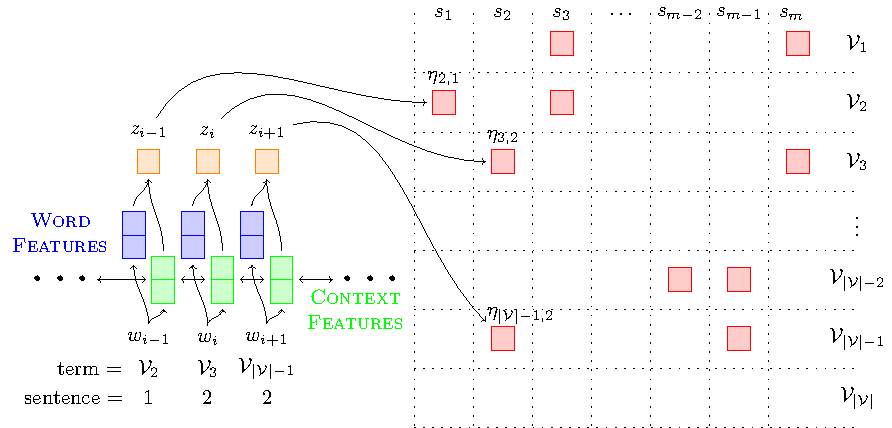
\includegraphics[scale=1.0]{dl_based_salience_models/figures/4_2_wimp_model.pdf}
 \end{center}
 \caption{(Left) Word and context features are extracted from the flat token
sequence representation to get word level importance scores 
$\wordImportance_i$. (Right) Word level scores are aggregated into a sparse
bag-of-words matrix with rows and columns corresponding to sentences and 
words respectively.}
\end{figure}

Our previous experiments revealed that lexical sematics were not the 
main driver of learning in sentence extractive news summarization. 
One could plausibly argue that it is a feature, not a bug, and that 
the structural
signals in news are intentional and not to be avoided. However, we think more 
attention could be paid to estimating importance scores at the word level.
We are motivated by potential application to abstractive generation: better
word level importance estimation could help to remove all but the most 
necessary content from the documents as a preprocessing stage before
abstractive summarization. We are also encouraged by practices
in multi-document news summarization, where word importance weights 
are the main ingredient in sentence representations. 


\newcommand{\classy}{\textsc{Classy}}
\newcommand{\occams}{\textsc{Occams}}

%\subsubsection{A brief discussion of \mlingsys.}

\occams{} and its antecedent \classy{} have been consistent top performers in various
summarization workshops \citep{conroyback,conroyclassy,davis2012occams}. 
In general their main approach 
is to represent each sentence as a sparse bag-of-words, where non-zero
entries correspond to word importance weights for the words found in the 
sentence. Typically, tf-idf weights are used for the importance scores.
The term by sentence matrix representing the document or documents to be
summarized is then factorized into two  matrices (typically with
non-negative entries) representing term factors and sentence factors.
The entries in the sentence factor matrix represent latent ``topics,'' 
and apriori the importance of each sentence is the sum of its latent topic
entries.

Sentence selection can subsequently be performed using one of several methods.
In the naive case, one can select the sentence with the highest vector norm, 
substract the selected latent factors from the remaining sentence vectors
(zeroing out any terms that become negative), and repeating until the
summary length budget is reached. More sophisticated selection procedures
involving multi-dimensional knapsack packing or submodular optimization 
can be used, however these are not the focus of this work.

One draw back to this approach is that the sentence factors and word 
importance scores are unsupervised with respect to the final summarization
objective; their utility to the summarization task is a happy coincidence.
Additionally, the word importance scores are not assigned based on the 
context in which the word appears.

We propose to address these issues by learning word level importance 
scores in the process of single document sentence extractive summarization.
Additionally, we propose a method of adapting these scores from the 
single document case to multi-document summarization.

\subsubsection{Proposed Model}


%In our proposed model for word importance, we first run the \elmo{}model 
%\citep{peters2018deep}
%over the input document to obtain contextual representations
%of each word. The \elmo{}embeddings are then combined with pretrained
%\glove embeddings along with embeddings for document frequency, 
%topic signature,
%sentence position, and part-of-speech tag, and then
%fed into a multi-layer perceptron to predict a scalar importance score.
%When a word occurs multiple times in the input, it can be given a different 
%importance score at each location because the \elmo{} embeddings will capture
%contributions of the salient neighbor words. A term-sentence matrix is 
%then formed from the input, using the estimated word importance scores 
%as the term weights. A sentence extractive summary can be obtained 
%using the naive sentence selection method described above or in 
%\autoref{alg:wimp_ext_alg}.
%The total score for the summary can also be obtained.
%
%We can train this summarizer using a gold extract sequence and a margin loss
%\[\objective(\theta) = \max\big(0, 1 + f(\predSaliences; \theta) - f(\saliences; \theta) \big) \] where $f(\predSaliences;\theta)$ is
%the score of our predicted extract summary.
%
%
%Let $\bowvec_1, \bowvec_2, \dots, \bowvec_n$ be the bag of words 
%representations of the 
%sentences selected for the summary, in the order they were selected.
%The score for the summary is computed as computed by the simple selection
%procedure would be
%$f() = \sum_{i=1}^n \sum_{j=1}^k \max(0, z_{i,j} - \sum_{l=1}^{i-1} z_{l,j})$ 
%
%
%~\\
%~\\

Let $\vocab$ be a finite vocabulary of words. A document $\doc$
is a sequence of $m$ words $(\word_1, \word_2, \ldots, \word_m) \in \vocab^m$.
We define two mappings of words to dense vector representations.
The first $\fdef{\wordFeatures}{\vocab}{\Rn{n_f}}$ maps words to 
a concatenation of feature embeddings whose total dimension is of size $n_f$. 
The various components of the feature embeddings include the word's \glove{} 
embedding, as well as embeddings for sentence position, document frequency,
and other word features that have been shown to be useful for summarization.
The second mapping
$\fdef{\contextFeatures}{\vocab}{\Rn{n_c}}$ maps the word to it's contextual
embedding; here this corresponds to the output of \elmo{} 
\citep{peters2018deep} at that word's
position in the document. 
The importance score $\wordImportance_i$ of a word $\word_i$ is the output of 
a feedforward layer 
\[ \wordImportance_i = \sigma\Big(\mathbf{v}^T \left[\begin{array}{c} \wordFeatures(\word_i) \\ \contextFeatures(\word_i) \end{array} \right] + b \Big) \]
    where $\mathbf{v} \in \Rn{n_f + n_c}$ and $b \in \R$ are learned weight
and bias parameters, and $\sigma$ is the logistic sigmoid.

Next, we aggregate the flat token level scores $\wordImportance_i$ into a
bag-of-words (BOW) 
representation for each sentence in the document.
Let $I_i$ be the set of indices of the flat word sequence corresponding
to the words in $i$-th input sentence. Then, let $\bow_i$ be the BOW 
representation of the $i$-th sentence with entries 
\[ \bow_{i,j} = \begin{cases} 
    0 & \textrm{if $\word_k \ne \vocab_j $ for all $k \in I_i $} \\ 
\sum_{k \in I_i} \mathbbm{1}\{\word_k = \vocab_j \} \cdot \wordImportance_k  & \textrm{otherwise}     \end{cases} \]
        for all $j \in \{1, \ldots, |\vocab|\}$.



\begin{figure}
  \begin{algorithmic}[1]
      \Procedure{\textsc{BowExtracter}}{$\bow_{1:n}, \beta, \kappa$}
   
      \State $\bow_i^{(1)}  \gets \bow_i \quad \forall i \in \{1, \ldots, n\}$
      \State $\hat{\eta} \gets 0$
      \State $t \gets 0$
      \While{ $\sum_{i=1}^t \kappa_{\predLabels_i} < \beta$ and $t < n$}
        \State $t \gets t + 1$
        \State $\predLabels_t \gets \operatorname{arg max}_{i \in \{1,\ldots, n\}}
            \sum_{j=1}^{|\vocab|} \bow^{(t)}_{i,j}$
            \State $\bow_i^{(t+1)} \gets \max(0, \bow_i^{(t)} - \bow^{(t)}_{\predLabels_t} )\quad  \forall i \in \{1, \ldots, n \}$
        \State $\hat{\eta} \gets \hat{\eta} + \sum_{j=1}^{|\vocab|} \bow_{\predLabels_t,j}^{(t)}$
         

      \EndWhile
        \State \Return $[\predLabels_1,\ldots,\predLabels_t], \hat{\eta}$ \Comment{Returns summary sentence indices and summary score.}
    \EndProcedure
  \end{algorithmic}
\caption{Simple sentence extraction algorithm given
 the sentence BOW representations $\omega_i$, 
  a word budget $\beta$, and a vector $\kappa$ of sentence lengths (in words)
  as input.}
\label{alg:wimp_ext_alg}
\end{figure}



        With the BOW representations in hand, we perform sentence selection
        using the algorithm presented in \autoref{alg:wimp_ext_alg} to 
        obtain a predicted extract indices $\predLabels$ and their associated
        overall summary score $\hat{\eta}$.

        We can optimize this model using a margin loss, where given a 
        gold extract sequence  $\labels$, we can compute the associated
        gold extract summary score $\eta$ and then minimize the following
        loss function \[\mathcal{L}_{ext}(\predLabels, \labels;\theta) = \max\big(0, 1 + \hat{\eta} - \eta\big)\]
        with respect to the parameters $\theta$ of the word importance 
        predictor.
        If needed, we can also introduce a supervised learning signal to the 
        individual word importance scores by collecting labels $\zeta_i$ for
        each $\wordImportance_i$ such that $\zeta_i = 1$ if $\word_i$ occurs
        and any human reference abstract and $0$ otherwise. The 
        $\objective_{ext}$ would then be augmented with an additional cross
        entropy loss for the word level predictions:
        \[ \mathcal{L}_{word}(\wordImportance, \zeta; \theta) = -\sum_{i=1}^m \zeta_i \log \wordImportance_i + (1 - \zeta_i) \log (1 - \wordImportance_i). \] 




        \paragraph{Adaptation to MDS} We also propose a simple 
        self attention-based modification to
        the word importance aggregation step to help adapt this method
        to multi-document summarization (MDS). \cite{conroy2013multilingual} 
        found
        that dimensionality reduction on the BOW representations improves
        summarizer performance in the MDS setting (but not as much on
 single document
        summarization). 


        We plan to experiment with the following importance 
        aggregation method. First, given the outputs of the contextual features
        $\mathbf{h}_i = \contextFeatures(\word_i)$, 
        we compute a self attention matrix $\Lambda \in \Rn{m\times m}$
        where \[\Lambda_{i,j} = \sigma(\mathbf{h}_i^T \mathbf{h}_j / \tau + b)  \]
        using sigmoidal attention \citep{kim2017structured} with a learned bias 
        parameter $b$ and a temperature parameter $\tau$.
        Next we compute an attention weighted word importance score $\bar{\wordImportance}_i$ for each word in the input using the following formula,
        \[ \bar{\wordImportance}_i = \sum_{j=1}^m \wordImportance_j \cdot \Lambda_{i,j}.\]
        We then use the aggregated word importance scores 
    $\bar{\wordImportance}_i$ inplace of their nonaggregated counterparts
        in the creating the BOW representations $\omega_j$.

        Our motivation is that by accumulating scores based on context
        similarity, words and topics that appear in multiple documents 
        will accumulate the bulk of the word importance scores, giving 
        an added boost to sentences that contain them. Implicitly, errant
        words from one document that are not on topic to the cluster will
        effectively not contribute much to a sentences score, reducing the 
        effectve dimension of the BOW vectors and regularizing individual
        sentences to the document cluster's mean.

        
        Since we are training our models on single documents, we expect that
        running our pretrainined word scoring model on the individual 
        documents from an MDS document cluster will result in 
        minimal task-adaptation mismatch. The remaining bias and temperature
        parameters can easily be tuned on the small amount of MDS training 
        data available.

%        We also plan to compare this method to using a non-negative matrix 
%        factorization 
%        method on the output of the learned BOW representation, 
%        and to hard attention assignments using Brown clustering.







%\subsubsection{
%\cite{conroy} 


 



\section{Deep Learning Models of Content Salience}
\label{sec:chapter4}
\label{sec:deep_learning_salience}


Increasingly, deep neural 
network models are being used to perform sentence extractive summarization 
tasks. While these models are very flexible and allow for easy hierarchical 
representation learning, it is unclear what signals they are extracting
from the data to make predictions.
In this section, we describe our completed experiments teasing out the 
importance
of different neural network designs for sentence level salience estimation
\citep{kedzie2018deep}. 
In particular, we experiment with several methods for encoding a sequence
of word embeddings into a sentence embedding, and then in turn, mapping
a sequence of sentence embeddings to sentence salience predictions. We 
introduce several simplifications to existing models in the literature, and
show their effectiveness on an SDS task across news, personal narratives,
workplace meetings, and medical journal article genres.

We also perform several diagnostic experiments 
and find impediments to learning robust models of 
sentence salience. In particular, the sentence position implicitly 
encoded in the models dominates the learning signal. While sentence position
is certainly an important feature in news, not all domains or tasks 
will share this feature;
 we would also like to be able to design
models that make their salience decisions primarily on lexical or
topical content.

We believe that the sentence embedding representation is too coarse to
make significant use of lexical information in the presence of less noisy
position features, even when position is only implicitly represented by 
the model.
To that end, we propose a new deep learning based SDS model that directly 
estimates individual word level salience scores, and a simple sentence 
selection and margin loss framework for learning. In this model,
we augment the word embeddings (which only capture shallow lexical semantics)
with embeddings representing other word features. Our initial experiments
suggest that document frequency, and information theoretic accounts of 
surprisal (e.g. topic signatures) are also useful for the summarization task. 
We expect to show less dependence on the position features using
the same ablation diagnostics we applied to our sentence level salience 
models. 
While previous work has estimated word importance using these features
in a linear model 
\citep{hong2014improving}, they were only able to take limited advantage of 
context features, i.e. taking a weighted average of word features to
the left and right. By contrast,
 in our proposed model we can combine rich
document specific contextual features, e.g. \textsc{Elmo} embeddings 
\citep{peters2018deep}, in conjunction with these word features.

Additionally, we plan to adapt this word level salience model to a news MDS task;
if it is less dependent on sentence position, it should be more amenable 
to MDS where lexical centrality to the document cluster is possibly
the dominant learning signal.  
%We concluded this section with proposed domain adaptation experiments for
%modifying the word importance model to work on a news MDS task. 
The MDS version of the model will use an importance score aggregation step
where word level scores accrue additional importance across documents 
using an attention mechanism.


In the next subsections we first briefly cover related work on sentence
and word level salience estimation before covering the 
completed sentence level
and proposed word level salience estimation experiments.
%are the
%This
%work describes impedements to learning and word and sentence representations
%in deep learning models of extractive summarization, and led to 
%a recent publication \citep{kedzie2018deep}. Based on these limitations,
%we propose extensions to the word level representations and explicitly model
%word level salience scores as a means to performing sentence extractive
%summarization. While the finished and proposed work focuses on single document
%summarization, we also propose an extension of the word level salience
%estimation model that we hope will generalize to the multi-document
%summarization context.















\subsection{Related Work}

Estimating sentence salience for summarization has often been approached as a 
sentence
classification problem. Na{\"i}ve Bayes 
\citep{kupiec1995trainable,teufel1997sentence,osborne2002using}, 
maximum entropy 
\citep{osborne2002using}, and support vector machine \citep{hirao2002ntt}
classifiers have all been applied to predict whether a sentence should
be included in an extract summary.
Sentence position features were a strongly predictive signal in all of these 
works.
Lexical features were more varied in their use; e.g., 
\cite{kupiec1995trainable} 
checked for the presence of key phrases from a manually curated list,
 \cite{osborne2002using} experimented with automatically extracted
bigram features, 
%of which only a small portion are actually discriminative,
while \cite{hirao2002ntt} used average \tfidf{} weights to capture
important lexical content.

While the previous works all estimated sentence salience independently,
a variety of structured prediction methods have also been explored
to jointly estimate the salience of sentences in a document or 
document cluster.
These include
hidden Markov models (HMMs) \citep{conroy2001text}, conditional random fields
(CRFs)
\citep{shen2007document}, large margin classifiers \citep{martins2009summarization}, and 
structured support vector
machines 
\citep{berg2011jointly,sipos2012large,durrett2016learning}. 
While positional or discourse features are important to all of these methods, 
\cite{martins2009summarization}, \cite{berg2011jointly}, and \cite{durrett2016learning} 
also learn lexical feature weights as part of their larger model.
Graph random walk based ranking has been another
prominent method for estimating salience of a collection of sentences 
jointly 
\citep{erkan2004lexrank,mihalcea2004textrank};
typically the sentence graphs are constructed using the cosine similarity
between a sentence's \tfidf{} weighted bag-of-words although other methods
of weighting graph edges have been used. Additionally, independent
sentence level priors about salience can also be incorporated by adjusting the 
probability of restarting the random walk \citep{erkan1001using,liu2008personalized}.


Deep learning methods have become the \textit{de facto} standard approach to many 
NLP problems, especially when there exists plentiful labeled data.
There has been a flurry of recent work on sentence extractive 
single document summarization of news using a variety of neural network 
architectures 
\citep{cheng2016neural,nallapati2016classify,nallapati2016summarunner,narayan2018ranking}.
These models have hierarchical representations of the document, using
either
recurrent neural networks (RNNs) or convolutional neural networks (CNNs)
to encode word embeddings into sentence embeddings which are then fed into
an RNN based sentence extractor. 
Unlike prior structured approaches,
finding the optimal label sequence in these models is intractable. However,
the richer word and sentence representations often yield better performance
even with a simpler inference method. 



%thanks in part to the availibilty of a large corpus 
%(approximately 300k) of CNN and Daily Mail articles with human written bullet 
%point summaries \citep{hermann2015teaching}.
%These models have typically built hierarchical representations of the text


%Comparing models and defining best practices for model design has become 
%difficult as papers often propose complex models with a variety
%of design choices, making it difficult to determine what choices actually
%lead to the best performance. 



There is also prior  work on estimating word importance directly 
(as opposed to learning word weights as a means to estimate sentence salience).
%Much of the summarization literature does not learn word importance weights, 
%but rather uses frequency derived proxies of importance instead 
%\citep{conroy2001text,shen2007document,sipos2012large,nenkova2005impact}.
%Other research has focused specifically on learning word importance weights
%directly. 
For example, \cite{yih2007multi} learn to predict the likelihood
of a term appearing in a summary using a maximum entropy classifier with
several document frequency and position features. \cite{hong2014improving}
extend these features to consider word type (e.g. named-entity type),
background information like the probability of the word occurring 
in a large collection of New York Times abstracts, and whether or
not the word occurs in an automatic summary (using an unsupervised summary
method). There does not appear to be much literature on extending this work
with deep learning, a gap we hope to fill with our proposed word level model. 
Outside of summarization,
\cite{sheikh2016learning} found that learning importance scores for 
words in a weighted bag-of-words model outperformed \tfidf{} based approaches
to text classification tasks like 
sentiment and topic detection. 
 


 



\subsection{Deep Learning Models of Sentence Salience}

 Given the diversity of neural architectural choices, a best practices
for sentence extracive summarization has yet to emerge. In this section
we ask what architecture design choices matter for single document 
summarization across a variety of domains.

We begin by definining some terminology. A sentence is represented as an
sequence of words $\sent = \word_1, \word_2, \ldots, \word_{|\sent|},$
where each word is drawn from a finite vocabulary $\vocab$ and $|\sent|$ is
the length of sentence $\sent$ in words. Similarly, a document $\doc =  
\sent_1, \sent_2, \ldots, \sent_{|\doc|} $ is a sequence of sentences, where 
$|\doc|$ is the size of the document in sentences.  

We treat sentence extractive summarization as a sequence tagging
problem: given a document $\doc$, we want to assign an associated binary
tag sequence $\Labels \in \{0,1\}^{\Sze{\doc}}$ such that the corresponding
set of extracts $\extracts = \{\sent_i \in \doc \; | \; \Labels_i =1 \}$ is
a suitable summary
of the document. Typically, it is assumed that the size of the extract summary
in sentences is much smaller than the input document, i.e. 
$|\extracts|  \ll |\doc|$.
It is also common to enforce a word budget $\budget$ such that
$\sum_{\sent \in \extracts} |\sent| \le \budget$.

A typical deep learning model will build up a hierarchical representation
of each sentence, starting at the word level, and then composing an arbitrarily
long sequence of word representations into a fixed length sentence 
representation.
First the individual words are 
projected to fixed length vectors, or word embeddings, via a mapping
$\embproj : \vocab
\rightarrow \mathbb{R}^{\embsize}$. The sentence encoder network $\encoder :
\{\mathbb{R}^{\embsize}\}^* \rightarrow \mathbb{R}^{\sembsize}$ is then 
responsible for mapping word embedding sequences to fixed length sentence 
embeddings. Finally, the sentence extractor network $\extractor : 
\{\mathbb{R}^\sembsize\}^* \rightarrow \{0, 1\}^*$ produces a label 
sequence $\Labels$.

We explore several choices of encoder and extractor architecture from the 
literature \citep{cheng2016neural,nallapati2016summarunner} as well as 
propose our own designs \citep{kedzie2018deep}. In the next sections,
we describe the different encoder and extractor architectures, before 
discussing data, experiments, and evaluation.

%the three sentence encoder architectures (\enAvg, 
%\enRnn, and \enCnn) followed by four extractor architectures 
%(\textit{rnn}, \textit{seq2seq}, \textit{sr}, and \textit{cl}).

\subsubsection{Sentence Encoders}
\paragraph{Averaging} This encoder simply averages a sentence's
associated word embeddings:
\[ \encoder_{avg}(\sent) = \frac{1}{|\sent|} \sum_{\word \in \sent} \embproj(\word). \]
Other than the word embeddings, this encoder involves no learned parameters,
and while it collapses word order, embedding averaging has consistently
been found competitive with more sophisticated sentence embedding techniques
\citep{iyyer2015deep,wieting2015towards,arora2016simple,wieting2017revisiting}.


\paragraph{Recurrent Neural Networks} The second encoder architecture
we experiment with is a recurrent neural network (RNN) over the word
embeddings. An RNN maintains an internal ``hidden'' state that is sequentially
updated upon observing each word embedding. In practice, we use a bidirectional
RNN with a gated recurrent unit (GRU) as the particular instantiation of 
the RNN cell \citep{cho2014learning}.
Under the RNN encoder, a sentence embedding for a sentence $\sent$ is defined 
as the concatenation of the final forward and backward GRU outputs,
\begin{align}
\encoder_{rnn}(\sent) = \Big[\overrightarrow{\semb}_{|\sent|}, \overleftarrow{\semb}_{1} \Big] & \\
  \rsemb_0 = \mathbf{0};& \quad 
  \rsemb_i = \rgru\left(\embproj(\word_i), \rsemb_{i-1}\right) \\
  \lsemb_{|\sent| + 1} = \mathbf{0};& \quad 
  \lsemb_i = \lgru\left(\embproj(\word_i), \lsemb_{i+1}\right) 
\end{align}
where $[\cdot]$ is the concatenation operator; $\rsemb_i$ and $\lsemb_i$ are
hidden states of the forward and backward GRU cells respectively; and 
$\rgru, \lgru : \mathbb{R}^\embsize \times \mathbb{R}^\sembsize 
\rightarrow \mathbb{R}^\sembsize$ are the forward and backward GRU cell 
operations.
\cite{nallapati2016summarunner} use a bidirectional RNN for their sentence
encoder.

\paragraph{Convolutional Neural Networks}
Our final sentence encoder uses a convolutional neural network
(CNN) to encode salient n-gram windows into a fixed length vector. 
CNN's have grown increasingly popular in many NLP tasks 
as a computationally efficient substitute for RNN-based architectures
\citep{kim2014convolutional,lei2015molding,dauphin2017language}.
Our architecture largely follows \cite{kim2014convolutional}: we apply a 
series of one dimensional convoluions over a sentence's word embeddings
using varying width convolutions. For each convolutional window size 
$\winsize \in \winsizes \subset \mathbb{N}$, a convolutional filter creates 
a feature vector $\cfeat{}{\winsize} \in \mathbb{R}^{\fmapsize_\winsize}$ 
and the encoder output is the concatenation of the $|\winsizes|$ vectors. 
The set of filter window sizes $\winsizes$ and the number of feature maps
$\fmapsize_\winsize$ for each $\winsize \in \winsizes$ are 
model hyperparameters.
Formally, we define the CNN encoding of a sentence $\sent$ as 
\begin{align}
\encoder_{cnn}(\sent) & = \left[\cfeat{}{\winsize} : \winsize \in \winsizes \right]\\
\cfeat{\cfidx}{\winsize} &= 
     \max_{i \in 1,\dots, |\sent| - \winsize + 1} 
       \relu\left(\cact_i \right) \\
\cact_i &= \cnnbias_\cfidx
    + \sum^{\winsize}_{j=1} \cnnweight_{\cfidx,j} \cdot \embproj(\word_{i + j -1})
\end{align}
where $\cnnbias \in \cnnBiasSpace$ and $\cnnweight \in \cnnWeightSpace$
are learned convolutional filter weights and $\relu(x) = \max(0, x)$ 
is the rectified linear unit \citep{nair2010rectified}. \cite{cheng2016neural}
use a CNN for their sentence encoder.

\subsubsection{Sentence Extractors}

A sentence extractor takes the encoder output, i.e. 
a sequence of sentence embeddings
$\encoder(\doc) =$ $\encoder(\sent_1), \ldots, \encoder(\sent_{|\doc|}) =
\semb_1, \ldots, \semb_{|\doc|}$, and produces an extract label sequence
$\Labels$. 
The sentence extractor is essentially a discriminative
classifier $p(\Labels_{1:\Sze{\doc}} | \semb_{1:\Sze{\doc}})$.
Previous neural network approaches to sentence extraction have assumed
an auto-regressive model, leading to a semi-Markovian
factorization of the extractor probabilities
$p(\Labels_{1:\Sze{\doc}} | \semb_{1:\Sze{\doc}})=\prod_{i=1}^{|\doc|} 
p(\Labels_i|\Labels_{<i},\semb_{1:\Sze{\doc}})$,
where each prediction $\Labels_i$ is dependent on \emph{all}
previous $\Labels_j$ for
all $j < i$. We compare two such models proposed by \cite{cheng2016neural}
and \cite{nallapati2016summarunner}.
A simpler approach that does not allow interaction among the $\Labels_{1:n}$
is to
model $p(\Labels_{1:\Sze{\doc}}|\semb_{1:\Sze{\doc}}) = 
\prod_{i=1}^{\Sze{\doc}} p(\Labels_i|\semb_{1:\Sze{\doc}})$,
  which we explore in two proposed extractor models that we refer to as the RNN 
  and Seq2Seq extractors.

\paragraph{SummaRunner Extractor}\citet{nallapati2016summarunner} proposed
a sentence extractor, which we refer to as the SummaRunner Extractor,
that factorizes the extraction probability into contributions 
from different sources.
First, a bidirectional RNN is run over the sentence embeddings\footnote{\citet{nallapati2016summarunner}
    use an RNN sentence encoder with 
this extractor architecture; in this work we pair the SummaRunner extractor
with different encoders. } and the output is
concatenated. A representation of the whole document is made by 
averaging the RNN output. A summary representation is also constructed 
by taking the sum of the previous RNN outputs weighted by their extraction
probabilities. Extraction predictions are made using 
the RNN output at the $i$-th prediction step, the document representation, and 
$i$-th version of the summary representation, along with factors for 
sentence location in the document. The use of the iteratively constructed
summary representation creates a dependence of $\Labels_i$ on all 
$\Labels_{<i}$.


In more detail, first the bidirectional RNN is applied to the input 
sentence embeddings,
\begin{align}
    \rExtHid_0 = \textbf{0}&\quad \quad \rExtHid_i = \rgru(\semb_i, \rExtHid_{i-1}) \\
    \lExtHid_{\Sze{\doc} + 1} = \textbf{0}& \quad \quad \lExtHid_i = \lgru(\semb_i, \lExtHid_{i+1}).
\end{align}

Then a document embedding $\demb$ is created by averaging in the hidden
RNN states and passing them through a feedforward layer: 
\begin{align}
    \demb = \tanh\left(\mathbf{b}_\doc + \mathbf{W}_\doc\frac{1}{\Sze{\doc}}
    \sum_{i=1}^{\Sze{\doc}} \left[\rExtHid_i; \lExtHid_i\right] \right).
\end{align}

The RNN outputs are then passed through a separate fully connected layer to 
create a sentece representation $\extHid_i$ where 
\begin{align}
    \extHid_i &= \relu\left(\mathbf{b}_z + \mathbf{W}_z \left[ \rExtHid,\lExtHid\right]\right)
\end{align}

The extraction probability is then determined by contributions from five 
sources:
\begin{align}
    \textit{sentence salience} &\quad a^{(sent)}_i=\mathbf{W}^{(sent)} \extHid_i, \\
    \textit{document salience}&\quad a^{(doc)}_i = \extHid_i^T\mathbf{W}^{(doc)} \demb, \\
    \textit{summary novelty}&\quad a^{(nov)}_i = -\extHid_i^T\mathbf{W}^{(nov)} \smemb_i, \label{eq:srnov} \\
    \textit{fine-grained position}&\quad a^{(fpos)}_i = \mathbf{W}^{(fpos)} 
    \posemb_i, \\
    \textit{coarse-grained position}&\quad a^{(cpos)}_i = \mathbf{W}^{(cpos)} 
    \qrtemb_i,
\end{align}
where $\posemb_i$ and $\qrtemb_i$ are embeddings associated with the $i$-th sentence
position and the quarter of the document containing sentence $i$ respectively.
In \autoref{eq:srnov}, $\smemb_i$ is a representation of the summary after
making the first $i-1$ predictions, and is 
computed as the
sum of the previous $\extHid_{<i}$ weighted by their extraction probabilities,
\begin{align}
    \smemb_i & = \tanh\left(\sum_{j=1}^{i-1} p(\Labels_j=1|\Labels_{<j},\semb_{1:\Sze{\doc}}) \cdot \extHid_j\right), \quad\quad \smemb_1 = \mathbf{0}.
\end{align}
Note that the presence of this term induces dependence of each 
$\Labels_i$ to 
all $\Labels_{<i}$. % similarly to the Cheng \& Lapata extractor.
The final extraction probability is the logistic sigmoid of the
sum of these terms plus a bias,
\begin{align}
    p(\Labels_i=1|\Labels_{<i}, \semb_{1:\Sze{\doc}}) &= \sigma\left(
      a_i^{(sent)} + a_i^{(doc)} + a_i^{(nov)} 
  + a_i^{(fpos)}  + a_i^{(cpos)} + b \right).
    %p(\Labels_i=1|\Labels_{<i}, \semb_{1:\Sze{\doc}}) &= \sigma\left(\begin{array}{l}
 %     a_i^{(con)} + a_i^{(sal)} + a_i^{(nov)} \\
 % + a_i^{(pos)}  + a_i^{(qrt)} + b \end{array}\right).
\end{align}
The weight matrices $\mathbf{W}_\doc$, $\mathbf{W}_z$, $\mathbf{W}^{(sent)}$,
$\mathbf{W}^{(sal)}$, $\mathbf{W}^{(nov)}$, $\mathbf{W}^{(fpos)}$,
$\mathbf{W}^{(cpos)}$ and bias terms $\mathbf{b}_\doc$, $\mathbf{b}_z$, and 
$b$ 
are learned parameters;
additionally, the GRUs have separate learned parameters.
%

\paragraph{RNN Extractor \citep{kedzie2018deep}}
    Our first proposed model is a very simple bidirectional
RNN based tagging model, and can be thought of as a 
bare bones version of the SummaRunner
extractor. In this model, we pass the outputs of a bidirectional GRU over the 
sentence embeddings into a multi-layer perceptron that terminates in a layer 
of
sigmoid activations corresponding to the sentence level extraction probabilities.
%sentence encoder we use a GRU cell.
%The forward and backward outputs of each sentence are passed through a 
%multi-layer perceptron with a logsitic sigmoid output 
%to predict the probability
%of extracting each sentence. 
%See \autoref{fig:extractors}.a for a graphical layout.
%and \autoref{app:rnnextractor} for details.


%\newcommand{\rExtHidden}{\overrightarrow{h}}
%\newcommand{\lExtHidden}{\overrightarrow{h}}
%\newcommand{\docSize}{|\doc|}
%\newcommand{\logits}{o}

\begin{align}
    \rExtHid_0 = \mathbf{0} &\quad\quad   \rExtHid_i = \rgru(\semb_i, \rExtHid_{i-1}) \\
    \lExtHid_{\Sze{\doc} + 1} = \mathbf{0}&\quad \quad    \lExtHid_i = \lgru(\semb_i, \lExtHid_{i+1}) \\
    \mathbf{o}_i &= \relu\left(\mathbf{U} \cdot [\rExtHid_i; \lExtHid_i] + \mathbf{u} \right)\\
    p(\Labels_i=1|\semb_{1:\Sze{\doc}}) &= \sigma\left(\mathbf{v}\cdot \mathbf{o}_i + v  \right)
\end{align}
where $\rgru$ and $\lgru$ indicate the 
forward and backward GRUs respectively, and each have separate learned 
parameters; $\mathbf{U}, \mathbf{v}$ and $u, v$ are learned weight and 
bias parameters respectively.


\paragraph{Cheng \& Lapata Extractor} 
 This extractor, proposed by 
\citet{cheng2016neural}, %, which we refer to as the Cheng \& Lapata Extractor,
is built around a sequence-to-sequence model.
First, each sentence embedding\footnote{\citet{cheng2016neural} used an CNN sentence encoder with 
this extractor architecture; in this work we pair the Cheng \& Lapata extractor
with several different encoders.} is
fed into an encoder side RNN, with the final encoder state passed to the
first step of the decoder RNN. On the decoder side, the same sentence 
embeddings are fed as input to the decoder and both encoder and decoder 
outputs are used to predict each $\Labels_i$. The decoder input is weighted by the previous 
extraction
probability, inducing the dependence of $\Labels_i$ on $\Labels_{<i}$.


The basic architecture is a
sequence-to-sequence
model defined as follows:
\begin{align}
    \enextHid_0 = \textbf{0}& \quad \quad   \enextHid_i = \gru_{enc}(\semb_i, \enextHid_{i-1}) \\
    \deextHid_1 = \gru_{dec}(\semb_*, \enextHid_{\Sze{\doc}}) &\quad\quad
\deextHid_i = \gru_{dec}(p_{i-1} \cdot \semb_{i-1}, \deextHid_{i-1}) \label{eq:cl1} \\
\mathbf{o}_i &= \relu\left(\mathbf{U} \cdot [\enextHid_i; \deextHid_i] + \mathbf{u} \right)\\
p_i = p(\Labels_i=1|\Labels_{<i}, \semb_{1:\Sze{\doc}}) &= \sigma\left(\mathbf{v}\cdot \mathbf{o}_i + v  \right) 
\end{align}
where $\semb_*$ is a learned ``begin decoding'' sentence embedding;
each GRU has separate learned 
parameters; and $\mathbf{U}, \mathbf{v}$ and $u, v$ are learned weight and bias parameters.
Note in \autoref{eq:cl1} that 
the decoder side GRU input is the sentence embedding from the previous time
step weighted by its probabilitiy of extraction ($p_{i-1}$) from the 
previous step, inducing dependence of each output $\Labels_i$ on all previous 
outputs $\Labels_{<i}$.



\paragraph{Seq2Seq Extractor \citep{kedzie2018deep}} 
%One shortcoming of the RNN extractor is that long range
%information from one end of the document may not easily be able to affect 
%extraction probabilities of sentences at the other end. 
Our second proposed model, the represents a more typical sequence-to-sequence
architecture with dot product style attention \citep{luong2015effective},
%mitigates this problem with an 
%attention 
%mechanism commonly
used for neural machine translation \cite{bahdanau2014neural} and 
abstractive summarization \cite{see2017get}. 
The sentence embeddings are first
encoded by a bidirectional $\gru$. A separate decoder $\gru$ transforms each 
sentence into a query vector which attends to the encoder output. The
attention weighted encoder output and the decoder $\gru$ output are concatenated
and fed into a multi-layer perceptron to compute the extraction probability.
%See \autoref{fig:extractors}.b for a graphical layout.
Unlike the Cheng \& Lapata extractor, the Seq2Seq extractor does not induce 
dependencies between the extraction labels, i.e. they are conditionally independent.

The architecture is defined as follows
\begin{align}
    \enextHid_0 = \textbf{0}& \quad \quad   \enextHid_i = \gru_{enc}(\semb_i, \enextHid_{i-1}) \\
    \deextHid_0 = \gru_{dec}(\semb_*, \enextHid_{\Sze{\doc}}) &\quad\quad
\deextHid_i = \gru_{dec}(\semb_{i}, \deextHid_{i-1}) \label{eq:cl1} \\
 \alpha_{i,j} = 
   \frac{\exp \left(\deextHid_i \cdot \enextHid_j \right)}{
   \sum_{j=1}^{\Sze{\doc}}\exp\left(\deextHid_i \cdot \enextHid_j\right)}
& \quad\quad \bar{\enextHid}_i = \sum_{j=1}^{\Sze{\doc}} \alpha_{i,j} \enextHid_j \\
\mathbf{o}_i &= \relu\left(\mathbf{U} \cdot [\bar{\enextHid}_i; \deextHid_i] + \mathbf{u} \right)\\
p(\Labels_i=1|\semb_{1:\Sze{\doc}}) &= \sigma\left(\mathbf{v}\cdot \mathbf{o}_i + v  \right) 
\end{align}
where $\semb_*$ is a learned ``begin decoding'' sentence embedding;
each GRU has separate learned 
parameters; and $\mathbf{U}, \mathbf{v}$ and $u, v$ are learned weight and 
bias parameters. In practice, we run this model in ``bidirectional mode'' 
where seperate sequence-to-sequence model also run in the reverse direction,
equations 28-29 are computed using the concatenation of the encoder/decoder
outputs. 

\subsubsection{Data}
\begin{table}
 \centering
    \begin{tabular}{ r  r r r r }
      \toprule
      \textbf{Dataset} & \textbf{Train} & \textbf{Valid} & \textbf{Test} &
        \textbf{Refs} \\
      \midrule
      CNN/DailyMail & 287,113 & 13,368 & 11,490 & 1\\
      NYT & 44,382 & 5,523 & 6,495 & 1.93\\
      DUC & 516 & 91 & 657 & 2 \\
      Reddit & 404 & 24 & 48 & 2 \\
      AMI & 98 & 19 & 20 & 1 \\
      PubMed & 21,250 & 1,250 & 2,500 & 1\\
      \bottomrule
    \end{tabular}
   \caption{Sizes of the training, validation, test splits for each dataset
   and the average number of test set human reference abstracts per document.}
   \label{tab:dldata}
\end{table}



We perform our experiments across six corpora from varying domains to 
understand how different biases within each domain can affect content 
selection. The corpora come from the news domain
(CNN-DailyMail, New York Times, DUC), personal narratives domain (Reddit),
workplace meetings (AMI), and medical journal articles (PubMed). See 
\autoref{tab:data} for dataset statistics.


\paragraph{CNN-DailyMail} We use the preprocessing and training, validation, 
and test splits
of \cite{see2017get}.
This corpus is a mix of news on different topics including politics,
sports, and entertainment.

\paragraph{New York Times}The New York Times (NYT) corpus \citep{sandhaus2008new} contains
 two types of abstracts for a subset of its articles. The first summary is
an archival abstract and the 
second is a shorter online teaser meant to entice a viewer of the webpage to
click to read more. From this collection, we take all articles that have 
a concatenated summary length of at least 100 words.
We create training, validation, and test splits by partitioning on dates;
we use the year 2005 as the validation data, with training and test partitions
including documents before and after 2005 respectively.

\paragraph{DUC} We use the single document summarization data from the 2001
and 2002
Document Understanding Conferences (DUC) \citep{over2002introduction}. We split the 2001 data into training
and validation splits and reserve the 2002 data for testing.

\paragraph{AMI} The AMI corpus \citep{carletta2005ami} 
is a collection of real and staged office meetings
annotated with text transcriptions, along with abstractive
summaries. We use the prescribed splits. 

\paragraph{Reddit} \citet{ouyang2017crowd} collected a corpus of personal 
    stories shared
 on Reddit\footnote{\url{www.reddit.com}} along with multiple extractive 
 and abstractive summaries. We randomly split this data using roughly three and five percent of the data validation and test respectively.

\paragraph{PubMed}{We created a corpus of 25,000 randomly sampled
    medical journal articles from the PubMed Open Access 
    Subset\footnote{\url{https://www.ncbi.nlm.nih.gov/pmc/tools/openftlist/}}.
    We only included articles if they were at least 1000 words long and 
    had an abstract of at least 50 words in length.
We used the article abstracts as the ground truth human summaries.}

\paragraph{Ground Truth Extract Summaries}
Since we do not typically have ground truth extract summaries from which to
create the labels $\Labels_i$, we construct gold label sequences 
by greedily optimizing \rougeN{1} as in \cite{nallapati2016summarunner}.
We choose to optimize for \rougeN{1} rather than 
\rougeN{2} similarly to other optimization based approaches to summarization 
\cite{sipos2012large,durrett2016learning,nallapati2016summarunner} 
which found this to be the easier target to learn.






\subsubsection{Experiments}

 We are interested in two questions. The first, more pragmatic question, is
 what are the best configuration of encoder/extractor architectures?
 We answer this question by evaluating \rouge{} recall and \meteor{} 
\citep{denkowski:lavie:meteor-wmt:2014}
 performance across our six collected datasets. We perform the standard
 stochastic gradient descent based optimization (using the Adam
 update \citep{kingma2014adam}) of the weighted negative log likehood 
 \[ \mathcal{L}(\theta) = -\sum_{\doc, \Labels \in \mathcal{D}} 
            \sum_i \omega(\Labels_i) 
        \log p(\Labels_i|\Labels_{<i}, \encoder(\doc); \theta) \]
        where $\theta$ are model parameters and $\omega(\Labels_i)$ upweights
        the positive labels to account for the imbalanced label distribution.

% We lack human reference extract labels for our datasets and so we obtain
% said lable sequences heuristically, by finding a label sequence $\Labels^*$
% by greedily optimizing ROUGE-1 recall with respect to the human reference
% abstracts.

 The second question, is more diagnostic in nature: what signals
 in the data are driving model learning?
 We perform several experiments to find answers. 
 We hypothesize that the lexical semantics encoded at the word embedding
 level will be important to subsequent sentence representations, and
 perform a comparison on learning with and with out fine tuning of the 
 embeddings. In both cases, embeddings are initialized with Glove
 embeddings pretrained on Wikipedia and Gigaword \citep{pennington2014glove}.
 
 
 We also hypothesize that certain classes of words will be more important 
 to identifying salient content than others. We perform word ablation 
 experiments where we alternately remove nouns, verbs, adjectives \& adverbs,
 and function words from the sentence encoder input and compare performance 
 to the non-ablated system. We expect that the nouns will be more important
 to content selection. 


 Our final experiments attempt to tease out the effect of structural features 
 from the lexical. In this experiment, we shuffle the sentence order at 
 training time. In this setup, we obfuscate features about which content 
 was introduced in the article first, an important and well known bias in 
 news domain \citep{nenkova2005automatic}. 

 

 \subsubsection{Results}

 %?\begin{table*}[ht]
%?    \center
%?    \begin{tabular}{ccggccggccggcc}
%?        \toprule
%?        \multirow{2}{*}{\textbf{Ext.}} &\multirow{2}{*}{\textbf{Enc.}}  & \multicolumn{2}{g}{\textbf{CNN/DM}} & \multicolumn{2}{c}{\textbf{NYT}} & \multicolumn{2}{g}{\textbf{DUC 2002}} & \multicolumn{2}{c}{\textbf{Reddit}} & \multicolumn{2}{g}{\textbf{AMI}} & \multicolumn{2}{c}{\textbf{PubMed}}\\
%?         &  & M & R-2 & M & R-2 & M & R-2 & M & R-2 & M & R-2 & M & R-2\\
%?        \midrule
%?%        Random &  -- & 18.2 & 12.7 & 20.7 & 16.0 & 21.7 & 15.8 & \textbf{20.4} & \textbf{12.9} & 12.7 &  2.0 & 16.9 &  9.3\\
%?%        \hline
%?        Lead &  -- & 24.1 & 24.4 & 30.0 & 32.3 & 25.1 & 21.5 & \textbf{20.1} & \textbf{10.9} & 12.3 &  2.0 & 15.9 &  9.3\\
%?%        \hline
%?%        Tail &  -- & 13.7 &  5.4 & 12.5 &  4.1 & 17.8 &  9.1 & \textbf{19.8} & \textbf{10.0} & 11.5 &  2.7 & 17.0 &  9.9\\
%?        \hline
%?        \multirow{3}{*}{RNN} & Avg. & \textbf{25.2} & 25.4 & 29.8 & 34.7 & \textbf{26.8} & 22.7 & \textbf{20.4} & \textbf{11.4} & \textbf{17.0} & \textbf{ 5.5} & 19.8 & 17.0\\
%?         & RNN & 25.1 & 25.4 & 29.6 & 34.9 & \textbf{26.8} & 22.6 & \textbf{20.2} & \textbf{11.4} & 16.2 & \textbf{ 5.2} & 19.7 & 16.6\\
%?         & CNN & 25.0 & 25.1 & 29.0 & 33.7 & \textbf{26.7} & \textbf{22.7} & \textbf{20.9} & \textbf{12.8} & 14.4 &  3.2 & 19.9 & 16.8\\
%?        \hline
%?        \multirow{3}{*}{Seq2Seq} & Avg. & \textbf{25.2} & \textbf{25.6} & \textbf{30.5} & \textbf{35.7} & \textbf{27.0} & \textbf{22.8} & \textbf{20.9} & \textbf{13.6} & \textbf{17.0} & \textbf{ 5.5} & \textbf{20.1} & \textbf{17.7}\\
%?         & RNN & \textbf{25.1} & 25.3 & 30.2 & \textbf{35.9} & \textbf{26.7} & 22.5 & \textbf{20.5} & \textbf{12.0} & 16.1 & \textbf{ 5.3} & 19.7 & 16.7\\
%?         & CNN & 25.0 & 25.1 & 29.9 & 35.1 & \textbf{26.7} & \textbf{22.7} & \textbf{20.7} & \textbf{13.2} & 14.2 &  2.9 & 19.8 & 16.9\\
%?        \hline
%?    \multirow{3}{*}{\begin{tabular}{c} Cheng \\ \& \\ Lapata \end{tabular}} & Avg. & 25.0 & 25.3 & 30.4 & \textbf{35.6} & \textbf{27.1} & \textbf{23.1} & \textbf{20.9} & \textbf{13.6} & \textbf{16.7} & \textbf{ 6.1} & \textbf{20.1} & \textbf{17.7}\\
%?         & RNN & 25.0 & 25.0 & \textbf{30.3} & \textbf{35.8} & \textbf{27.0} & \textbf{23.0} & \textbf{20.3} & \textbf{12.6} & \textbf{16.3} & \textbf{ 5.0} & 19.7 & 16.7\\
%?         & CNN & \textbf{25.2} & 25.1 & 29.9 & 35.0 & \textbf{26.9} & \textbf{23.0} & \textbf{20.5} & \textbf{13.4} & 14.3 &  2.8 & 19.9 & 16.9\\
%?        \hline
%?    \multirow{3}{*}{\begin{tabular}{c}Summa \\ Runner \end{tabular} } & Avg. & 25.1 & 25.4 & 30.2 & 35.4 & 26.7 & 22.3 & \textbf{21.0} & \textbf{13.4} & \textbf{17.0} & \textbf{ 5.6} & 19.9 & 17.2\\
%?         & RNN & 25.1 & 25.2 & 30.0 & 35.5 & 26.5 & 22.1 & \textbf{20.9} & \textbf{12.5} & \textbf{16.5} & \textbf{ 5.4} & 19.7 & 16.5\\
%?         & CNN & 24.9 & 25.0 & 29.3 & 34.4 & 26.4 & 22.2 & \textbf{20.4} & \textbf{12.3} & 14.5 &  3.2 & 19.8 & 16.8\\
%?        \hline
%?        Oracle & -- & 31.1 & 36.2 & 35.3 & 48.9 & 31.3 &  31.8 & 24.3 &  16.2 &8.1 &  3.9  & 24.1 &25.0 \\
%?        \bottomrule
%?    \end{tabular}
%?%?
%?%?    \caption{METEOR (M) and ROUGE-2 recall (R-2)  results across all 
%?%?        extractor/encoder pairs.
%?%?           Results that are statistically indistinguishable from the best 
%?%?           system are shown in bold face.}
%?%?  \label{tab:results}
%?\end{table*}


\begin{table*}[ht]
    \center
    \begin{tabular}{ccgcgcgc}
        \toprule
            \textbf{Extractor}   & \textbf{Encoder}
          & \textbf{CNN/DM} & \textbf{NYT} & \textbf{DUC} 
          & \textbf{Reddit} & \textbf{AMI} & \textbf{PubMed}\\
      %   &  & R-2 & R-2 & R-2 & M & R-2 & M & R-2 & M & R-2\\
        \midrule
%        Random &  -- & 18.2 & 12.7 & 20.7 & 16.0 & 21.7 & 15.8 & \textbf{20.4} & \textbf{12.9} & 12.7 &  2.0 & 16.9 &  9.3\\
%        \hline
        Lead &  -- & 24.4 & 32.3 & 21.5 & \textbf{10.9} &  2.0 &  9.3\\
%        \hline
%        Tail &  -- & 13.7 &  5.4 & 12.5 &  4.1 & 17.8 &  9.1 & \textbf{19.8} & \textbf{10.0} & 11.5 &  2.7 & 17.0 &  9.9\\
        \hline
        \multirow{3}{*}{RNN} 
 & Avg. & 25.4 & 34.7 & 22.7 & \textbf{11.4} & \textbf{5.5} & 17.0\\
 & RNN & 25.4 & 34.9 & 22.6 & \textbf{11.4} & \textbf{ 5.2} & 16.6\\
 & CNN & 25.1 & 33.7 & \textbf{22.7} & \textbf{12.8} &  3.2 & 16.8\\
        \hline
        \multirow{3}{*}{Seq2Seq} 
        & \textcolor{red}{Avg.} & \textbf{25.6} & \textbf{35.7} & \textbf{22.8} & \textbf{13.6} & \textbf{ 5.5} & \textbf{17.7}\\
 & RNN & 25.3 & \textbf{35.9} & 22.5 & \textbf{12.0} & \textbf{ 5.3} & 16.7\\
 & CNN & 25.1 & 35.1 & \textbf{22.7} & \textbf{13.2} &  2.9 & 16.9\\
        \hline
    \multirow{3}{*}{\begin{tabular}{c} Cheng \\ \& \\ Lapata \end{tabular}} 
& Avg. & 25.3 & \textbf{35.6} & \textbf{23.1} & \textbf{13.6} & \textbf{ 6.1} & \textbf{17.7}\\
& RNN & 25.0 & \textbf{35.8} & \textbf{23.0} & \textbf{12.6} & \textbf{ 5.0} & 16.7\\
         & CNN & 25.1 & 35.0 & \textbf{23.0} & \textbf{13.4} &  2.8 & 16.9\\
        \hline
    \multirow{3}{*}{\begin{tabular}{c}Summa \\ Runner \end{tabular} } 
         & Avg. & 25.4 & 35.4 & 22.3 & \textbf{13.4} & \textbf{ 5.6} & 17.2\\
         & RNN & 25.2 & 35.5 & 22.1 & \textbf{12.5} & \textbf{ 5.4} & 16.5\\
         & CNN & 25.0 & 34.4 & 22.2 & \textbf{12.3} &  3.2 & 16.8\\
        \hline
        Oracle & -- & 36.2 & 48.9 &  31.8 &  16.2 &  3.9  &25.0 \\
        \bottomrule
    \end{tabular}

    \caption{\textbf{Overall Results} \rougeN{2} recall  results across all 
        extractor/encoder pairs.
           Results that are statistically indistinguishable from the best 
           system are shown in bold face.}
  \label{tab:results}
\end{table*}

  

The results of our main experiment comparing 
the different extractors/encoders are shown in 
Table~\ref{tab:results}.
Overall, we find no major advantage when using the CNN and RNN sentence
encoders over the averaging encoder. The best performing encoder/extractor pair either 
uses the averaging 
encoder (five out of six datasets) or the differences 
are not statistically significant. %When only comparing within the 
%same extractor choice,  the averaging encoder is the better choice
%in 14 of 20 cases. 
%\hal{i wonder if it would be worth adding another ``average performance metric'' column to \autoref{tab:results}.
%  i'm thinking have ``Average $\Delta$-Best'' meaning how far (on average across the datasets) is this setting from the best setting available on that dataset.
%  so since the best numbers are: 25.56, 35.85, 23.11, 13.65, 5.63
%  and the first row numbers are: 25.42, 34.67, 22.65, 11.37, 5.50
%  then the deltas are:            0.14,  1.18,  0.46,  2.28, 0.13
%  the the average delta is 0.84 (assuming my math is right)
%  there's an argument to do multiplicative, in which case
%  the multipliers for first row:  0.99,  0.97,  0.98,  0.83, 0.97
%  and the average is 0.95
%  either way this gives a quick way to make comparisons between rows. you could do the same for the other tables too.}

  %\hal{in some of the tables you list R-2 as headers even though all the numbers are R-2. just put that in the caption.}


When looking at extractors, the Seq2Seq extractor is either part of 
the best performing system (three out of six datasets) or is not 
statistically distinguishable from the best extractor. 

Overall, on the news and medical journal domains, the differences are 
quite small with the 
differences between worst and best systems on the CNN/DM dataset 
spanning only .56 of a ROUGE point. While there is more performance variability
 in the Reddit and AMI data, there is less distinction among systems: 
 no differences are significant on Reddit
and every extractor has at least one configuration that is indistinguishable
from the best system on the AMI corpus. This is probably due to the small test
size of these datasets.
%\hal{this is probably at least partially because of test set size. maybe mention this.}





%?\textcolor{red}{Overall we find that the \modelTwoBF~extractor achieves the 
%?best ROUGE scores on three out of four domains (STILL RUNNING ON AMI AND PUBMED). 
%?However, most
%?differences are not signficant. (Need to discuss stat sig and how to show it).}
%?On the larger CNN-DailyMail dataset, especially, 
%?differences are quite smail across all extractor/encoder pairs.
%?The \baselineOneBF~extractor achieves the best performance on the DUC 2002
%?dataset. It is disappointing that the \baselineOneBF~and \baselineTwoBF~based 
%?models do not gain any apparent advantage in conditioning on previous 
%?sentence selection decisions; this result suggests the need to improve
%?the representation of the summary as it is being constructed iteratively.
%?
%?\textbf{Choice of Encoder} We also find there to be no major advantage 
%?between the different sentence encoders. \textcolor{red}{In most cases,
%?there is no statistical significance between the averaging encoder and either
%?the RNN or CNN encoders.} 

%The lack of differentiation amongst the different encoders concerning; one
%would assume learning with the appropriate structure would be helpful.
%The results of next 




 
\begin{table*}[t]
\center
\begin{tabular}{ccgL{.5cm}cm{.5cm}gL{.75cm}cm{.75cm}gL{.75cm}cm{.5cm}}
    \toprule
    \multirow{1}{*}{\textbf{Ext.}} &\multirow{1}{*}{\textbf{Emb.}}  & \multicolumn{2}{g}{\textbf{CNN/DM}} & \multicolumn{2}{c}{\textbf{NYT}} & \multicolumn{2}{g}{\textbf{DUC}} & \multicolumn{2}{c}{\textbf{Reddit}} & \multicolumn{2}{g}{\textbf{AMI}} & \multicolumn{2}{c}{\textbf{PubMed}}\\
   %  &  & R-2 & R-2 & R-2 & R-2 & R-2 & R-2\\
   % \hline
    \midrule
%    \multirow{2}{*}{RNN} & Fixed & \textbf{25.4} & & \textbf{34.7} & & \textbf{22.7} & & \textbf{11.4} & & \textbf{ 5.5} & & \textbf{17.0}\\
%                         & Learn & 25.2& \footnotesize{(0.2)} & 34.3 &\footnotesize{(0.4)} & \textbf{22.6} & \footnotesize{(0.1)} & \textbf{11.3} & \footnotesize{(0.1)} & \textbf{ 5.3} & \footnotesize{(0.2)} & 16.4& \footnotesize{(0.6)}\\
%    \hline
    \multirow{2}{*}{Seq2Seq} & Fixed & \textbf{25.6} && \textbf{35.7}& & \textbf{22.8}& & \textbf{13.6} &&  5.5 && \textbf{17.7}\\
   & Learn & 25.3 &\footnotesize{(0.3)} & \textbf{35.7}& \footnotesize{(0.0)} & \textbf{22.9} & \footnotesize{(-0.1)} & \textbf{13.8} &\footnotesize{ (-0.2)} & \textbf{ 5.8} & \footnotesize{(-0.3)} & 16.9 & \footnotesize{(0.8)}\\
%    \hline
%    \multirow{2}{*}{C\&L} & Fixed & \textbf{25.3} && \textbf{35.6} && \textbf{23.1} && \textbf{13.6} && \textbf{ 6.1} && \textbf{17.7}&\\
%                      & Learn & 24.9 &\footnotesize{(0.4)} & 35.4 & \footnotesize{(0.2)} & \textbf{23.0} &\footnotesize{ (0.1)} & \textbf{13.4} &\footnotesize{ (0.2)} & \textbf{ 6.2} &\footnotesize{ (-0.1)} & 16.4 &\footnotesize{ (1.3)} \\
%    \hline
%\multirow{2}{*}{\begin{tabular}{c} Summa \\ Runner \end{tabular}} & Fixed & \textbf{25.4} && \textbf{35.4} && \textbf{22.3} && \textbf{13.4} && \textbf{ 5.6} & &\textbf{17.2}&\\
%                                                                  & Learn & 25.1 &\footnotesize{(0.3)} & 35.2 &\footnotesize{(0.2)} & \textbf{22.2} & \footnotesize{(0.1)} & 12.6 & \footnotesize{(0.8)} & \textbf{ 5.8} & \footnotesize{(-0.2)} & 16.8&\footnotesize{ (0.4) }\\
    \bottomrule
\end{tabular}

\caption{ROUGE-2 recall across sentence extractors
    when using fixed pretrained embeddings or when embeddings are updated during training. In both cases embeddings
    are initialized with pretrained GloVe embeddings. All extractors use the averaging 
sentence encoder. When both learned and fixed settings are bolded,
there is no signifcant performance difference. RNN extractor is omitted for space but is similar to Seq2Seq. Difference in scores shown in parenthesis.}
\label{tab:embeddings}
\end{table*}

%\begin{table*}
%\center
%\begin{tabular}{| c | c || c | c | c | c | c | c | c | c |}
%\hline
%  &   & \multicolumn{2}{|c|}{cnn-dailymail} & \multicolumn{2}{|c|}{nyt} & \multicolumn{2}{|c|}{duc-sds} & \multicolumn{2}{|c|}{reddit} \\
%system & embeddings & R1 & R2  & R1 & R2  & R1 & R2  & R1 & R2  \\
%\hline
%\multirow{2}{*}{RNN} & fixed & 55.3 & 25.4 & 51.4 & 34.7 & 44.1 & 22.6 & 45.2 & 11.4\\ \cline{2-10}
% & learned & 55.1 & 25.2 & 51.1 & 34.3 & 44.1 & 22.6 & 45.3 & 11.3\\
%\hline
%\multirow{2}{*}{Seq2Seq} & fixed & 55.6 & 25.6 & 52.5 & 35.7 & 44.4 & 22.8 & 49.1 & 13.6\\ \cline{2-10}
% & learned & 55.2 & 25.3 & 52.4 & 35.7 & 44.5 & 22.9 & 49.4 & 13.8\\
%\hline
%\multirow{2}{*}{C\&L} & fixed & 55.1 & 25.3 & 52.3 & 35.6 & 44.8 & 23.1 & 48.3 & 13.6\\ \cline{2-10}
% & learned & 54.8 & 25.0 & 52.1 & 35.4 & 44.6 & 23.0 & 48.6 & 13.5\\
%\hline
%\multirow{2}{*}{SummaRunner} & fixed & 55.3 & 25.4 & 52.1 & 35.4 & 44.0 & 22.3 & 48.8 & 13.4\\ \cline{2-10}
% & learned & 55.0 & 25.1 & 52.0 & 35.2 & 43.8 & 22.1 & 47.8 & 12.6\\
%\hline
%\end{tabular}
%\caption{ROUGE 1 and 2 recall results across different sentence extractors
%    when using learned or pretrained embeddings. In both cases embeddings
%    are initialized with pretrained GloVe embeddings. All results are 
%averaged from five random initializations. All extractors use the averaging 
%sentence encoder.}
%\label{tab:embeddings}
%\end{table*}

\paragraph{Word Embedding Learning}
 Given that learning a sentence encoder (averaging has no learned parameters)
 does not yield significant improvement, it is natural to consider whether
 learning word embeddings is also necessary. 
 In \autoref{tab:embeddings} we compare the performance of different extractors
 using the averaging encoder, when the word embeddings are held fixed or 
 learned during training. In both cases, word embeddings are initialized with
 GloVe embeddings trained on a combination of Gigaword and Wikipedia.
% \hal{TRAINED ON WHAT? JUST THE DEFAULT ONES?}
 When learning embeddings, words occurring 
 fewer than three times in the training data are mapped to an unknown
 token (with learned embedding).
 
% shows ROUGE recall
%when using fixed or updated word embeddings. 
 In all but one case,
fixed embeddings are as good or better than the learned embeddings.
This is a somewhat surprising finding on the CNN/DM data since it is reasonably
large, and learning embeddings should give the models more
flexibility to identify important word features.\footnote{The AMI corpus is an exception here where learning \emph{does} lead to small
performance boosts, however, only in the Seq2Seq extractor is this diference 
significant; it is quite possible that this is an artifact of the very small
test set size.}
%\hal{why is it surprising?} \textcolor{green}{[[CK: Because learning embeddings should give the model more capacity to represent important patterns]]}
This suggests that we cannot extract much generalizable learning signal 
from the content other than what is already present from initialization. 
Even on PubMed, where the language is quite different from the news/Wikipedia
articles the GloVe embeddings were trained on, learning leads to 
significantly worse results.

%The language of this corpus is quite different from the 
%data that the GloVe embeddings were trained on and so it makes sense 
%that  there would be more benefit to learning word representations; one
%explanation for only seeing modest improvements is purely the small size
%of the test dataset which has only 20 training meetings.

%textcolor{red}{(NOTE TO CK -- expect learning to help on pubmed)}. \hal{yes, the dataset size is certainly an issue here. probably worth pointing this out. also when you learned the embeddings, did you initialize to pretrained embeddings? did you regularize toward them?}


 \begin{table*}[ht]
\center
\begin{tabular}{cgcgcgc}
    \toprule
    \multirow{1}{*}{\textbf{Ablation}}  & \multicolumn{1}{g}{\textbf{CNN/DM}} & \multicolumn{1}{c}{\textbf{NYT}} & \multicolumn{1}{g}{\textbf{DUC}} & \multicolumn{1}{c}{\textbf{Reddit}} & \multicolumn{1}{g}{\textbf{AMI}} & \multicolumn{1}{c}{\textbf{PubMed}}\\
    \hline
    all words & \textbf{25.4}\textsuperscript{~} & \textbf{34.7}\textsuperscript{~} & 22.7\textsuperscript{~} & \textbf{11.4}\textsuperscript{~} & 5.5\textsuperscript{~} & \textbf{17.0}\textsuperscript{~}  \\
    -nouns & 25.3\textsuperscript{$\dagger$} & 34.3\textsuperscript{$\dagger$} & 22.3\textsuperscript{$\dagger$} & 10.3\textsuperscript{$\dagger$} & 3.8\textsuperscript{$\dagger$} & 15.7\textsuperscript{$\dagger$} \\
    -verbs & 25.3\textsuperscript{$\dagger$} & 34.4\textsuperscript{$\dagger$} & 22.4\textsuperscript{$\dagger$} & 10.8\textsuperscript{~} & 5.8\textsuperscript{~} & 16.6\textsuperscript{$\dagger$} \\
   -adj/adv & 25.3\textsuperscript{$\dagger$} & 34.4\textsuperscript{$\dagger$} & 22.5\textsuperscript{~} & ~~9.5\textsuperscript{$\dagger$} & 5.4\textsuperscript{~} & 16.8\textsuperscript{$\dagger$} \\
   -function & 25.2\textsuperscript{$\dagger$} & 34.5\textsuperscript{$\dagger$}  & \textbf{22.9}\textsuperscript{$\dagger$} & 10.3\textsuperscript{$\dagger$} & \textbf{6.3}\textsuperscript{$\dagger$} & 16.6\textsuperscript{$\dagger$} \\
    \bottomrule
\end{tabular}

\caption{\textbf{POS Tag Ablation} \rougeN{2} recall after removing nouns, 
    verbs, adjectives/adverbs, and 
    function words. Ablations are
    performed using the averaging sentence encoder and the RNN
extractor. 
Bold indicates best performing system. $\dagger$ indicates significant 
difference with the non-ablated system.}
\label{tab:ablations}
\end{table*}

%\begin{table*}[ht]
%\center
%\begin{tabular}{cgcgcgc}
%    \toprule
%    \multirow{1}{*}{\textbf{Ablation}}  & \multicolumn{1}{g}{\textbf{CNN/DM}} & \multicolumn{1}{c}{\textbf{NYT}} & \multicolumn{1}{g}{\textbf{DUC}} & \multicolumn{1}{c}{\textbf{Reddit}} & \multicolumn{1}{g}{\textbf{AMI}} & \multicolumn{1}{c}{\textbf{PubMed}}\\
%    \hline
%    all words & \textbf{25.4}\textsuperscript{~} ~~~~~~~ & \textbf{34.7}\textsuperscript{~} ~~~~~~~~& 22.7\textsuperscript{~} ~~~~~~~~& \textbf{11.4}\textsuperscript{~} ~~~~~~~~& 5.5\textsuperscript{~} ~~~~~~~~~& \textbf{17.0}\textsuperscript{~} ~~~~~~~ \\
%    -nouns & 25.3\textsuperscript{$\dagger$} \footnotesize{(0.1)}& 34.3\textsuperscript{$\dagger$} \footnotesize{(0.4)}& 22.3\textsuperscript{$\dagger$} ~\footnotesize{(0.4)}& 10.3\textsuperscript{$\dagger$} \footnotesize{(1.1)} & 3.8\textsuperscript{$\dagger$} \footnotesize{(1.7)}& 15.7\textsuperscript{$\dagger$} \footnotesize{(1.3)}\\
%    -verbs & 25.3\textsuperscript{$\dagger$} \footnotesize{(0.1)}& 34.4\textsuperscript{$\dagger$} \footnotesize{(0.3)} & 22.4\textsuperscript{$\dagger$} ~\footnotesize{(0.3)}& 10.8\textsuperscript{~} ~\footnotesize{(0.6)} & 5.8\textsuperscript{~} \footnotesize{(-0.3)} & 16.6\textsuperscript{$\dagger$} \footnotesize{(0.4)}\\
%    -adj/adv & 25.3\textsuperscript{$\dagger$} \footnotesize{(0.1)}& 34.4\textsuperscript{$\dagger$} \footnotesize{(0.3)} & 22.5\textsuperscript{~} ~\footnotesize{(0.2)} & ~~9.5\textsuperscript{$\dagger$} \footnotesize{(1.9)} & 5.4\textsuperscript{~} ~\footnotesize{(0.1)} & 16.8\textsuperscript{$\dagger$} \footnotesize{(0.2)}\\
%    -function & 25.2\textsuperscript{$\dagger$} \footnotesize{(0.2)} & 34.5\textsuperscript{$\dagger$} \footnotesize{(0.2)} & \textbf{22.9}\textsuperscript{$\dagger$} \footnotesize{(-0.2)} & 10.3\textsuperscript{$\dagger$} \footnotesize{(1.1)}& \textbf{6.3}\textsuperscript{$\dagger$} \footnotesize{(-0.8)}& 16.6\textsuperscript{$\dagger$} \footnotesize{(0.4)}\\
%    \bottomrule
%\end{tabular}
%
%\caption{ROUGE-2 recall after removing nouns, verbs, adjectives/adverbs, and 
%    function words. Ablations are
%    performed using the averaging sentence encoder and the RNN
%extractor. 
%Bold indicates best performing system. $\dagger$ indicates significant 
%difference with the non-ablated system. Difference in score from \textit{all words} shown in parenthesis.}
%\label{tab:ablations}
%\end{table*}

\paragraph{POS Tag Ablation}
It is also not well explored what word features are being used by the encoders.
To understand which classes of words were most important we ran an ablation
study, selectively removing nouns, verbs 
(including participles and auxiliaries), adjectives \& adverbs, and 
function words (adpositions, determiners, conjunctions).
%Additionally, we ran ablation experiments
%using part-of-speech (POS) tags. \hal{this needs to be justified. why is this experiment interesting?}
All datasets were automatically tagged using
the spaCy part-of-speech (POS)
tagger\footnote{https://github.com/explosion/spaCy}.   
%\kathy{I'm still curious what would happen if you separately removed all conjunction tags and later remaining POS.}
%We experimented with selectively removing 
%\begin{itemize}
%    \item nouns (NOUN and PROPN tags), 
%    \item verbs (VERB, PART, and AUX tags), 
%    \item adjectives/adverbs (ADJ and ADV tags), 
%    \item numerical expressions (NUM and SYM tags), and 
%    \item miscellaneous words (ADP, CONJ, CCONJ, DET, INTJ, and SCONJ tags)
%\end{itemize}
%from each sentece. 
The embeddings of removed words were replaced with a zero vector,
preserving the order and position of the non-ablated words in the sentence.
Ablations were performed on training, validation, and test partitions,
using the RNN extractor with averaging encoder.
\autoref{tab:ablations} shows the results of the POS
tag ablation experiments. 
While removing any word class from the representation generally hurts 
performance (with statistical significance), on the news domains,
the absolute values of the differences are quite small 
(.18 on CNN/DM, .41 on NYT, .3 on DUC) suggesting that the model's predictions
are not overly dependent on any particular word types.
On the non-news datasets, the ablations have a larger effect 
(max differences are 1.89 on Reddit, 2.56 on AMI, and 1.3 on PubMed).
Removing nouns leads to the largest drop on AMI and PubMed.
Removing adjectives and adverbs leads to the largest drop on Reddit,
suggesting the intensifiers and descriptive words are useful for 
identifying important content in personal narratives.
Curiously, 
removing the function word POS class yields a significant improvement
on DUC 2002 and AMI.


%The newswire domain does not appear to be sensative
%to these ablations; this suggests that the models are still able to identify
%the lead section of the document with the remaining word classes \textcolor{red}{(Verify this with histogram analysis)}. 
%The Reddit domain, which is not lead biased, is significantly effected.
%Notably, removing adjectives and adverbs results in a 1.8 point drop 
%in ROUGE-2 recall. 


 \begin{table*}[ht]
\center

\begin{tabular}{ccgcgcgc}
    \toprule
    \textbf{Extractor} &\textbf{Order}  & \textbf{CNN/DM} & \textbf{NYT} 
    & \textbf{DUC} & \textbf{Reddit} & \textbf{AMI} & \textbf{PubMed}\\
    \midrule
    \multirow{2}{*}{Seq2Seq} & In-Order & \textbf{25.6} & \textbf{35.7} &
    \textbf{22.8}&  \textbf{13.6} & 5.5 & \textbf{17.7} \\
     & Shuffled & 21.7  & 25.6 & 21.2 &\textbf{13.5} & \textbf{6.0} & 14.9 \\
    \bottomrule
\end{tabular}

\caption{\textbf{Document Shuffling} \rougeN{2} recall using models trained on in-order and shuffled
documents. Extractor uses the averaging sentence encoder. 
When both in-order and shuffled settings are bolded,
there is no signifcant performance difference. Difference in scores shown in parenthesis.
}
\label{tab:shuffle}
\end{table*}

%\begin{table*}[ht]
%\center
%
%\begin{tabular}{ccgL{.5cm}cm{.5cm}gL{.5cm}cm{.75cm}gL{.75cm}cm{.5cm}}
%    \toprule
%    \textbf{Ext.} &\textbf{Order}  & \multicolumn{2}{g}{\textbf{CNN/DM}} & \multicolumn{2}{c}{\textbf{NYT}} & \multicolumn{2}{g}{\textbf{DUC}} & \multicolumn{2}{c}{\textbf{Reddit}} & \multicolumn{2}{g}{\textbf{AMI}} & \multicolumn{2}{c}{\textbf{PubMed}}\\
%    \midrule
%    \multirow{2}{*}{Seq2Seq} & In-Order & \textbf{25.6} & & \textbf{35.7} && \textbf{22.8}& & \textbf{13.6} && 5.5 && \textbf{17.7} &\\
%                             & Shuffled & 21.7&\footnotesize{(3.9)} & 25.6 & \footnotesize{(10.1)} & 21.2 & \footnotesize{(1.6)} &\textbf{13.5} &\footnotesize{(0.1)} &\textbf{6.0} & \footnotesize{(-0.5)}&14.9 &\footnotesize{(2.8)}\\
%    \bottomrule
%\end{tabular}
%
%\caption{ROUGE-2 recall using models trained on in-order and shuffled
%documents. Extractor uses the averaging sentence encoder. 
%When both in-order and shuffled settings are bolded,
%there is no signifcant performance difference. Difference in scores shown in parenthesis.
%}
%\label{tab:shuffle}
%\end{table*}

\paragraph{Document Shuffling} Sentence position is a well known and 
powerful feature for news summarization \cite{hong2014improving}, owing 
to the intentional lead bias in the news article writing\footnote{\url{https://en.wikipedia.org/wiki/Inverted_pyramid_(journalism)}}; it also explains the difficulty in beating
the lead baseline for single-document summarization 
\cite{nenkova2005automatic,rau:1999}.
In examining the generated summaries, we found
most of the selected sentences in the news domain came from the lead paragraph
%\hal{i feel like there must be citations to dig up here from like the 90s about lead summarization in news... it's also an intentional bias: maybe the right thing is to cite a style guide from a newsppaer that says to write this way}
of the document. This is despite the fact that there is a long tail of 
sentence extractions from later in the document in the ground truth extract 
summaries (31\%, 28.3\%, and 11.4\% of DUC, CNN/DM, and NYT training extract labels come 
from the second half of the document). 
%\hal{can you be more specific? like give some stats? what \%age come from first quarter of doc and what \%age from last half or something}. 
Because this lead bias is so strong, it is questionable whether
the models are learning to identify important content or just find the start
of the document. We conduct a sentence order experiment where 
each document's sentences are randomly shuffled during training. We then
%KM - I think below should be shuffled. I changed.
%CK - models are trained on shuffled data but evaluated on in order models.
%evaluate each model performance on the unshuffled test data, comparing to 
evaluate each model performance on the unshuffled test data, comparing to 
the model trained on unshuffled data; if the models trained on shuffled data
drop in performance, then this indicates the lead bias is the relevant factor.
%in learning content selection.

\autoref{tab:shuffle} shows the results
of the shuffling experiments. 
The news domains and PubMed suffer a significant drop in performance 
when the document order is shuffled. By comparison, there is no significant difference between the shuffled and in-order models on 
the Reddit domain, and shuffling actually improves performance on AMI.
%\hal{what about in the cross-domain setting?} 
This suggest that position 
is being learned by the models in the news/journal article domain even when 
the model has no explicit position features, and that this feature is more 
important than either content or function words.












\def\word{w}
\def\vocab{\mathcal{V}}
\def\contextFeatures{\textsc{Context}}
\def\wordFeatures{\textsc{Features}}
\def\elmo{\textsc{Elmo} }
\def\wordImportance{z}
\def\aggWordImportance{\eta}
\def\sent{s}
\def\bow{\boldsymbol{\omega}}
\def\labels{\mathbf{y}}
\def\predLabels{\hat{\labels}}

\subsection{Word Importance Estimation in Deep Learning Models}


\begin{figure}
 \begin{center}
  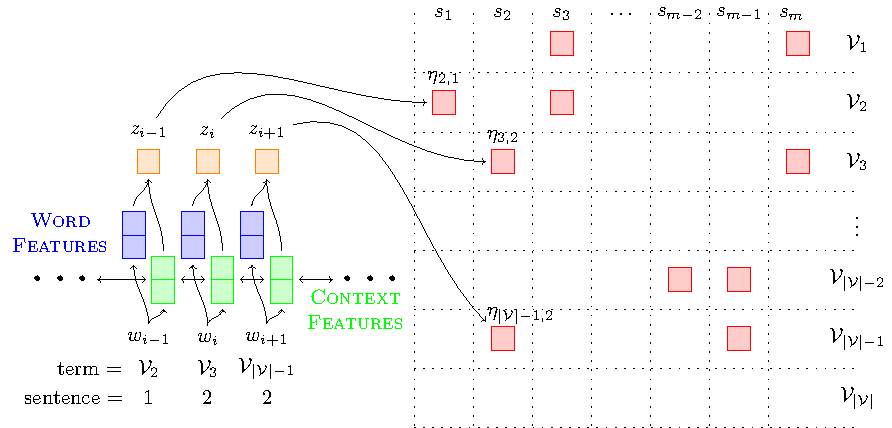
\includegraphics[scale=1.0]{dl_based_salience_models/figures/4_2_wimp_model.pdf}
 \end{center}
 \caption{(Left) Word and context features are extracted from the flat token
sequence representation to get word level importance scores 
$\wordImportance_i$. (Right) Word level scores are aggregated into a sparse
bag-of-words matrix with rows and columns corresponding to sentences and 
words respectively.}
\end{figure}

Our previous experiments revealed that lexical sematics were not the 
main driver of learning in sentence extractive news summarization. 
One could plausibly argue that it is a feature, not a bug, and that 
the structural
signals in news are intentional and not to be avoided. However, we think more 
attention could be paid to estimating importance scores at the word level.
We are motivated by potential application to abstractive generation: better
word level importance estimation could help to remove all but the most 
necessary content from the documents as a preprocessing stage before
abstractive summarization. We are also encouraged by practices
in multi-document news summarization, where word importance weights 
are the main ingredient in sentence representations. 


\newcommand{\classy}{\textsc{Classy}}
\newcommand{\occams}{\textsc{Occams}}

%\subsubsection{A brief discussion of \mlingsys.}

\occams{} and its antecedent \classy{} have been consistent top performers in various
summarization workshops \citep{conroyback,conroyclassy,davis2012occams}. 
In general their main approach 
is to represent each sentence as a sparse bag-of-words, where non-zero
entries correspond to word importance weights for the words found in the 
sentence. Typically, tf-idf weights are used for the importance scores.
The term by sentence matrix representing the document or documents to be
summarized is then factorized into two  matrices (typically with
non-negative entries) representing term factors and sentence factors.
The entries in the sentence factor matrix represent latent ``topics,'' 
and apriori the importance of each sentence is the sum of its latent topic
entries.

Sentence selection can subsequently be performed using one of several methods.
In the naive case, one can select the sentence with the highest vector norm, 
substract the selected latent factors from the remaining sentence vectors
(zeroing out any terms that become negative), and repeating until the
summary length budget is reached. More sophisticated selection procedures
involving multi-dimensional knapsack packing or submodular optimization 
can be used, however these are not the focus of this work.

One draw back to this approach is that the sentence factors and word 
importance scores are unsupervised with respect to the final summarization
objective; their utility to the summarization task is a happy coincidence.
Additionally, the word importance scores are not assigned based on the 
context in which the word appears.

We propose to address these issues by learning word level importance 
scores in the process of single document sentence extractive summarization.
Additionally, we propose a method of adapting these scores from the 
single document case to multi-document summarization.

\subsubsection{Proposed Model}


%In our proposed model for word importance, we first run the \elmo{}model 
%\citep{peters2018deep}
%over the input document to obtain contextual representations
%of each word. The \elmo{}embeddings are then combined with pretrained
%\glove embeddings along with embeddings for document frequency, 
%topic signature,
%sentence position, and part-of-speech tag, and then
%fed into a multi-layer perceptron to predict a scalar importance score.
%When a word occurs multiple times in the input, it can be given a different 
%importance score at each location because the \elmo{} embeddings will capture
%contributions of the salient neighbor words. A term-sentence matrix is 
%then formed from the input, using the estimated word importance scores 
%as the term weights. A sentence extractive summary can be obtained 
%using the naive sentence selection method described above or in 
%\autoref{alg:wimp_ext_alg}.
%The total score for the summary can also be obtained.
%
%We can train this summarizer using a gold extract sequence and a margin loss
%\[\objective(\theta) = \max\big(0, 1 + f(\predSaliences; \theta) - f(\saliences; \theta) \big) \] where $f(\predSaliences;\theta)$ is
%the score of our predicted extract summary.
%
%
%Let $\bowvec_1, \bowvec_2, \dots, \bowvec_n$ be the bag of words 
%representations of the 
%sentences selected for the summary, in the order they were selected.
%The score for the summary is computed as computed by the simple selection
%procedure would be
%$f() = \sum_{i=1}^n \sum_{j=1}^k \max(0, z_{i,j} - \sum_{l=1}^{i-1} z_{l,j})$ 
%
%
%~\\
%~\\

Let $\vocab$ be a finite vocabulary of words. A document $\doc$
is a sequence of $m$ words $(\word_1, \word_2, \ldots, \word_m) \in \vocab^m$.
We define two mappings of words to dense vector representations.
The first $\fdef{\wordFeatures}{\vocab}{\Rn{n_f}}$ maps words to 
a concatenation of feature embeddings whose total dimension is of size $n_f$. 
The various components of the feature embeddings include the word's \glove{} 
embedding, as well as embeddings for sentence position, document frequency,
and other word features that have been shown to be useful for summarization.
The second mapping
$\fdef{\contextFeatures}{\vocab}{\Rn{n_c}}$ maps the word to it's contextual
embedding; here this corresponds to the output of \elmo{} 
\citep{peters2018deep} at that word's
position in the document. 
The importance score $\wordImportance_i$ of a word $\word_i$ is the output of 
a feedforward layer 
\[ \wordImportance_i = \sigma\Big(\mathbf{v}^T \left[\begin{array}{c} \wordFeatures(\word_i) \\ \contextFeatures(\word_i) \end{array} \right] + b \Big) \]
    where $\mathbf{v} \in \Rn{n_f + n_c}$ and $b \in \R$ are learned weight
and bias parameters, and $\sigma$ is the logistic sigmoid.

Next, we aggregate the flat token level scores $\wordImportance_i$ into a
bag-of-words (BOW) 
representation for each sentence in the document.
Let $I_i$ be the set of indices of the flat word sequence corresponding
to the words in $i$-th input sentence. Then, let $\bow_i$ be the BOW 
representation of the $i$-th sentence with entries 
\[ \bow_{i,j} = \begin{cases} 
    0 & \textrm{if $\word_k \ne \vocab_j $ for all $k \in I_i $} \\ 
\sum_{k \in I_i} \mathbbm{1}\{\word_k = \vocab_j \} \cdot \wordImportance_k  & \textrm{otherwise}     \end{cases} \]
        for all $j \in \{1, \ldots, |\vocab|\}$.



\begin{figure}
  \begin{algorithmic}[1]
      \Procedure{\textsc{BowExtracter}}{$\bow_{1:n}, \beta, \kappa$}
   
      \State $\bow_i^{(1)}  \gets \bow_i \quad \forall i \in \{1, \ldots, n\}$
      \State $\hat{\eta} \gets 0$
      \State $t \gets 0$
      \While{ $\sum_{i=1}^t \kappa_{\predLabels_i} < \beta$ and $t < n$}
        \State $t \gets t + 1$
        \State $\predLabels_t \gets \operatorname{arg max}_{i \in \{1,\ldots, n\}}
            \sum_{j=1}^{|\vocab|} \bow^{(t)}_{i,j}$
            \State $\bow_i^{(t+1)} \gets \max(0, \bow_i^{(t)} - \bow^{(t)}_{\predLabels_t} )\quad  \forall i \in \{1, \ldots, n \}$
        \State $\hat{\eta} \gets \hat{\eta} + \sum_{j=1}^{|\vocab|} \bow_{\predLabels_t,j}^{(t)}$
         

      \EndWhile
        \State \Return $[\predLabels_1,\ldots,\predLabels_t], \hat{\eta}$ \Comment{Returns summary sentence indices and summary score.}
    \EndProcedure
  \end{algorithmic}
\caption{Simple sentence extraction algorithm given
 the sentence BOW representations $\omega_i$, 
  a word budget $\beta$, and a vector $\kappa$ of sentence lengths (in words)
  as input.}
\label{alg:wimp_ext_alg}
\end{figure}



        With the BOW representations in hand, we perform sentence selection
        using the algorithm presented in \autoref{alg:wimp_ext_alg} to 
        obtain a predicted extract indices $\predLabels$ and their associated
        overall summary score $\hat{\eta}$.

        We can optimize this model using a margin loss, where given a 
        gold extract sequence  $\labels$, we can compute the associated
        gold extract summary score $\eta$ and then minimize the following
        loss function \[\mathcal{L}_{ext}(\predLabels, \labels;\theta) = \max\big(0, 1 + \hat{\eta} - \eta\big)\]
        with respect to the parameters $\theta$ of the word importance 
        predictor.
        If needed, we can also introduce a supervised learning signal to the 
        individual word importance scores by collecting labels $\zeta_i$ for
        each $\wordImportance_i$ such that $\zeta_i = 1$ if $\word_i$ occurs
        and any human reference abstract and $0$ otherwise. The 
        $\objective_{ext}$ would then be augmented with an additional cross
        entropy loss for the word level predictions:
        \[ \mathcal{L}_{word}(\wordImportance, \zeta; \theta) = -\sum_{i=1}^m \zeta_i \log \wordImportance_i + (1 - \zeta_i) \log (1 - \wordImportance_i). \] 




        \paragraph{Adaptation to MDS} We also propose a simple 
        self attention-based modification to
        the word importance aggregation step to help adapt this method
        to multi-document summarization (MDS). \cite{conroy2013multilingual} 
        found
        that dimensionality reduction on the BOW representations improves
        summarizer performance in the MDS setting (but not as much on
 single document
        summarization). 


        We plan to experiment with the following importance 
        aggregation method. First, given the outputs of the contextual features
        $\mathbf{h}_i = \contextFeatures(\word_i)$, 
        we compute a self attention matrix $\Lambda \in \Rn{m\times m}$
        where \[\Lambda_{i,j} = \sigma(\mathbf{h}_i^T \mathbf{h}_j / \tau + b)  \]
        using sigmoidal attention \citep{kim2017structured} with a learned bias 
        parameter $b$ and a temperature parameter $\tau$.
        Next we compute an attention weighted word importance score $\bar{\wordImportance}_i$ for each word in the input using the following formula,
        \[ \bar{\wordImportance}_i = \sum_{j=1}^m \wordImportance_j \cdot \Lambda_{i,j}.\]
        We then use the aggregated word importance scores 
    $\bar{\wordImportance}_i$ inplace of their nonaggregated counterparts
        in the creating the BOW representations $\omega_j$.

        Our motivation is that by accumulating scores based on context
        similarity, words and topics that appear in multiple documents 
        will accumulate the bulk of the word importance scores, giving 
        an added boost to sentences that contain them. Implicitly, errant
        words from one document that are not on topic to the cluster will
        effectively not contribute much to a sentences score, reducing the 
        effectve dimension of the BOW vectors and regularizing individual
        sentences to the document cluster's mean.

        
        Since we are training our models on single documents, we expect that
        running our pretrainined word scoring model on the individual 
        documents from an MDS document cluster will result in 
        minimal task-adaptation mismatch. The remaining bias and temperature
        parameters can easily be tuned on the small amount of MDS training 
        data available.

%        We also plan to compare this method to using a non-negative matrix 
%        factorization 
%        method on the output of the learned BOW representation, 
%        and to hard attention assignments using Brown clustering.







%\subsubsection{
%\cite{conroy} 


 


%
\subsection{Deep Learning Models of Sentence Salience}

\begin{frame}{Summarizer Architecture}
  \begin{center}
    \begin{tikzpicture}
      \node at (0.4,-.75) {Sentence 1};
      \node at (4.9,-.75) {Sentence 2};
      \node at (8.9,-.75) {Sentence 3};
      \node (w1) at (0,0) 
      {\large $\uncover<2->{\textsc{Enc}\left(}w^{(1)}_1,
         w^{(1)}_2, w^{(1)}_3\uncover<2->{\right)}$};

      \node (w2) at (4.5,0) 
      {\large $\uncover<2->{\textsc{Enc}\left(}w^{(2)}_1, 
         w^{(2)}_2, w^{(2)}_3\uncover<2->{ \right)}$};
      \node (w3) at (8.6,0) 
      {\large $\uncover<2->{\textsc{Enc}\left(}w^{(3)}_1, 
         w^{(3)}_2\uncover<2->{\right)}$};

      \node (s1) at (3,2) {\large $\uncover<3->{s_1}$};
      \node (s2) at (4,2) {\large $\uncover<3->{s_2}$};
      \node (s3) at (5,2) {\large $\uncover<3->{s_3}$};
      \uncover<3->{  
        \draw[->,thick] (w1.north) -- (s1.south); 
        \draw[->,thick] (w2.north) -- (s2.south);
        \draw[->,thick] (w3.north) -- (s3.south);
      }

      \uncover<4->{
        \node (ext) at (3.6,2) {\large $\textsc{Ext}\Big( 
        \quad\quad\quad\;\;\;\;\;\;\;\;\;\;\; \Big)$};
      }
      \uncover<5->{
        \node (y1) at (3,3.5) {\large $y_1$};
        \node (y2) at (4,3.5) {\large $y_2$};
        \node (y3) at (5,3.5) {\large $y_3$};
        \draw[->,thick] (s1.north) -- (y1.south);
        \draw[->,thick] (s2.north) -- (y2.south);
        \draw[->,thick] (s3.north) -- (y3.south);
      }

    \end{tikzpicture}
  \end{center}
\end{frame}


\begin{frame}{Sentence Encoders}
 \begin{columns}[t]
  \column{.32\textwidth}
   \centering
   Averaging Encoder\\~\\
   \includegraphics[]{images/section3/avg_encoder.pdf}\\
  \column{.32\textwidth}
   \centering
   RNN Encoder\\~\\
   \includegraphics[]{images/section3/rnn_encoder.pdf}\\
  \column{.32\textwidth}
   \centering
   CNN Encoder\\~\\
   \includegraphics[]{images/section3/cnn_encoder.pdf}\\
 \end{columns}

~\\
We use pretrained (Wikipedia/Gigaword) Glove word embeddings.

\end{frame}
%
%\begin{frame}{Sentence Extractor}
%  \textbf{Previous Work}\\~\\
%  ~~ -- \textbf{Cheng and Lapata Extractor} ~~ seq2seq inspired architecture 
%                                               (Cheng and Lapata, 2016)\\
%  ~~ -- \textbf{SummaRunner Extractor} ~~ RNN inspired architecture with 
%                                          document and summary representations 
%                                          (Nallapati et al., 2016)\\
%  ~\\~\\
%  \textbf{Our Extractors}\\~\\
%  ~~ -- \alert<2>{\textbf{RNN Extractor}} ~~ Simplified version of SummaRunner \\
%  ~~ -- \textbf{Seq2Seq Extractor} ~~ seq2seq (with attention) inspired 
%                                      architecture \\
%\end{frame}


\begin{frame}{Sentence Extractors}
 \begin{columns}[t]
  \column{.4\textwidth}
  \only<1,2,4>{
   \centering
   SummaRunner Extractor\\
   (Nallapati et al. 2016)\\
   \includegraphics[scale=.65]{images/section3/sr_extractor.pdf}\\
   RNN Extractor (ours)\\
   \includegraphics[scale=.65]{images/section3/rnn_extractor.pdf}
}
\only<3>{
    Cheng \& Lapata Model
    \begin{enumerate}
        \item Offset encoder/decoder inputs, no attention
        \item Complex interaction between previous extraction prediction and 
            decoder input.
    \end{enumerate}
    ~\\~\\
    Seq2Seq Model
    \begin{enumerate}
        \item Simple dot-product attention
        \item \textbf{(Conditionally) independent} extraction decisions
    \end{enumerate}
}
  \column{.6\textwidth}
  \only<1,3,4>{
   \centering
   Cheng \& Lapata Extractor\\
   (Cheng and Lapata, 2016)\\
   \includegraphics[scale=.65]{images/section3/cl_extractor.pdf}\\
   Seq2Seq Extractor (ours)\\
   \includegraphics[scale=.65]{images/section3/s2s_extractor.pdf}
   }
   \only<2>{
        SummaRunner Model
        \begin{itemize}
        \item Internal representations of document similarity and summary novelty
        \item Explicit representation of position
        \item Complex dependencies between extraction decisions
        \end{itemize}
~\\
~\\
        RNN Model
        \begin{itemize}
            \item \sout{Internal representations of document similarity and summary novelty}
            \item \sout{Explicit representation of position}
            \item \textbf{(Conditionally) independent} extraction decisions
        \end{itemize}

   }
 \end{columns}

\end{frame}


\begin{frame}{Experiments}
%
    \alert<4>{\textbf{Main Experiment}}\\
    Evaluate encoder/extractor pairs using ROUGE-2 recall.\\
%
  \begin{columns}
    \begin{column}{0.3\textwidth}
    \uncover<5->{\textbf{Additional Experiments}}    
      \begin{itemize}
        \uncover<5->{\item \alert<5>{fine-tuned embeddings}}
        \uncover<6->{\item \alert<6>{word class ablations}}
        \uncover<7->{\item \alert<7>{sentence order shuffling}}
      \end{itemize}
    \end{column}
    \begin{column}{0.7\textwidth}
        \begin{tikzpicture}[thick,scale=0.7, every node/.style={transform shape}]

  \draw[draw=black] (-2,5) rectangle (10.1,-2.5);

  \uncover<1-6>{
    \node (w1) at (0,0) 
      {\large $\textsc{Enc}\left(w^{(1)}_1,
       \uncover<-5,7->{w^{(1)}_2,} w^{(1)}_3\right)$};
    \node (w3) at (8.6,0) 
      {\large $\textsc{Enc}\left( \uncover<-5,7->{ w^{(3)}_1, }
       w^{(3)}_2 \right)$};
    \node (w2) at (4.5,0) 
      {\large $\textsc{Enc}\left(w^{(2)}_1, 
       w^{(2)}_2,\uncover<-5,7->{  w^{(2)}_3} \right)$};


  }
  
  \uncover<7>{
    \node (w21) at (0,0) 
      {\large $\textsc{Enc}\left(w^{(2)}_1, w^{(2)}_2,w^{(2)}_3 \right)$};
    \node (w13) at (8,0) 
      {\large $\textsc{Enc}\left(w^{(1)}_1, w^{(1)}_2, w^{(1)}_3\right)$};
    \node (w32) at (4,0) 
      {\large $\textsc{Enc}\left(w^{(3)}_1, w^{(3)}_2 \right)$};
  }





  \uncover<1-6>{
    \node (s1) at (3,2) {\large $s_1$};
    \node (s2) at (4,2) {\large $s_2$};
    \node (s3) at (5,2) {\large $s_3$};
  }
  \uncover<7>{
    \node (s13) at (5,2) {\large $s_1$};
    \node (s21) at (3,2) {\large $s_2$};
    \node (s32) at (4,2) {\large $s_3$};
  }


    \draw[->,thick] (w1.north) -- (s1.south); 
    \draw[->,thick] (w2.north) -- (s2.south);
    \draw[->,thick] (w3.north) -- (s3.south);

    \node (ext) at (3.6,2) {\large $\textsc{Ext}\Big( 
        \quad\quad\quad\;\;\;\;\;\;\;\;\;\;\; \Big)$};
\uncover<2->{
    \node (extp) at (-.8,2) {\large $\theta_\textsc{Extractor}$};
    \node (encp) at (5.5,-2) {\large $\theta_\textsc{Encoder}$};
    \draw[->,thick] (encp.north) -- (w1.south);
    \draw[->,thick] (encp.north) -- (w2.south);
    \draw[->,thick] (encp.north) -- (w3.south);
    \draw[->,thick] (extp.east) -- (ext.west);
}

\uncover<3->{
    \node (embp) at (2.5,-2) {\large $\theta_\textsc{Embeddings}$};
    \draw[->,thick] (embp.north) -- (w1.south);
    \draw[->,thick] (embp.north) -- (w2.south);
    \draw[->,thick] (embp.north) -- (w3.south);
}
\uncover<4->{
        \draw[draw=red] (extp.north east) rectangle (extp.south west);
       \draw[draw=red] (encp.north east) rectangle (encp.south west);
    \node (glovep) at (-1,-2) {\large $\theta_\textsc{Glove}$};
    \draw[->,thick] (glovep.east) -- (embp.west);

}
\uncover<5>{
        \draw[draw=red] (embp.north east) rectangle (embp.south west);
}
    \node (y1) at (3,3.5) {\large $y_1$};
    \node (y2) at (4,3.5) {\large $y_2$};
    \node (y3) at (5,3.5) {\large $y_3$};
    \draw[->,thick] (s1.north) -- (y1.south);
    \draw[->,thick] (s2.north) -- (y2.south);
    \draw[->,thick] (s3.north) -- (y3.south);

    \node (loss) at (4, 4.5) {\large \textsc{Loss}};
    \draw[->,thick] (y1.north) -- (loss.south);
    \draw[->,thick] (y2.north) -- (loss.south);
    \draw[->,thick] (y3.north) -- (loss.south);
 

%    \uncover<2->{   
 %      \draw[->,thick,red] (loss.south) + (-5mm, 0) -- (y1.north west);
 %      \draw[->,thick,red] (loss.south) + (5mm, 0) -- (y3.north east);
 %   }
 %   \uncover<3->{
 %      \draw[->,thick,red] (y1.north west) -- (s1.north west);
 %      \draw[->,thick,red] (y3.north east) -- (s3.north east);
 %   }
 %   \uncover<4->{
 %      \draw[->,thick,red] (s1.north west) -- (extp.north east) ;
 %   }
 %   \uncover<5->{
 %      \draw[->,thick,red] (s1.south west)+(-5mm,0) -- (-.7, .6) ;
 %      \draw[->,thick,red] (s3.south east)+(5mm,0) -- (9.2, .6) ;
 %   }
%    \uncover<6->{
 %      \draw[->,thick,red] (-.7, -.5) -- (encp.north west) ;
 %      \draw[->,thick,red] (9.2, -.5) -- (encp.north east) ;
 %      \draw[->,thick,red] (w2.south)+(-2mm,0) -- (4.3, -1.5) ;
  %  }
    

\end{tikzpicture}
 
    \end{column}
  \end{columns}
\end{frame}

\begin{frame}{Model Training}

    Maximum Likelihood training using gold extract summaries.

    \[\max_{\theta} \frac{1}{|\mathcal{D}|} \sum_{(s,y^*)\in \mathcal{D}} 
    \log p(y^*| s) \]

   
    ~\\
    ~\\
    ~\\

    Gold extract summaries $y^*$ created by greedily selecting the sentences that maximize ROUGE, as in Nallapati et al. (2016).

\end{frame}

\begin{frame}{Summary Generation}

    \begin{enumerate}
        \item Rank sentences $s_i$ in decreasing order by $p(y_i=1|h)$.
            ~\\~\\
            ~\\~\\


        \item Create a summary by extracting the top ranked sentences until a word length budget.
    \end{enumerate}

\end{frame}



\begin{frame}{Choice of Sentence \textbf{Encoder}: News}
  \begin{center}
      \begin{tabular}{ccgcg} 
        & & \multicolumn{3}{c}{\textbf{Rouge-2 Recall}}\\
      \toprule
      \textbf{\textsc{Ext}} & \alert{\underline{\textbf{\textsc{Enc}}}}
          & \textbf{CNN/DM} & \textbf{NYT} & \textbf{DUC} \\
      \midrule
      \textsc{Lead}   
         & --         &        $24.4$ &        $32.3$ &   $21.5$  \\
      \hline 
      \multirow{3}{*}{\textsc{Seq2Seq}}
         &\textsc{Avg}&
           \alert{\textbf{25.6}}&\textbf{35.7}&\alert{\textbf{22.8}}  \\
         &\textsc{Rnn}&        25.3 &\textbf{35.9}&        22.5   \\
         &\textsc{Cnn}&        25.1 &        35.1 &\textbf{22.7}  \\
         \hline
      \multirow{3}{*}{\textsc{Cheng \& Lapata}}
         &\textsc{Avg}&
           \alert{25.3}&\textbf{35.6}&\alert{\textbf{23.1}}\\
         &\textsc{Rnn}&        
                     25.0 &          \textbf{35.8} &          \textbf{23.0} \\
         &\textsc{Cnn}&       
                     25.1 &                  35.0  &          \textbf{23.0} \\
         \hline
      \textsc{Oracle} 
         & --         &          36.2 &        48.9 &        31.8   \\
      \bottomrule
    \end{tabular}
    
  \end{center}
  ~\\

  Averaging is either the \alert{\textbf{best}} encoder or 
  \textbf{statistically indistinguishable} from the best encoder!

\end{frame}

\begin{frame}{Choice of Sentence \textbf{Encoder}: Non-News}
  \begin{center}
    \begin{tabular}{ccgcg} 
        & & \multicolumn{3}{c}{\textbf{Rouge-2 Recall}}\\
  \toprule
  \textbf{\textsc{Ext}} & \alert{\underline{\textbf{\textsc{Enc}}}}
      & \textbf{Reddit} & \textbf{AMI} & \textbf{PubMed} \\
  \midrule
  \textsc{Lead}   
     & --         &        $\mathbf{10.9}$ &        $2.0$ &   $9.3$  \\
  \hline
  \multirow{3}{*}{\textsc{Seq2Seq}}
     &\textsc{Avg}&
                   \alert{\textbf{13.6}}&\alert{\textbf{5.5}}&\alert{\textbf{17.7}} \\
     &\textsc{Rnn}&
                   \textbf{12.0}&\textbf{5.3}&        16.7  \\
     &\textsc{Cnn}&
                   \textbf{13.2}&        2.9&        16.9  \\
     \hline
  \multirow{3}{*}{\textsc{Cheng \& Lapata}}
     &\textsc{Avg}&
       \alert{\textbf{13.6}} & \alert{\textbf{6.1}}   & \alert{\textbf{17.7}}\\
     &\textsc{Rnn}&       
       \textbf{12.6} & \textbf{5.0}   & 16.7\\
     &\textsc{Cnn}&       
       \textbf{13.4} & 2.8               &  16.9      \\
     \hline
  \textsc{Oracle} 
     & --         &       16.2    &    3.9     &       25.0   \\
  \bottomrule
\end{tabular}

    
  \end{center}
  ~\\

  Averaging is either the \alert{\textbf{best}} encoder or 
  \textbf{statistically indistinguishable} from the best encoder!
\end{frame}

\begin{frame}{Choice of Sentence \textbf{Extractor}: News}
    
 \begin{center}
   \begin{tabular}{ccgcg}
 & & \multicolumn{3}{c}{\textbf{Rouge-2 Recall}}\\
 \toprule
 \alert{\underline{\textbf{Ext}}} & \textbf{Enc} & 
   \textbf{CNN/DM} & \textbf{NYT} & \textbf{DUC} \\
 \midrule
 \textsc{Lead}    &  --          & 
                   24.4  & 32.3  & 21.5 \\
 \hline
 \textsc{RNN}     & \textsc{Avg} &  
                   25.4  & 34.7  & 22.7 \\
 \hline
 \textsc{Seq2Seq} & \textsc{Avg} & 
           \alert{\textbf{25.6}} & \alert{\textbf{35.7}} & \textbf{22.8} \\
 \hline
 \textsc{Cheng \&  Lapata} & \textsc{Avg} & 
                    25.3 & \textbf{35.6} & \textbf{23.1} \\
 \hline
 \textsc{SummaRunner}  & \textsc{Avg} &  
                    25.4 & 35.4 & 22.3 \\
 \hline
    \textsc{Oracle} & -- & 36.2 &  48.9 &  31.8\\
 \bottomrule
\end{tabular}

 \end{center}
 
 ~\\

 \textsc{Seq2Seq} is the \alert{\textbf{best}} or \textbf{statistically 
 indistinguishable} from the best system.

 ~\\
 \textsc{Rnn} extractor as good as \textsc{SummaRunner} or 
 \textsc{Cheng \& Lapata} extractors on CNN/DailyMail data.

  

\end{frame}

\begin{frame}{Choice of Sentence \textbf{Extractor}: Non-News}
    
 \begin{center}
   \begin{tabular}{ccgcg}
 & & \multicolumn{3}{c}{\textbf{Rouge-2 Recall}}\\
\toprule
\alert{\underline{\textbf{Ext}}} & \textbf{Enc} & 
   \textbf{Reddit} & \textbf{AMI} & \textbf{PubMed} \\
\midrule
\textsc{Lead}    &  --          & 
                   \textbf{10.9}  & 2.0  & 9.3 \\
\hline
\textsc{Rnn}     & \textsc{Avg} &  
                   \textbf{11.4}  & \textbf{5.5}  & 17.0 \\
\hline
\textsc{Seq2Seq} & \textsc{Avg} & 
           \alert{\textbf{13.6}} & \textbf{5.5} & \textbf{17.7} \\
\hline
\textsc{Cheng \&  Lapata} & \textsc{Avg} & 
           \textbf{13.6} & \textbf{6.1} & \textbf{17.7} \\
\hline
\textsc{SummaRunner}  & \textsc{Avg} &  
           \textbf{13.4} & \textbf{5.6} & \textbf{17.2} \\
\hline
    \textsc{Oracle} & -- & 16.2 &  3.9 &  25.0\\
\bottomrule
\end{tabular}


 \end{center}

 ~\\

 \textsc{Seq2Seq} is the \alert{\textbf{best}} or \textbf{statistically indistinguishable} from the best
 system.


\end{frame}



\begin{frame}{Word Embedding Fine-Tuning: (News)}
  \begin{center}
    \begin{tabular}{ccccc}
      & & \multicolumn{3}{c}{\textbf{Rouge-2 Recall}}\\
      \toprule
        \textbf{Ext} & \textbf{Emb}  & 
           \textbf{CNN/DM} & 
           \textbf{NYT} & 
           \textbf{DUC} \\
      \midrule
      \multirow{2}{*}{\textsc{Seq2Seq}} 
        & Fixed & \textbf{25.6} & \textbf{35.7} & \textbf{22.8} \\
        & Fine-Tuned &         25.3  & \textbf{35.7} & \textbf{22.9} \\
      \hline
      \multirow{2}{*}{\textsc{Cheng \& Lapata}} 
        & Fixed & \textbf{25.3} & \textbf{35.6} & \textbf{23.1} \\
        & Fine-Tuned &         24.9  &         35.4  & \textbf{23.0} \\
      \bottomrule
  \end{tabular}


 \end{center}

 ~\\
 
% Performance difference when using \textit{fixed} embeddings versus 
% \textit{fine-tuned} embeddings.
 
  ~\\

%  Models are using the \textsc{Avg} encoder and are initialized with 
%  Glove embeddings. 

%  ~\\

  \textbf{No statistically significant improvement} on news with fine-tuning!

\end{frame}

\begin{frame}{Word Embedding Fine-Tuning: Non-News}
 \begin{center}
  \begin{tabular}{ccccc}
   & & \multicolumn{3}{c}{\textbf{Rouge-2 Recall}}\\
   \toprule
   \textbf{Ext} & \textbf{Emb}  & 
        \textbf{Reddit} & \textbf{AMI} & \textbf{PubMed} \\
   \midrule
   \multirow{2}{*}{\textsc{Seq2Seq}}
      & Fixed & \textbf{13.6} &         5.5  & \textbf{17.7} \\
      & Fine-Tuned & \textbf{13.8} & \textbf{5.8} &         16.9  \\
   \hline
   \multirow{2}{*}{\textsc{Cheng \& Lapata}} 
      & Fixed & \textbf{13.6} & \textbf{6.1} & \textbf{17.7} \\
      & Fine-Tuned & \textbf{13.4} & \textbf{6.2} & \textbf{16.4} \\
   \bottomrule
  \end{tabular}


 \end{center}

 ~\\
 
% Performance difference when using \textit{fixed} embeddings versus 
% \textit{fine-tuned} embeddings.
 
 ~\\

% All models are using the \textsc{Avg} encoder and are initialized with 
% pretrained Glove embeddings from gigaword/wikipedia. 

% ~\\
 \textbf{Statistically significant improvement} with \textsc{Seq2Seq} on AMI
 data. (Caveat: only speech dataset)\\

~\\
Otherwise, same trend as news, \textbf{no stat. sig. improvement} using fine-tuning.

\end{frame}

\begin{frame}{Word Class Ablation: ROUGE-2 Recall}
 \begin{center}
  \begin{tabular}{lcccccc}
   \toprule
   \multirow{1}{*}{\textbf{Ablation}} & 
            \textbf{CNN/DM} & \textbf{NYT} & \textbf{DUC} &
            \textbf{Reddit} & \textbf{AMI} & \textbf{PubMed} \\
   \midrule
     All Words & $\mathbf{25.4}$ & $\mathbf{34.7}$ & $22.7$ &
                  $\mathbf{11.4}$ & $5.5$ & $\mathbf{17.0}$  \\
   \uncover<2->{$-$ Nouns & $25.3$  & $34.3 $ & $22.3$  &
   \alert<2>{$10.3$} & \alert<2>{$3.8$} & \alert<2>{$15.7$}} \\
   \uncover<2->{$-$ Verbs & $25.3$  & $34.4 $ & $22.4$ &
            $10.8$ & $5.8$ & $16.6$ }\\
   \uncover<3->{$-$ Adj/Adv & 
  $25.3$ & $34.4$ & $22.5$ &
   \alert<3>{$9.5$} & $5.4$ & $16.8$} \\
   \uncover<4->{$-$ Function & $25.2$ & $34.6$ & \alert<4>{$\mathbf{22.9}$} &
   $10.3$ & \alert<4>{$\mathbf{6.3}$} & $16.6$ }\\
   \bottomrule
  \end{tabular}
 \end{center}


 %RNN extractor with Averaging encoder. 

 %~\\


 \uncover<2->{\textbf{-Nouns/Verbs} Doesn't decrease performance much on News. Non-News sees small performance drops. }

~\\ 

 \uncover<3->{\textbf{-Adj/Adv} Intensifiers are important in personal stories.
 Signal climactic and important moments.}


 ~\\

 \uncover<4->{\textbf{-Function} Possibly noisy signals on small datasets.}



 ~\\
 \uncover<1-5>{\tiny{\textbf{Bold} is best performance.}}

\end{frame}



\begin{frame}{Shuffled vs In-Order (News)}

 \begin{center}
  \begin{tabular}{ccL{2cm}m{1cm}L{.75cm}} 
   \toprule
   \textbf{Ext.} & \textbf{Order} & 
                           \textbf{CNN/DM} & \textbf{NYT} & \textbf{DUC} \\
   \midrule
%?   \multirow{2}{*}{RNN} 
%?       & In-Order & 
%?       \textbf{25.4} & \textbf{34.7} & \textbf{22.7} \\
%?       & Shuffled & 
%?               22.8 &          25.0  &         18.2  \\
   \multirow{2}{*}{Seq2Seq}
       & In-Order & 
       \textbf{25.6} & \textbf{35.7} &  \textbf{22.8} \\
       & Shuffled & 
               21.7  &         25.6  &          21.2  \\
   \bottomrule
  \end{tabular}
 \end{center}

 ~\\

 Shuffled model is trained on shuffled sentence order documents.

 ~\\

 Both models evaluated on in-order data.


~\\ 
 Large \textbf{performance drops} on news!

\end{frame}

\begin{frame}{Shuffled vs In-Order (Other)}

 \begin{center}
  \begin{tabular}{ccccc} 
   \toprule
   \textbf{Ext.} & \textbf{Order} & 
                           \textbf{Reddit} & \textbf{AMI} & \textbf{PubMed} \\
   \midrule
   \multirow{2}{*}{Seq2Seq}
       & In-Order & 
       \textbf{13.6} &         5.5  &  \textbf{17.7} \\
       & Shuffled & 
       \textbf{13.5} & \textbf{6.0} &          14.9  \\
   \bottomrule
  \end{tabular}
 \end{center}

 ~\\

 Shuffled model is trained on shuffled sentence order documents.

 ~\\

 Both models evaluated on in-order data.

 ~\\

 Small \textbf{performance increase} on AMI.

\end{frame}



%\input{3_2_deep_learning_word_salience.tex}

\section{Deep Learning Models of Content Salience}
\label{sec:chapter4}
\label{sec:deep_learning_salience}


Increasingly, deep neural 
network models are being used to perform sentence extractive summarization 
tasks. While these models are very flexible and allow for easy hierarchical 
representation learning, it is unclear what signals they are extracting
from the data to make predictions.
In this section, we describe our completed experiments teasing out the 
importance
of different neural network designs for sentence level salience estimation
\citep{kedzie2018deep}. 
In particular, we experiment with several methods for encoding a sequence
of word embeddings into a sentence embedding, and then in turn, mapping
a sequence of sentence embeddings to sentence salience predictions. We 
introduce several simplifications to existing models in the literature, and
show their effectiveness on an SDS task across news, personal narratives,
workplace meetings, and medical journal article genres.

We also perform several diagnostic experiments 
and find impediments to learning robust models of 
sentence salience. In particular, the sentence position implicitly 
encoded in the models dominates the learning signal. While sentence position
is certainly an important feature in news, not all domains or tasks 
will share this feature;
 we would also like to be able to design
models that make their salience decisions primarily on lexical or
topical content.

We believe that the sentence embedding representation is too coarse to
make significant use of lexical information in the presence of less noisy
position features, even when position is only implicitly represented by 
the model.
To that end, we propose a new deep learning based SDS model that directly 
estimates individual word level salience scores, and a simple sentence 
selection and margin loss framework for learning. In this model,
we augment the word embeddings (which only capture shallow lexical semantics)
with embeddings representing other word features. Our initial experiments
suggest that document frequency, and information theoretic accounts of 
surprisal (e.g. topic signatures) are also useful for the summarization task. 
We expect to show less dependence on the position features using
the same ablation diagnostics we applied to our sentence level salience 
models. 
While previous work has estimated word importance using these features
in a linear model 
\citep{hong2014improving}, they were only able to take limited advantage of 
context features, i.e. taking a weighted average of word features to
the left and right. By contrast,
 in our proposed model we can combine rich
document specific contextual features, e.g. \textsc{Elmo} embeddings 
\citep{peters2018deep}, in conjunction with these word features.

Additionally, we plan to adapt this word level salience model to a news MDS task;
if it is less dependent on sentence position, it should be more amenable 
to MDS where lexical centrality to the document cluster is possibly
the dominant learning signal.  
%We concluded this section with proposed domain adaptation experiments for
%modifying the word importance model to work on a news MDS task. 
The MDS version of the model will use an importance score aggregation step
where word level scores accrue additional importance across documents 
using an attention mechanism.


In the next subsections we first briefly cover related work on sentence
and word level salience estimation before covering the 
completed sentence level
and proposed word level salience estimation experiments.
%are the
%This
%work describes impedements to learning and word and sentence representations
%in deep learning models of extractive summarization, and led to 
%a recent publication \citep{kedzie2018deep}. Based on these limitations,
%we propose extensions to the word level representations and explicitly model
%word level salience scores as a means to performing sentence extractive
%summarization. While the finished and proposed work focuses on single document
%summarization, we also propose an extension of the word level salience
%estimation model that we hope will generalize to the multi-document
%summarization context.















\subsection{Related Work}

Estimating sentence salience for summarization has often been approached as a 
sentence
classification problem. Na{\"i}ve Bayes 
\citep{kupiec1995trainable,teufel1997sentence,osborne2002using}, 
maximum entropy 
\citep{osborne2002using}, and support vector machine \citep{hirao2002ntt}
classifiers have all been applied to predict whether a sentence should
be included in an extract summary.
Sentence position features were a strongly predictive signal in all of these 
works.
Lexical features were more varied in their use; e.g., 
\cite{kupiec1995trainable} 
checked for the presence of key phrases from a manually curated list,
 \cite{osborne2002using} experimented with automatically extracted
bigram features, 
%of which only a small portion are actually discriminative,
while \cite{hirao2002ntt} used average \tfidf{} weights to capture
important lexical content.

While the previous works all estimated sentence salience independently,
a variety of structured prediction methods have also been explored
to jointly estimate the salience of sentences in a document or 
document cluster.
These include
hidden Markov models (HMMs) \citep{conroy2001text}, conditional random fields
(CRFs)
\citep{shen2007document}, large margin classifiers \citep{martins2009summarization}, and 
structured support vector
machines 
\citep{berg2011jointly,sipos2012large,durrett2016learning}. 
While positional or discourse features are important to all of these methods, 
\cite{martins2009summarization}, \cite{berg2011jointly}, and \cite{durrett2016learning} 
also learn lexical feature weights as part of their larger model.
Graph random walk based ranking has been another
prominent method for estimating salience of a collection of sentences 
jointly 
\citep{erkan2004lexrank,mihalcea2004textrank};
typically the sentence graphs are constructed using the cosine similarity
between a sentence's \tfidf{} weighted bag-of-words although other methods
of weighting graph edges have been used. Additionally, independent
sentence level priors about salience can also be incorporated by adjusting the 
probability of restarting the random walk \citep{erkan1001using,liu2008personalized}.


Deep learning methods have become the \textit{de facto} standard approach to many 
NLP problems, especially when there exists plentiful labeled data.
There has been a flurry of recent work on sentence extractive 
single document summarization of news using a variety of neural network 
architectures 
\citep{cheng2016neural,nallapati2016classify,nallapati2016summarunner,narayan2018ranking}.
These models have hierarchical representations of the document, using
either
recurrent neural networks (RNNs) or convolutional neural networks (CNNs)
to encode word embeddings into sentence embeddings which are then fed into
an RNN based sentence extractor. 
Unlike prior structured approaches,
finding the optimal label sequence in these models is intractable. However,
the richer word and sentence representations often yield better performance
even with a simpler inference method. 



%thanks in part to the availibilty of a large corpus 
%(approximately 300k) of CNN and Daily Mail articles with human written bullet 
%point summaries \citep{hermann2015teaching}.
%These models have typically built hierarchical representations of the text


%Comparing models and defining best practices for model design has become 
%difficult as papers often propose complex models with a variety
%of design choices, making it difficult to determine what choices actually
%lead to the best performance. 



There is also prior  work on estimating word importance directly 
(as opposed to learning word weights as a means to estimate sentence salience).
%Much of the summarization literature does not learn word importance weights, 
%but rather uses frequency derived proxies of importance instead 
%\citep{conroy2001text,shen2007document,sipos2012large,nenkova2005impact}.
%Other research has focused specifically on learning word importance weights
%directly. 
For example, \cite{yih2007multi} learn to predict the likelihood
of a term appearing in a summary using a maximum entropy classifier with
several document frequency and position features. \cite{hong2014improving}
extend these features to consider word type (e.g. named-entity type),
background information like the probability of the word occurring 
in a large collection of New York Times abstracts, and whether or
not the word occurs in an automatic summary (using an unsupervised summary
method). There does not appear to be much literature on extending this work
with deep learning, a gap we hope to fill with our proposed word level model. 
Outside of summarization,
\cite{sheikh2016learning} found that learning importance scores for 
words in a weighted bag-of-words model outperformed \tfidf{} based approaches
to text classification tasks like 
sentiment and topic detection. 
 


 



\subsection{Deep Learning Models of Sentence Salience}

 Given the diversity of neural architectural choices, a best practices
for sentence extracive summarization has yet to emerge. In this section
we ask what architecture design choices matter for single document 
summarization across a variety of domains.

We begin by definining some terminology. A sentence is represented as an
sequence of words $\sent = \word_1, \word_2, \ldots, \word_{|\sent|},$
where each word is drawn from a finite vocabulary $\vocab$ and $|\sent|$ is
the length of sentence $\sent$ in words. Similarly, a document $\doc =  
\sent_1, \sent_2, \ldots, \sent_{|\doc|} $ is a sequence of sentences, where 
$|\doc|$ is the size of the document in sentences.  

We treat sentence extractive summarization as a sequence tagging
problem: given a document $\doc$, we want to assign an associated binary
tag sequence $\Labels \in \{0,1\}^{\Sze{\doc}}$ such that the corresponding
set of extracts $\extracts = \{\sent_i \in \doc \; | \; \Labels_i =1 \}$ is
a suitable summary
of the document. Typically, it is assumed that the size of the extract summary
in sentences is much smaller than the input document, i.e. 
$|\extracts|  \ll |\doc|$.
It is also common to enforce a word budget $\budget$ such that
$\sum_{\sent \in \extracts} |\sent| \le \budget$.

A typical deep learning model will build up a hierarchical representation
of each sentence, starting at the word level, and then composing an arbitrarily
long sequence of word representations into a fixed length sentence 
representation.
First the individual words are 
projected to fixed length vectors, or word embeddings, via a mapping
$\embproj : \vocab
\rightarrow \mathbb{R}^{\embsize}$. The sentence encoder network $\encoder :
\{\mathbb{R}^{\embsize}\}^* \rightarrow \mathbb{R}^{\sembsize}$ is then 
responsible for mapping word embedding sequences to fixed length sentence 
embeddings. Finally, the sentence extractor network $\extractor : 
\{\mathbb{R}^\sembsize\}^* \rightarrow \{0, 1\}^*$ produces a label 
sequence $\Labels$.

We explore several choices of encoder and extractor architecture from the 
literature \citep{cheng2016neural,nallapati2016summarunner} as well as 
propose our own designs \citep{kedzie2018deep}. In the next sections,
we describe the different encoder and extractor architectures, before 
discussing data, experiments, and evaluation.

%the three sentence encoder architectures (\enAvg, 
%\enRnn, and \enCnn) followed by four extractor architectures 
%(\textit{rnn}, \textit{seq2seq}, \textit{sr}, and \textit{cl}).

\subsubsection{Sentence Encoders}
\paragraph{Averaging} This encoder simply averages a sentence's
associated word embeddings:
\[ \encoder_{avg}(\sent) = \frac{1}{|\sent|} \sum_{\word \in \sent} \embproj(\word). \]
Other than the word embeddings, this encoder involves no learned parameters,
and while it collapses word order, embedding averaging has consistently
been found competitive with more sophisticated sentence embedding techniques
\citep{iyyer2015deep,wieting2015towards,arora2016simple,wieting2017revisiting}.


\paragraph{Recurrent Neural Networks} The second encoder architecture
we experiment with is a recurrent neural network (RNN) over the word
embeddings. An RNN maintains an internal ``hidden'' state that is sequentially
updated upon observing each word embedding. In practice, we use a bidirectional
RNN with a gated recurrent unit (GRU) as the particular instantiation of 
the RNN cell \citep{cho2014learning}.
Under the RNN encoder, a sentence embedding for a sentence $\sent$ is defined 
as the concatenation of the final forward and backward GRU outputs,
\begin{align}
\encoder_{rnn}(\sent) = \Big[\overrightarrow{\semb}_{|\sent|}, \overleftarrow{\semb}_{1} \Big] & \\
  \rsemb_0 = \mathbf{0};& \quad 
  \rsemb_i = \rgru\left(\embproj(\word_i), \rsemb_{i-1}\right) \\
  \lsemb_{|\sent| + 1} = \mathbf{0};& \quad 
  \lsemb_i = \lgru\left(\embproj(\word_i), \lsemb_{i+1}\right) 
\end{align}
where $[\cdot]$ is the concatenation operator; $\rsemb_i$ and $\lsemb_i$ are
hidden states of the forward and backward GRU cells respectively; and 
$\rgru, \lgru : \mathbb{R}^\embsize \times \mathbb{R}^\sembsize 
\rightarrow \mathbb{R}^\sembsize$ are the forward and backward GRU cell 
operations.
\cite{nallapati2016summarunner} use a bidirectional RNN for their sentence
encoder.

\paragraph{Convolutional Neural Networks}
Our final sentence encoder uses a convolutional neural network
(CNN) to encode salient n-gram windows into a fixed length vector. 
CNN's have grown increasingly popular in many NLP tasks 
as a computationally efficient substitute for RNN-based architectures
\citep{kim2014convolutional,lei2015molding,dauphin2017language}.
Our architecture largely follows \cite{kim2014convolutional}: we apply a 
series of one dimensional convoluions over a sentence's word embeddings
using varying width convolutions. For each convolutional window size 
$\winsize \in \winsizes \subset \mathbb{N}$, a convolutional filter creates 
a feature vector $\cfeat{}{\winsize} \in \mathbb{R}^{\fmapsize_\winsize}$ 
and the encoder output is the concatenation of the $|\winsizes|$ vectors. 
The set of filter window sizes $\winsizes$ and the number of feature maps
$\fmapsize_\winsize$ for each $\winsize \in \winsizes$ are 
model hyperparameters.
Formally, we define the CNN encoding of a sentence $\sent$ as 
\begin{align}
\encoder_{cnn}(\sent) & = \left[\cfeat{}{\winsize} : \winsize \in \winsizes \right]\\
\cfeat{\cfidx}{\winsize} &= 
     \max_{i \in 1,\dots, |\sent| - \winsize + 1} 
       \relu\left(\cact_i \right) \\
\cact_i &= \cnnbias_\cfidx
    + \sum^{\winsize}_{j=1} \cnnweight_{\cfidx,j} \cdot \embproj(\word_{i + j -1})
\end{align}
where $\cnnbias \in \cnnBiasSpace$ and $\cnnweight \in \cnnWeightSpace$
are learned convolutional filter weights and $\relu(x) = \max(0, x)$ 
is the rectified linear unit \citep{nair2010rectified}. \cite{cheng2016neural}
use a CNN for their sentence encoder.

\subsubsection{Sentence Extractors}

A sentence extractor takes the encoder output, i.e. 
a sequence of sentence embeddings
$\encoder(\doc) =$ $\encoder(\sent_1), \ldots, \encoder(\sent_{|\doc|}) =
\semb_1, \ldots, \semb_{|\doc|}$, and produces an extract label sequence
$\Labels$. 
The sentence extractor is essentially a discriminative
classifier $p(\Labels_{1:\Sze{\doc}} | \semb_{1:\Sze{\doc}})$.
Previous neural network approaches to sentence extraction have assumed
an auto-regressive model, leading to a semi-Markovian
factorization of the extractor probabilities
$p(\Labels_{1:\Sze{\doc}} | \semb_{1:\Sze{\doc}})=\prod_{i=1}^{|\doc|} 
p(\Labels_i|\Labels_{<i},\semb_{1:\Sze{\doc}})$,
where each prediction $\Labels_i$ is dependent on \emph{all}
previous $\Labels_j$ for
all $j < i$. We compare two such models proposed by \cite{cheng2016neural}
and \cite{nallapati2016summarunner}.
A simpler approach that does not allow interaction among the $\Labels_{1:n}$
is to
model $p(\Labels_{1:\Sze{\doc}}|\semb_{1:\Sze{\doc}}) = 
\prod_{i=1}^{\Sze{\doc}} p(\Labels_i|\semb_{1:\Sze{\doc}})$,
  which we explore in two proposed extractor models that we refer to as the RNN 
  and Seq2Seq extractors.

\paragraph{SummaRunner Extractor}\citet{nallapati2016summarunner} proposed
a sentence extractor, which we refer to as the SummaRunner Extractor,
that factorizes the extraction probability into contributions 
from different sources.
First, a bidirectional RNN is run over the sentence embeddings\footnote{\citet{nallapati2016summarunner}
    use an RNN sentence encoder with 
this extractor architecture; in this work we pair the SummaRunner extractor
with different encoders. } and the output is
concatenated. A representation of the whole document is made by 
averaging the RNN output. A summary representation is also constructed 
by taking the sum of the previous RNN outputs weighted by their extraction
probabilities. Extraction predictions are made using 
the RNN output at the $i$-th prediction step, the document representation, and 
$i$-th version of the summary representation, along with factors for 
sentence location in the document. The use of the iteratively constructed
summary representation creates a dependence of $\Labels_i$ on all 
$\Labels_{<i}$.


In more detail, first the bidirectional RNN is applied to the input 
sentence embeddings,
\begin{align}
    \rExtHid_0 = \textbf{0}&\quad \quad \rExtHid_i = \rgru(\semb_i, \rExtHid_{i-1}) \\
    \lExtHid_{\Sze{\doc} + 1} = \textbf{0}& \quad \quad \lExtHid_i = \lgru(\semb_i, \lExtHid_{i+1}).
\end{align}

Then a document embedding $\demb$ is created by averaging in the hidden
RNN states and passing them through a feedforward layer: 
\begin{align}
    \demb = \tanh\left(\mathbf{b}_\doc + \mathbf{W}_\doc\frac{1}{\Sze{\doc}}
    \sum_{i=1}^{\Sze{\doc}} \left[\rExtHid_i; \lExtHid_i\right] \right).
\end{align}

The RNN outputs are then passed through a separate fully connected layer to 
create a sentece representation $\extHid_i$ where 
\begin{align}
    \extHid_i &= \relu\left(\mathbf{b}_z + \mathbf{W}_z \left[ \rExtHid,\lExtHid\right]\right)
\end{align}

The extraction probability is then determined by contributions from five 
sources:
\begin{align}
    \textit{sentence salience} &\quad a^{(sent)}_i=\mathbf{W}^{(sent)} \extHid_i, \\
    \textit{document salience}&\quad a^{(doc)}_i = \extHid_i^T\mathbf{W}^{(doc)} \demb, \\
    \textit{summary novelty}&\quad a^{(nov)}_i = -\extHid_i^T\mathbf{W}^{(nov)} \smemb_i, \label{eq:srnov} \\
    \textit{fine-grained position}&\quad a^{(fpos)}_i = \mathbf{W}^{(fpos)} 
    \posemb_i, \\
    \textit{coarse-grained position}&\quad a^{(cpos)}_i = \mathbf{W}^{(cpos)} 
    \qrtemb_i,
\end{align}
where $\posemb_i$ and $\qrtemb_i$ are embeddings associated with the $i$-th sentence
position and the quarter of the document containing sentence $i$ respectively.
In \autoref{eq:srnov}, $\smemb_i$ is a representation of the summary after
making the first $i-1$ predictions, and is 
computed as the
sum of the previous $\extHid_{<i}$ weighted by their extraction probabilities,
\begin{align}
    \smemb_i & = \tanh\left(\sum_{j=1}^{i-1} p(\Labels_j=1|\Labels_{<j},\semb_{1:\Sze{\doc}}) \cdot \extHid_j\right), \quad\quad \smemb_1 = \mathbf{0}.
\end{align}
Note that the presence of this term induces dependence of each 
$\Labels_i$ to 
all $\Labels_{<i}$. % similarly to the Cheng \& Lapata extractor.
The final extraction probability is the logistic sigmoid of the
sum of these terms plus a bias,
\begin{align}
    p(\Labels_i=1|\Labels_{<i}, \semb_{1:\Sze{\doc}}) &= \sigma\left(
      a_i^{(sent)} + a_i^{(doc)} + a_i^{(nov)} 
  + a_i^{(fpos)}  + a_i^{(cpos)} + b \right).
    %p(\Labels_i=1|\Labels_{<i}, \semb_{1:\Sze{\doc}}) &= \sigma\left(\begin{array}{l}
 %     a_i^{(con)} + a_i^{(sal)} + a_i^{(nov)} \\
 % + a_i^{(pos)}  + a_i^{(qrt)} + b \end{array}\right).
\end{align}
The weight matrices $\mathbf{W}_\doc$, $\mathbf{W}_z$, $\mathbf{W}^{(sent)}$,
$\mathbf{W}^{(sal)}$, $\mathbf{W}^{(nov)}$, $\mathbf{W}^{(fpos)}$,
$\mathbf{W}^{(cpos)}$ and bias terms $\mathbf{b}_\doc$, $\mathbf{b}_z$, and 
$b$ 
are learned parameters;
additionally, the GRUs have separate learned parameters.
%

\paragraph{RNN Extractor \citep{kedzie2018deep}}
    Our first proposed model is a very simple bidirectional
RNN based tagging model, and can be thought of as a 
bare bones version of the SummaRunner
extractor. In this model, we pass the outputs of a bidirectional GRU over the 
sentence embeddings into a multi-layer perceptron that terminates in a layer 
of
sigmoid activations corresponding to the sentence level extraction probabilities.
%sentence encoder we use a GRU cell.
%The forward and backward outputs of each sentence are passed through a 
%multi-layer perceptron with a logsitic sigmoid output 
%to predict the probability
%of extracting each sentence. 
%See \autoref{fig:extractors}.a for a graphical layout.
%and \autoref{app:rnnextractor} for details.


%\newcommand{\rExtHidden}{\overrightarrow{h}}
%\newcommand{\lExtHidden}{\overrightarrow{h}}
%\newcommand{\docSize}{|\doc|}
%\newcommand{\logits}{o}

\begin{align}
    \rExtHid_0 = \mathbf{0} &\quad\quad   \rExtHid_i = \rgru(\semb_i, \rExtHid_{i-1}) \\
    \lExtHid_{\Sze{\doc} + 1} = \mathbf{0}&\quad \quad    \lExtHid_i = \lgru(\semb_i, \lExtHid_{i+1}) \\
    \mathbf{o}_i &= \relu\left(\mathbf{U} \cdot [\rExtHid_i; \lExtHid_i] + \mathbf{u} \right)\\
    p(\Labels_i=1|\semb_{1:\Sze{\doc}}) &= \sigma\left(\mathbf{v}\cdot \mathbf{o}_i + v  \right)
\end{align}
where $\rgru$ and $\lgru$ indicate the 
forward and backward GRUs respectively, and each have separate learned 
parameters; $\mathbf{U}, \mathbf{v}$ and $u, v$ are learned weight and 
bias parameters respectively.


\paragraph{Cheng \& Lapata Extractor} 
 This extractor, proposed by 
\citet{cheng2016neural}, %, which we refer to as the Cheng \& Lapata Extractor,
is built around a sequence-to-sequence model.
First, each sentence embedding\footnote{\citet{cheng2016neural} used an CNN sentence encoder with 
this extractor architecture; in this work we pair the Cheng \& Lapata extractor
with several different encoders.} is
fed into an encoder side RNN, with the final encoder state passed to the
first step of the decoder RNN. On the decoder side, the same sentence 
embeddings are fed as input to the decoder and both encoder and decoder 
outputs are used to predict each $\Labels_i$. The decoder input is weighted by the previous 
extraction
probability, inducing the dependence of $\Labels_i$ on $\Labels_{<i}$.


The basic architecture is a
sequence-to-sequence
model defined as follows:
\begin{align}
    \enextHid_0 = \textbf{0}& \quad \quad   \enextHid_i = \gru_{enc}(\semb_i, \enextHid_{i-1}) \\
    \deextHid_1 = \gru_{dec}(\semb_*, \enextHid_{\Sze{\doc}}) &\quad\quad
\deextHid_i = \gru_{dec}(p_{i-1} \cdot \semb_{i-1}, \deextHid_{i-1}) \label{eq:cl1} \\
\mathbf{o}_i &= \relu\left(\mathbf{U} \cdot [\enextHid_i; \deextHid_i] + \mathbf{u} \right)\\
p_i = p(\Labels_i=1|\Labels_{<i}, \semb_{1:\Sze{\doc}}) &= \sigma\left(\mathbf{v}\cdot \mathbf{o}_i + v  \right) 
\end{align}
where $\semb_*$ is a learned ``begin decoding'' sentence embedding;
each GRU has separate learned 
parameters; and $\mathbf{U}, \mathbf{v}$ and $u, v$ are learned weight and bias parameters.
Note in \autoref{eq:cl1} that 
the decoder side GRU input is the sentence embedding from the previous time
step weighted by its probabilitiy of extraction ($p_{i-1}$) from the 
previous step, inducing dependence of each output $\Labels_i$ on all previous 
outputs $\Labels_{<i}$.



\paragraph{Seq2Seq Extractor \citep{kedzie2018deep}} 
%One shortcoming of the RNN extractor is that long range
%information from one end of the document may not easily be able to affect 
%extraction probabilities of sentences at the other end. 
Our second proposed model, the represents a more typical sequence-to-sequence
architecture with dot product style attention \citep{luong2015effective},
%mitigates this problem with an 
%attention 
%mechanism commonly
used for neural machine translation \cite{bahdanau2014neural} and 
abstractive summarization \cite{see2017get}. 
The sentence embeddings are first
encoded by a bidirectional $\gru$. A separate decoder $\gru$ transforms each 
sentence into a query vector which attends to the encoder output. The
attention weighted encoder output and the decoder $\gru$ output are concatenated
and fed into a multi-layer perceptron to compute the extraction probability.
%See \autoref{fig:extractors}.b for a graphical layout.
Unlike the Cheng \& Lapata extractor, the Seq2Seq extractor does not induce 
dependencies between the extraction labels, i.e. they are conditionally independent.

The architecture is defined as follows
\begin{align}
    \enextHid_0 = \textbf{0}& \quad \quad   \enextHid_i = \gru_{enc}(\semb_i, \enextHid_{i-1}) \\
    \deextHid_0 = \gru_{dec}(\semb_*, \enextHid_{\Sze{\doc}}) &\quad\quad
\deextHid_i = \gru_{dec}(\semb_{i}, \deextHid_{i-1}) \label{eq:cl1} \\
 \alpha_{i,j} = 
   \frac{\exp \left(\deextHid_i \cdot \enextHid_j \right)}{
   \sum_{j=1}^{\Sze{\doc}}\exp\left(\deextHid_i \cdot \enextHid_j\right)}
& \quad\quad \bar{\enextHid}_i = \sum_{j=1}^{\Sze{\doc}} \alpha_{i,j} \enextHid_j \\
\mathbf{o}_i &= \relu\left(\mathbf{U} \cdot [\bar{\enextHid}_i; \deextHid_i] + \mathbf{u} \right)\\
p(\Labels_i=1|\semb_{1:\Sze{\doc}}) &= \sigma\left(\mathbf{v}\cdot \mathbf{o}_i + v  \right) 
\end{align}
where $\semb_*$ is a learned ``begin decoding'' sentence embedding;
each GRU has separate learned 
parameters; and $\mathbf{U}, \mathbf{v}$ and $u, v$ are learned weight and 
bias parameters. In practice, we run this model in ``bidirectional mode'' 
where seperate sequence-to-sequence model also run in the reverse direction,
equations 28-29 are computed using the concatenation of the encoder/decoder
outputs. 

\subsubsection{Data}
\begin{table}
 \centering
    \begin{tabular}{ r  r r r r }
      \toprule
      \textbf{Dataset} & \textbf{Train} & \textbf{Valid} & \textbf{Test} &
        \textbf{Refs} \\
      \midrule
      CNN/DailyMail & 287,113 & 13,368 & 11,490 & 1\\
      NYT & 44,382 & 5,523 & 6,495 & 1.93\\
      DUC & 516 & 91 & 657 & 2 \\
      Reddit & 404 & 24 & 48 & 2 \\
      AMI & 98 & 19 & 20 & 1 \\
      PubMed & 21,250 & 1,250 & 2,500 & 1\\
      \bottomrule
    \end{tabular}
   \caption{Sizes of the training, validation, test splits for each dataset
   and the average number of test set human reference abstracts per document.}
   \label{tab:dldata}
\end{table}



We perform our experiments across six corpora from varying domains to 
understand how different biases within each domain can affect content 
selection. The corpora come from the news domain
(CNN-DailyMail, New York Times, DUC), personal narratives domain (Reddit),
workplace meetings (AMI), and medical journal articles (PubMed). See 
\autoref{tab:data} for dataset statistics.


\paragraph{CNN-DailyMail} We use the preprocessing and training, validation, 
and test splits
of \cite{see2017get}.
This corpus is a mix of news on different topics including politics,
sports, and entertainment.

\paragraph{New York Times}The New York Times (NYT) corpus \citep{sandhaus2008new} contains
 two types of abstracts for a subset of its articles. The first summary is
an archival abstract and the 
second is a shorter online teaser meant to entice a viewer of the webpage to
click to read more. From this collection, we take all articles that have 
a concatenated summary length of at least 100 words.
We create training, validation, and test splits by partitioning on dates;
we use the year 2005 as the validation data, with training and test partitions
including documents before and after 2005 respectively.

\paragraph{DUC} We use the single document summarization data from the 2001
and 2002
Document Understanding Conferences (DUC) \citep{over2002introduction}. We split the 2001 data into training
and validation splits and reserve the 2002 data for testing.

\paragraph{AMI} The AMI corpus \citep{carletta2005ami} 
is a collection of real and staged office meetings
annotated with text transcriptions, along with abstractive
summaries. We use the prescribed splits. 

\paragraph{Reddit} \citet{ouyang2017crowd} collected a corpus of personal 
    stories shared
 on Reddit\footnote{\url{www.reddit.com}} along with multiple extractive 
 and abstractive summaries. We randomly split this data using roughly three and five percent of the data validation and test respectively.

\paragraph{PubMed}{We created a corpus of 25,000 randomly sampled
    medical journal articles from the PubMed Open Access 
    Subset\footnote{\url{https://www.ncbi.nlm.nih.gov/pmc/tools/openftlist/}}.
    We only included articles if they were at least 1000 words long and 
    had an abstract of at least 50 words in length.
We used the article abstracts as the ground truth human summaries.}

\paragraph{Ground Truth Extract Summaries}
Since we do not typically have ground truth extract summaries from which to
create the labels $\Labels_i$, we construct gold label sequences 
by greedily optimizing \rougeN{1} as in \cite{nallapati2016summarunner}.
We choose to optimize for \rougeN{1} rather than 
\rougeN{2} similarly to other optimization based approaches to summarization 
\cite{sipos2012large,durrett2016learning,nallapati2016summarunner} 
which found this to be the easier target to learn.






\subsubsection{Experiments}

 We are interested in two questions. The first, more pragmatic question, is
 what are the best configuration of encoder/extractor architectures?
 We answer this question by evaluating \rouge{} recall and \meteor{} 
\citep{denkowski:lavie:meteor-wmt:2014}
 performance across our six collected datasets. We perform the standard
 stochastic gradient descent based optimization (using the Adam
 update \citep{kingma2014adam}) of the weighted negative log likehood 
 \[ \mathcal{L}(\theta) = -\sum_{\doc, \Labels \in \mathcal{D}} 
            \sum_i \omega(\Labels_i) 
        \log p(\Labels_i|\Labels_{<i}, \encoder(\doc); \theta) \]
        where $\theta$ are model parameters and $\omega(\Labels_i)$ upweights
        the positive labels to account for the imbalanced label distribution.

% We lack human reference extract labels for our datasets and so we obtain
% said lable sequences heuristically, by finding a label sequence $\Labels^*$
% by greedily optimizing ROUGE-1 recall with respect to the human reference
% abstracts.

 The second question, is more diagnostic in nature: what signals
 in the data are driving model learning?
 We perform several experiments to find answers. 
 We hypothesize that the lexical semantics encoded at the word embedding
 level will be important to subsequent sentence representations, and
 perform a comparison on learning with and with out fine tuning of the 
 embeddings. In both cases, embeddings are initialized with Glove
 embeddings pretrained on Wikipedia and Gigaword \citep{pennington2014glove}.
 
 
 We also hypothesize that certain classes of words will be more important 
 to identifying salient content than others. We perform word ablation 
 experiments where we alternately remove nouns, verbs, adjectives \& adverbs,
 and function words from the sentence encoder input and compare performance 
 to the non-ablated system. We expect that the nouns will be more important
 to content selection. 


 Our final experiments attempt to tease out the effect of structural features 
 from the lexical. In this experiment, we shuffle the sentence order at 
 training time. In this setup, we obfuscate features about which content 
 was introduced in the article first, an important and well known bias in 
 news domain \citep{nenkova2005automatic}. 

 

 \subsubsection{Results}

 %?\begin{table*}[ht]
%?    \center
%?    \begin{tabular}{ccggccggccggcc}
%?        \toprule
%?        \multirow{2}{*}{\textbf{Ext.}} &\multirow{2}{*}{\textbf{Enc.}}  & \multicolumn{2}{g}{\textbf{CNN/DM}} & \multicolumn{2}{c}{\textbf{NYT}} & \multicolumn{2}{g}{\textbf{DUC 2002}} & \multicolumn{2}{c}{\textbf{Reddit}} & \multicolumn{2}{g}{\textbf{AMI}} & \multicolumn{2}{c}{\textbf{PubMed}}\\
%?         &  & M & R-2 & M & R-2 & M & R-2 & M & R-2 & M & R-2 & M & R-2\\
%?        \midrule
%?%        Random &  -- & 18.2 & 12.7 & 20.7 & 16.0 & 21.7 & 15.8 & \textbf{20.4} & \textbf{12.9} & 12.7 &  2.0 & 16.9 &  9.3\\
%?%        \hline
%?        Lead &  -- & 24.1 & 24.4 & 30.0 & 32.3 & 25.1 & 21.5 & \textbf{20.1} & \textbf{10.9} & 12.3 &  2.0 & 15.9 &  9.3\\
%?%        \hline
%?%        Tail &  -- & 13.7 &  5.4 & 12.5 &  4.1 & 17.8 &  9.1 & \textbf{19.8} & \textbf{10.0} & 11.5 &  2.7 & 17.0 &  9.9\\
%?        \hline
%?        \multirow{3}{*}{RNN} & Avg. & \textbf{25.2} & 25.4 & 29.8 & 34.7 & \textbf{26.8} & 22.7 & \textbf{20.4} & \textbf{11.4} & \textbf{17.0} & \textbf{ 5.5} & 19.8 & 17.0\\
%?         & RNN & 25.1 & 25.4 & 29.6 & 34.9 & \textbf{26.8} & 22.6 & \textbf{20.2} & \textbf{11.4} & 16.2 & \textbf{ 5.2} & 19.7 & 16.6\\
%?         & CNN & 25.0 & 25.1 & 29.0 & 33.7 & \textbf{26.7} & \textbf{22.7} & \textbf{20.9} & \textbf{12.8} & 14.4 &  3.2 & 19.9 & 16.8\\
%?        \hline
%?        \multirow{3}{*}{Seq2Seq} & Avg. & \textbf{25.2} & \textbf{25.6} & \textbf{30.5} & \textbf{35.7} & \textbf{27.0} & \textbf{22.8} & \textbf{20.9} & \textbf{13.6} & \textbf{17.0} & \textbf{ 5.5} & \textbf{20.1} & \textbf{17.7}\\
%?         & RNN & \textbf{25.1} & 25.3 & 30.2 & \textbf{35.9} & \textbf{26.7} & 22.5 & \textbf{20.5} & \textbf{12.0} & 16.1 & \textbf{ 5.3} & 19.7 & 16.7\\
%?         & CNN & 25.0 & 25.1 & 29.9 & 35.1 & \textbf{26.7} & \textbf{22.7} & \textbf{20.7} & \textbf{13.2} & 14.2 &  2.9 & 19.8 & 16.9\\
%?        \hline
%?    \multirow{3}{*}{\begin{tabular}{c} Cheng \\ \& \\ Lapata \end{tabular}} & Avg. & 25.0 & 25.3 & 30.4 & \textbf{35.6} & \textbf{27.1} & \textbf{23.1} & \textbf{20.9} & \textbf{13.6} & \textbf{16.7} & \textbf{ 6.1} & \textbf{20.1} & \textbf{17.7}\\
%?         & RNN & 25.0 & 25.0 & \textbf{30.3} & \textbf{35.8} & \textbf{27.0} & \textbf{23.0} & \textbf{20.3} & \textbf{12.6} & \textbf{16.3} & \textbf{ 5.0} & 19.7 & 16.7\\
%?         & CNN & \textbf{25.2} & 25.1 & 29.9 & 35.0 & \textbf{26.9} & \textbf{23.0} & \textbf{20.5} & \textbf{13.4} & 14.3 &  2.8 & 19.9 & 16.9\\
%?        \hline
%?    \multirow{3}{*}{\begin{tabular}{c}Summa \\ Runner \end{tabular} } & Avg. & 25.1 & 25.4 & 30.2 & 35.4 & 26.7 & 22.3 & \textbf{21.0} & \textbf{13.4} & \textbf{17.0} & \textbf{ 5.6} & 19.9 & 17.2\\
%?         & RNN & 25.1 & 25.2 & 30.0 & 35.5 & 26.5 & 22.1 & \textbf{20.9} & \textbf{12.5} & \textbf{16.5} & \textbf{ 5.4} & 19.7 & 16.5\\
%?         & CNN & 24.9 & 25.0 & 29.3 & 34.4 & 26.4 & 22.2 & \textbf{20.4} & \textbf{12.3} & 14.5 &  3.2 & 19.8 & 16.8\\
%?        \hline
%?        Oracle & -- & 31.1 & 36.2 & 35.3 & 48.9 & 31.3 &  31.8 & 24.3 &  16.2 &8.1 &  3.9  & 24.1 &25.0 \\
%?        \bottomrule
%?    \end{tabular}
%?%?
%?%?    \caption{METEOR (M) and ROUGE-2 recall (R-2)  results across all 
%?%?        extractor/encoder pairs.
%?%?           Results that are statistically indistinguishable from the best 
%?%?           system are shown in bold face.}
%?%?  \label{tab:results}
%?\end{table*}


\begin{table*}[ht]
    \center
    \begin{tabular}{ccgcgcgc}
        \toprule
            \textbf{Extractor}   & \textbf{Encoder}
          & \textbf{CNN/DM} & \textbf{NYT} & \textbf{DUC} 
          & \textbf{Reddit} & \textbf{AMI} & \textbf{PubMed}\\
      %   &  & R-2 & R-2 & R-2 & M & R-2 & M & R-2 & M & R-2\\
        \midrule
%        Random &  -- & 18.2 & 12.7 & 20.7 & 16.0 & 21.7 & 15.8 & \textbf{20.4} & \textbf{12.9} & 12.7 &  2.0 & 16.9 &  9.3\\
%        \hline
        Lead &  -- & 24.4 & 32.3 & 21.5 & \textbf{10.9} &  2.0 &  9.3\\
%        \hline
%        Tail &  -- & 13.7 &  5.4 & 12.5 &  4.1 & 17.8 &  9.1 & \textbf{19.8} & \textbf{10.0} & 11.5 &  2.7 & 17.0 &  9.9\\
        \hline
        \multirow{3}{*}{RNN} 
 & Avg. & 25.4 & 34.7 & 22.7 & \textbf{11.4} & \textbf{5.5} & 17.0\\
 & RNN & 25.4 & 34.9 & 22.6 & \textbf{11.4} & \textbf{ 5.2} & 16.6\\
 & CNN & 25.1 & 33.7 & \textbf{22.7} & \textbf{12.8} &  3.2 & 16.8\\
        \hline
        \multirow{3}{*}{Seq2Seq} 
        & \textcolor{red}{Avg.} & \textbf{25.6} & \textbf{35.7} & \textbf{22.8} & \textbf{13.6} & \textbf{ 5.5} & \textbf{17.7}\\
 & RNN & 25.3 & \textbf{35.9} & 22.5 & \textbf{12.0} & \textbf{ 5.3} & 16.7\\
 & CNN & 25.1 & 35.1 & \textbf{22.7} & \textbf{13.2} &  2.9 & 16.9\\
        \hline
    \multirow{3}{*}{\begin{tabular}{c} Cheng \\ \& \\ Lapata \end{tabular}} 
& Avg. & 25.3 & \textbf{35.6} & \textbf{23.1} & \textbf{13.6} & \textbf{ 6.1} & \textbf{17.7}\\
& RNN & 25.0 & \textbf{35.8} & \textbf{23.0} & \textbf{12.6} & \textbf{ 5.0} & 16.7\\
         & CNN & 25.1 & 35.0 & \textbf{23.0} & \textbf{13.4} &  2.8 & 16.9\\
        \hline
    \multirow{3}{*}{\begin{tabular}{c}Summa \\ Runner \end{tabular} } 
         & Avg. & 25.4 & 35.4 & 22.3 & \textbf{13.4} & \textbf{ 5.6} & 17.2\\
         & RNN & 25.2 & 35.5 & 22.1 & \textbf{12.5} & \textbf{ 5.4} & 16.5\\
         & CNN & 25.0 & 34.4 & 22.2 & \textbf{12.3} &  3.2 & 16.8\\
        \hline
        Oracle & -- & 36.2 & 48.9 &  31.8 &  16.2 &  3.9  &25.0 \\
        \bottomrule
    \end{tabular}

    \caption{\textbf{Overall Results} \rougeN{2} recall  results across all 
        extractor/encoder pairs.
           Results that are statistically indistinguishable from the best 
           system are shown in bold face.}
  \label{tab:results}
\end{table*}

  

The results of our main experiment comparing 
the different extractors/encoders are shown in 
Table~\ref{tab:results}.
Overall, we find no major advantage when using the CNN and RNN sentence
encoders over the averaging encoder. The best performing encoder/extractor pair either 
uses the averaging 
encoder (five out of six datasets) or the differences 
are not statistically significant. %When only comparing within the 
%same extractor choice,  the averaging encoder is the better choice
%in 14 of 20 cases. 
%\hal{i wonder if it would be worth adding another ``average performance metric'' column to \autoref{tab:results}.
%  i'm thinking have ``Average $\Delta$-Best'' meaning how far (on average across the datasets) is this setting from the best setting available on that dataset.
%  so since the best numbers are: 25.56, 35.85, 23.11, 13.65, 5.63
%  and the first row numbers are: 25.42, 34.67, 22.65, 11.37, 5.50
%  then the deltas are:            0.14,  1.18,  0.46,  2.28, 0.13
%  the the average delta is 0.84 (assuming my math is right)
%  there's an argument to do multiplicative, in which case
%  the multipliers for first row:  0.99,  0.97,  0.98,  0.83, 0.97
%  and the average is 0.95
%  either way this gives a quick way to make comparisons between rows. you could do the same for the other tables too.}

  %\hal{in some of the tables you list R-2 as headers even though all the numbers are R-2. just put that in the caption.}


When looking at extractors, the Seq2Seq extractor is either part of 
the best performing system (three out of six datasets) or is not 
statistically distinguishable from the best extractor. 

Overall, on the news and medical journal domains, the differences are 
quite small with the 
differences between worst and best systems on the CNN/DM dataset 
spanning only .56 of a ROUGE point. While there is more performance variability
 in the Reddit and AMI data, there is less distinction among systems: 
 no differences are significant on Reddit
and every extractor has at least one configuration that is indistinguishable
from the best system on the AMI corpus. This is probably due to the small test
size of these datasets.
%\hal{this is probably at least partially because of test set size. maybe mention this.}





%?\textcolor{red}{Overall we find that the \modelTwoBF~extractor achieves the 
%?best ROUGE scores on three out of four domains (STILL RUNNING ON AMI AND PUBMED). 
%?However, most
%?differences are not signficant. (Need to discuss stat sig and how to show it).}
%?On the larger CNN-DailyMail dataset, especially, 
%?differences are quite smail across all extractor/encoder pairs.
%?The \baselineOneBF~extractor achieves the best performance on the DUC 2002
%?dataset. It is disappointing that the \baselineOneBF~and \baselineTwoBF~based 
%?models do not gain any apparent advantage in conditioning on previous 
%?sentence selection decisions; this result suggests the need to improve
%?the representation of the summary as it is being constructed iteratively.
%?
%?\textbf{Choice of Encoder} We also find there to be no major advantage 
%?between the different sentence encoders. \textcolor{red}{In most cases,
%?there is no statistical significance between the averaging encoder and either
%?the RNN or CNN encoders.} 

%The lack of differentiation amongst the different encoders concerning; one
%would assume learning with the appropriate structure would be helpful.
%The results of next 




 
\begin{table*}[t]
\center
\begin{tabular}{ccgL{.5cm}cm{.5cm}gL{.75cm}cm{.75cm}gL{.75cm}cm{.5cm}}
    \toprule
    \multirow{1}{*}{\textbf{Ext.}} &\multirow{1}{*}{\textbf{Emb.}}  & \multicolumn{2}{g}{\textbf{CNN/DM}} & \multicolumn{2}{c}{\textbf{NYT}} & \multicolumn{2}{g}{\textbf{DUC}} & \multicolumn{2}{c}{\textbf{Reddit}} & \multicolumn{2}{g}{\textbf{AMI}} & \multicolumn{2}{c}{\textbf{PubMed}}\\
   %  &  & R-2 & R-2 & R-2 & R-2 & R-2 & R-2\\
   % \hline
    \midrule
%    \multirow{2}{*}{RNN} & Fixed & \textbf{25.4} & & \textbf{34.7} & & \textbf{22.7} & & \textbf{11.4} & & \textbf{ 5.5} & & \textbf{17.0}\\
%                         & Learn & 25.2& \footnotesize{(0.2)} & 34.3 &\footnotesize{(0.4)} & \textbf{22.6} & \footnotesize{(0.1)} & \textbf{11.3} & \footnotesize{(0.1)} & \textbf{ 5.3} & \footnotesize{(0.2)} & 16.4& \footnotesize{(0.6)}\\
%    \hline
    \multirow{2}{*}{Seq2Seq} & Fixed & \textbf{25.6} && \textbf{35.7}& & \textbf{22.8}& & \textbf{13.6} &&  5.5 && \textbf{17.7}\\
   & Learn & 25.3 &\footnotesize{(0.3)} & \textbf{35.7}& \footnotesize{(0.0)} & \textbf{22.9} & \footnotesize{(-0.1)} & \textbf{13.8} &\footnotesize{ (-0.2)} & \textbf{ 5.8} & \footnotesize{(-0.3)} & 16.9 & \footnotesize{(0.8)}\\
%    \hline
%    \multirow{2}{*}{C\&L} & Fixed & \textbf{25.3} && \textbf{35.6} && \textbf{23.1} && \textbf{13.6} && \textbf{ 6.1} && \textbf{17.7}&\\
%                      & Learn & 24.9 &\footnotesize{(0.4)} & 35.4 & \footnotesize{(0.2)} & \textbf{23.0} &\footnotesize{ (0.1)} & \textbf{13.4} &\footnotesize{ (0.2)} & \textbf{ 6.2} &\footnotesize{ (-0.1)} & 16.4 &\footnotesize{ (1.3)} \\
%    \hline
%\multirow{2}{*}{\begin{tabular}{c} Summa \\ Runner \end{tabular}} & Fixed & \textbf{25.4} && \textbf{35.4} && \textbf{22.3} && \textbf{13.4} && \textbf{ 5.6} & &\textbf{17.2}&\\
%                                                                  & Learn & 25.1 &\footnotesize{(0.3)} & 35.2 &\footnotesize{(0.2)} & \textbf{22.2} & \footnotesize{(0.1)} & 12.6 & \footnotesize{(0.8)} & \textbf{ 5.8} & \footnotesize{(-0.2)} & 16.8&\footnotesize{ (0.4) }\\
    \bottomrule
\end{tabular}

\caption{ROUGE-2 recall across sentence extractors
    when using fixed pretrained embeddings or when embeddings are updated during training. In both cases embeddings
    are initialized with pretrained GloVe embeddings. All extractors use the averaging 
sentence encoder. When both learned and fixed settings are bolded,
there is no signifcant performance difference. RNN extractor is omitted for space but is similar to Seq2Seq. Difference in scores shown in parenthesis.}
\label{tab:embeddings}
\end{table*}

%\begin{table*}
%\center
%\begin{tabular}{| c | c || c | c | c | c | c | c | c | c |}
%\hline
%  &   & \multicolumn{2}{|c|}{cnn-dailymail} & \multicolumn{2}{|c|}{nyt} & \multicolumn{2}{|c|}{duc-sds} & \multicolumn{2}{|c|}{reddit} \\
%system & embeddings & R1 & R2  & R1 & R2  & R1 & R2  & R1 & R2  \\
%\hline
%\multirow{2}{*}{RNN} & fixed & 55.3 & 25.4 & 51.4 & 34.7 & 44.1 & 22.6 & 45.2 & 11.4\\ \cline{2-10}
% & learned & 55.1 & 25.2 & 51.1 & 34.3 & 44.1 & 22.6 & 45.3 & 11.3\\
%\hline
%\multirow{2}{*}{Seq2Seq} & fixed & 55.6 & 25.6 & 52.5 & 35.7 & 44.4 & 22.8 & 49.1 & 13.6\\ \cline{2-10}
% & learned & 55.2 & 25.3 & 52.4 & 35.7 & 44.5 & 22.9 & 49.4 & 13.8\\
%\hline
%\multirow{2}{*}{C\&L} & fixed & 55.1 & 25.3 & 52.3 & 35.6 & 44.8 & 23.1 & 48.3 & 13.6\\ \cline{2-10}
% & learned & 54.8 & 25.0 & 52.1 & 35.4 & 44.6 & 23.0 & 48.6 & 13.5\\
%\hline
%\multirow{2}{*}{SummaRunner} & fixed & 55.3 & 25.4 & 52.1 & 35.4 & 44.0 & 22.3 & 48.8 & 13.4\\ \cline{2-10}
% & learned & 55.0 & 25.1 & 52.0 & 35.2 & 43.8 & 22.1 & 47.8 & 12.6\\
%\hline
%\end{tabular}
%\caption{ROUGE 1 and 2 recall results across different sentence extractors
%    when using learned or pretrained embeddings. In both cases embeddings
%    are initialized with pretrained GloVe embeddings. All results are 
%averaged from five random initializations. All extractors use the averaging 
%sentence encoder.}
%\label{tab:embeddings}
%\end{table*}

\paragraph{Word Embedding Learning}
 Given that learning a sentence encoder (averaging has no learned parameters)
 does not yield significant improvement, it is natural to consider whether
 learning word embeddings is also necessary. 
 In \autoref{tab:embeddings} we compare the performance of different extractors
 using the averaging encoder, when the word embeddings are held fixed or 
 learned during training. In both cases, word embeddings are initialized with
 GloVe embeddings trained on a combination of Gigaword and Wikipedia.
% \hal{TRAINED ON WHAT? JUST THE DEFAULT ONES?}
 When learning embeddings, words occurring 
 fewer than three times in the training data are mapped to an unknown
 token (with learned embedding).
 
% shows ROUGE recall
%when using fixed or updated word embeddings. 
 In all but one case,
fixed embeddings are as good or better than the learned embeddings.
This is a somewhat surprising finding on the CNN/DM data since it is reasonably
large, and learning embeddings should give the models more
flexibility to identify important word features.\footnote{The AMI corpus is an exception here where learning \emph{does} lead to small
performance boosts, however, only in the Seq2Seq extractor is this diference 
significant; it is quite possible that this is an artifact of the very small
test set size.}
%\hal{why is it surprising?} \textcolor{green}{[[CK: Because learning embeddings should give the model more capacity to represent important patterns]]}
This suggests that we cannot extract much generalizable learning signal 
from the content other than what is already present from initialization. 
Even on PubMed, where the language is quite different from the news/Wikipedia
articles the GloVe embeddings were trained on, learning leads to 
significantly worse results.

%The language of this corpus is quite different from the 
%data that the GloVe embeddings were trained on and so it makes sense 
%that  there would be more benefit to learning word representations; one
%explanation for only seeing modest improvements is purely the small size
%of the test dataset which has only 20 training meetings.

%textcolor{red}{(NOTE TO CK -- expect learning to help on pubmed)}. \hal{yes, the dataset size is certainly an issue here. probably worth pointing this out. also when you learned the embeddings, did you initialize to pretrained embeddings? did you regularize toward them?}


 \begin{table*}[ht]
\center
\begin{tabular}{cgcgcgc}
    \toprule
    \multirow{1}{*}{\textbf{Ablation}}  & \multicolumn{1}{g}{\textbf{CNN/DM}} & \multicolumn{1}{c}{\textbf{NYT}} & \multicolumn{1}{g}{\textbf{DUC}} & \multicolumn{1}{c}{\textbf{Reddit}} & \multicolumn{1}{g}{\textbf{AMI}} & \multicolumn{1}{c}{\textbf{PubMed}}\\
    \hline
    all words & \textbf{25.4}\textsuperscript{~} & \textbf{34.7}\textsuperscript{~} & 22.7\textsuperscript{~} & \textbf{11.4}\textsuperscript{~} & 5.5\textsuperscript{~} & \textbf{17.0}\textsuperscript{~}  \\
    -nouns & 25.3\textsuperscript{$\dagger$} & 34.3\textsuperscript{$\dagger$} & 22.3\textsuperscript{$\dagger$} & 10.3\textsuperscript{$\dagger$} & 3.8\textsuperscript{$\dagger$} & 15.7\textsuperscript{$\dagger$} \\
    -verbs & 25.3\textsuperscript{$\dagger$} & 34.4\textsuperscript{$\dagger$} & 22.4\textsuperscript{$\dagger$} & 10.8\textsuperscript{~} & 5.8\textsuperscript{~} & 16.6\textsuperscript{$\dagger$} \\
   -adj/adv & 25.3\textsuperscript{$\dagger$} & 34.4\textsuperscript{$\dagger$} & 22.5\textsuperscript{~} & ~~9.5\textsuperscript{$\dagger$} & 5.4\textsuperscript{~} & 16.8\textsuperscript{$\dagger$} \\
   -function & 25.2\textsuperscript{$\dagger$} & 34.5\textsuperscript{$\dagger$}  & \textbf{22.9}\textsuperscript{$\dagger$} & 10.3\textsuperscript{$\dagger$} & \textbf{6.3}\textsuperscript{$\dagger$} & 16.6\textsuperscript{$\dagger$} \\
    \bottomrule
\end{tabular}

\caption{\textbf{POS Tag Ablation} \rougeN{2} recall after removing nouns, 
    verbs, adjectives/adverbs, and 
    function words. Ablations are
    performed using the averaging sentence encoder and the RNN
extractor. 
Bold indicates best performing system. $\dagger$ indicates significant 
difference with the non-ablated system.}
\label{tab:ablations}
\end{table*}

%\begin{table*}[ht]
%\center
%\begin{tabular}{cgcgcgc}
%    \toprule
%    \multirow{1}{*}{\textbf{Ablation}}  & \multicolumn{1}{g}{\textbf{CNN/DM}} & \multicolumn{1}{c}{\textbf{NYT}} & \multicolumn{1}{g}{\textbf{DUC}} & \multicolumn{1}{c}{\textbf{Reddit}} & \multicolumn{1}{g}{\textbf{AMI}} & \multicolumn{1}{c}{\textbf{PubMed}}\\
%    \hline
%    all words & \textbf{25.4}\textsuperscript{~} ~~~~~~~ & \textbf{34.7}\textsuperscript{~} ~~~~~~~~& 22.7\textsuperscript{~} ~~~~~~~~& \textbf{11.4}\textsuperscript{~} ~~~~~~~~& 5.5\textsuperscript{~} ~~~~~~~~~& \textbf{17.0}\textsuperscript{~} ~~~~~~~ \\
%    -nouns & 25.3\textsuperscript{$\dagger$} \footnotesize{(0.1)}& 34.3\textsuperscript{$\dagger$} \footnotesize{(0.4)}& 22.3\textsuperscript{$\dagger$} ~\footnotesize{(0.4)}& 10.3\textsuperscript{$\dagger$} \footnotesize{(1.1)} & 3.8\textsuperscript{$\dagger$} \footnotesize{(1.7)}& 15.7\textsuperscript{$\dagger$} \footnotesize{(1.3)}\\
%    -verbs & 25.3\textsuperscript{$\dagger$} \footnotesize{(0.1)}& 34.4\textsuperscript{$\dagger$} \footnotesize{(0.3)} & 22.4\textsuperscript{$\dagger$} ~\footnotesize{(0.3)}& 10.8\textsuperscript{~} ~\footnotesize{(0.6)} & 5.8\textsuperscript{~} \footnotesize{(-0.3)} & 16.6\textsuperscript{$\dagger$} \footnotesize{(0.4)}\\
%    -adj/adv & 25.3\textsuperscript{$\dagger$} \footnotesize{(0.1)}& 34.4\textsuperscript{$\dagger$} \footnotesize{(0.3)} & 22.5\textsuperscript{~} ~\footnotesize{(0.2)} & ~~9.5\textsuperscript{$\dagger$} \footnotesize{(1.9)} & 5.4\textsuperscript{~} ~\footnotesize{(0.1)} & 16.8\textsuperscript{$\dagger$} \footnotesize{(0.2)}\\
%    -function & 25.2\textsuperscript{$\dagger$} \footnotesize{(0.2)} & 34.5\textsuperscript{$\dagger$} \footnotesize{(0.2)} & \textbf{22.9}\textsuperscript{$\dagger$} \footnotesize{(-0.2)} & 10.3\textsuperscript{$\dagger$} \footnotesize{(1.1)}& \textbf{6.3}\textsuperscript{$\dagger$} \footnotesize{(-0.8)}& 16.6\textsuperscript{$\dagger$} \footnotesize{(0.4)}\\
%    \bottomrule
%\end{tabular}
%
%\caption{ROUGE-2 recall after removing nouns, verbs, adjectives/adverbs, and 
%    function words. Ablations are
%    performed using the averaging sentence encoder and the RNN
%extractor. 
%Bold indicates best performing system. $\dagger$ indicates significant 
%difference with the non-ablated system. Difference in score from \textit{all words} shown in parenthesis.}
%\label{tab:ablations}
%\end{table*}

\paragraph{POS Tag Ablation}
It is also not well explored what word features are being used by the encoders.
To understand which classes of words were most important we ran an ablation
study, selectively removing nouns, verbs 
(including participles and auxiliaries), adjectives \& adverbs, and 
function words (adpositions, determiners, conjunctions).
%Additionally, we ran ablation experiments
%using part-of-speech (POS) tags. \hal{this needs to be justified. why is this experiment interesting?}
All datasets were automatically tagged using
the spaCy part-of-speech (POS)
tagger\footnote{https://github.com/explosion/spaCy}.   
%\kathy{I'm still curious what would happen if you separately removed all conjunction tags and later remaining POS.}
%We experimented with selectively removing 
%\begin{itemize}
%    \item nouns (NOUN and PROPN tags), 
%    \item verbs (VERB, PART, and AUX tags), 
%    \item adjectives/adverbs (ADJ and ADV tags), 
%    \item numerical expressions (NUM and SYM tags), and 
%    \item miscellaneous words (ADP, CONJ, CCONJ, DET, INTJ, and SCONJ tags)
%\end{itemize}
%from each sentece. 
The embeddings of removed words were replaced with a zero vector,
preserving the order and position of the non-ablated words in the sentence.
Ablations were performed on training, validation, and test partitions,
using the RNN extractor with averaging encoder.
\autoref{tab:ablations} shows the results of the POS
tag ablation experiments. 
While removing any word class from the representation generally hurts 
performance (with statistical significance), on the news domains,
the absolute values of the differences are quite small 
(.18 on CNN/DM, .41 on NYT, .3 on DUC) suggesting that the model's predictions
are not overly dependent on any particular word types.
On the non-news datasets, the ablations have a larger effect 
(max differences are 1.89 on Reddit, 2.56 on AMI, and 1.3 on PubMed).
Removing nouns leads to the largest drop on AMI and PubMed.
Removing adjectives and adverbs leads to the largest drop on Reddit,
suggesting the intensifiers and descriptive words are useful for 
identifying important content in personal narratives.
Curiously, 
removing the function word POS class yields a significant improvement
on DUC 2002 and AMI.


%The newswire domain does not appear to be sensative
%to these ablations; this suggests that the models are still able to identify
%the lead section of the document with the remaining word classes \textcolor{red}{(Verify this with histogram analysis)}. 
%The Reddit domain, which is not lead biased, is significantly effected.
%Notably, removing adjectives and adverbs results in a 1.8 point drop 
%in ROUGE-2 recall. 


 \begin{table*}[ht]
\center

\begin{tabular}{ccgcgcgc}
    \toprule
    \textbf{Extractor} &\textbf{Order}  & \textbf{CNN/DM} & \textbf{NYT} 
    & \textbf{DUC} & \textbf{Reddit} & \textbf{AMI} & \textbf{PubMed}\\
    \midrule
    \multirow{2}{*}{Seq2Seq} & In-Order & \textbf{25.6} & \textbf{35.7} &
    \textbf{22.8}&  \textbf{13.6} & 5.5 & \textbf{17.7} \\
     & Shuffled & 21.7  & 25.6 & 21.2 &\textbf{13.5} & \textbf{6.0} & 14.9 \\
    \bottomrule
\end{tabular}

\caption{\textbf{Document Shuffling} \rougeN{2} recall using models trained on in-order and shuffled
documents. Extractor uses the averaging sentence encoder. 
When both in-order and shuffled settings are bolded,
there is no signifcant performance difference. Difference in scores shown in parenthesis.
}
\label{tab:shuffle}
\end{table*}

%\begin{table*}[ht]
%\center
%
%\begin{tabular}{ccgL{.5cm}cm{.5cm}gL{.5cm}cm{.75cm}gL{.75cm}cm{.5cm}}
%    \toprule
%    \textbf{Ext.} &\textbf{Order}  & \multicolumn{2}{g}{\textbf{CNN/DM}} & \multicolumn{2}{c}{\textbf{NYT}} & \multicolumn{2}{g}{\textbf{DUC}} & \multicolumn{2}{c}{\textbf{Reddit}} & \multicolumn{2}{g}{\textbf{AMI}} & \multicolumn{2}{c}{\textbf{PubMed}}\\
%    \midrule
%    \multirow{2}{*}{Seq2Seq} & In-Order & \textbf{25.6} & & \textbf{35.7} && \textbf{22.8}& & \textbf{13.6} && 5.5 && \textbf{17.7} &\\
%                             & Shuffled & 21.7&\footnotesize{(3.9)} & 25.6 & \footnotesize{(10.1)} & 21.2 & \footnotesize{(1.6)} &\textbf{13.5} &\footnotesize{(0.1)} &\textbf{6.0} & \footnotesize{(-0.5)}&14.9 &\footnotesize{(2.8)}\\
%    \bottomrule
%\end{tabular}
%
%\caption{ROUGE-2 recall using models trained on in-order and shuffled
%documents. Extractor uses the averaging sentence encoder. 
%When both in-order and shuffled settings are bolded,
%there is no signifcant performance difference. Difference in scores shown in parenthesis.
%}
%\label{tab:shuffle}
%\end{table*}

\paragraph{Document Shuffling} Sentence position is a well known and 
powerful feature for news summarization \cite{hong2014improving}, owing 
to the intentional lead bias in the news article writing\footnote{\url{https://en.wikipedia.org/wiki/Inverted_pyramid_(journalism)}}; it also explains the difficulty in beating
the lead baseline for single-document summarization 
\cite{nenkova2005automatic,rau:1999}.
In examining the generated summaries, we found
most of the selected sentences in the news domain came from the lead paragraph
%\hal{i feel like there must be citations to dig up here from like the 90s about lead summarization in news... it's also an intentional bias: maybe the right thing is to cite a style guide from a newsppaer that says to write this way}
of the document. This is despite the fact that there is a long tail of 
sentence extractions from later in the document in the ground truth extract 
summaries (31\%, 28.3\%, and 11.4\% of DUC, CNN/DM, and NYT training extract labels come 
from the second half of the document). 
%\hal{can you be more specific? like give some stats? what \%age come from first quarter of doc and what \%age from last half or something}. 
Because this lead bias is so strong, it is questionable whether
the models are learning to identify important content or just find the start
of the document. We conduct a sentence order experiment where 
each document's sentences are randomly shuffled during training. We then
%KM - I think below should be shuffled. I changed.
%CK - models are trained on shuffled data but evaluated on in order models.
%evaluate each model performance on the unshuffled test data, comparing to 
evaluate each model performance on the unshuffled test data, comparing to 
the model trained on unshuffled data; if the models trained on shuffled data
drop in performance, then this indicates the lead bias is the relevant factor.
%in learning content selection.

\autoref{tab:shuffle} shows the results
of the shuffling experiments. 
The news domains and PubMed suffer a significant drop in performance 
when the document order is shuffled. By comparison, there is no significant difference between the shuffled and in-order models on 
the Reddit domain, and shuffling actually improves performance on AMI.
%\hal{what about in the cross-domain setting?} 
This suggest that position 
is being learned by the models in the news/journal article domain even when 
the model has no explicit position features, and that this feature is more 
important than either content or function words.












\def\word{w}
\def\vocab{\mathcal{V}}
\def\contextFeatures{\textsc{Context}}
\def\wordFeatures{\textsc{Features}}
\def\elmo{\textsc{Elmo} }
\def\wordImportance{z}
\def\aggWordImportance{\eta}
\def\sent{s}
\def\bow{\boldsymbol{\omega}}
\def\labels{\mathbf{y}}
\def\predLabels{\hat{\labels}}

\subsection{Word Importance Estimation in Deep Learning Models}


\begin{figure}
 \begin{center}
  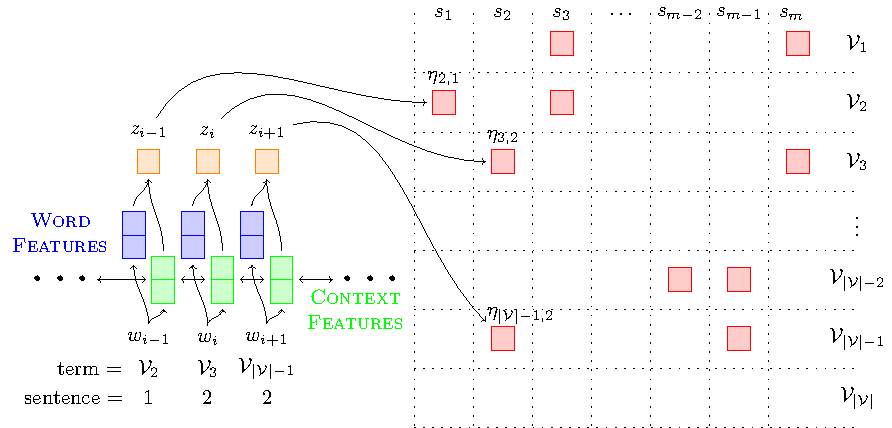
\includegraphics[scale=1.0]{dl_based_salience_models/figures/4_2_wimp_model.pdf}
 \end{center}
 \caption{(Left) Word and context features are extracted from the flat token
sequence representation to get word level importance scores 
$\wordImportance_i$. (Right) Word level scores are aggregated into a sparse
bag-of-words matrix with rows and columns corresponding to sentences and 
words respectively.}
\end{figure}

Our previous experiments revealed that lexical sematics were not the 
main driver of learning in sentence extractive news summarization. 
One could plausibly argue that it is a feature, not a bug, and that 
the structural
signals in news are intentional and not to be avoided. However, we think more 
attention could be paid to estimating importance scores at the word level.
We are motivated by potential application to abstractive generation: better
word level importance estimation could help to remove all but the most 
necessary content from the documents as a preprocessing stage before
abstractive summarization. We are also encouraged by practices
in multi-document news summarization, where word importance weights 
are the main ingredient in sentence representations. 


\newcommand{\classy}{\textsc{Classy}}
\newcommand{\occams}{\textsc{Occams}}

%\subsubsection{A brief discussion of \mlingsys.}

\occams{} and its antecedent \classy{} have been consistent top performers in various
summarization workshops \citep{conroyback,conroyclassy,davis2012occams}. 
In general their main approach 
is to represent each sentence as a sparse bag-of-words, where non-zero
entries correspond to word importance weights for the words found in the 
sentence. Typically, tf-idf weights are used for the importance scores.
The term by sentence matrix representing the document or documents to be
summarized is then factorized into two  matrices (typically with
non-negative entries) representing term factors and sentence factors.
The entries in the sentence factor matrix represent latent ``topics,'' 
and apriori the importance of each sentence is the sum of its latent topic
entries.

Sentence selection can subsequently be performed using one of several methods.
In the naive case, one can select the sentence with the highest vector norm, 
substract the selected latent factors from the remaining sentence vectors
(zeroing out any terms that become negative), and repeating until the
summary length budget is reached. More sophisticated selection procedures
involving multi-dimensional knapsack packing or submodular optimization 
can be used, however these are not the focus of this work.

One draw back to this approach is that the sentence factors and word 
importance scores are unsupervised with respect to the final summarization
objective; their utility to the summarization task is a happy coincidence.
Additionally, the word importance scores are not assigned based on the 
context in which the word appears.

We propose to address these issues by learning word level importance 
scores in the process of single document sentence extractive summarization.
Additionally, we propose a method of adapting these scores from the 
single document case to multi-document summarization.

\subsubsection{Proposed Model}


%In our proposed model for word importance, we first run the \elmo{}model 
%\citep{peters2018deep}
%over the input document to obtain contextual representations
%of each word. The \elmo{}embeddings are then combined with pretrained
%\glove embeddings along with embeddings for document frequency, 
%topic signature,
%sentence position, and part-of-speech tag, and then
%fed into a multi-layer perceptron to predict a scalar importance score.
%When a word occurs multiple times in the input, it can be given a different 
%importance score at each location because the \elmo{} embeddings will capture
%contributions of the salient neighbor words. A term-sentence matrix is 
%then formed from the input, using the estimated word importance scores 
%as the term weights. A sentence extractive summary can be obtained 
%using the naive sentence selection method described above or in 
%\autoref{alg:wimp_ext_alg}.
%The total score for the summary can also be obtained.
%
%We can train this summarizer using a gold extract sequence and a margin loss
%\[\objective(\theta) = \max\big(0, 1 + f(\predSaliences; \theta) - f(\saliences; \theta) \big) \] where $f(\predSaliences;\theta)$ is
%the score of our predicted extract summary.
%
%
%Let $\bowvec_1, \bowvec_2, \dots, \bowvec_n$ be the bag of words 
%representations of the 
%sentences selected for the summary, in the order they were selected.
%The score for the summary is computed as computed by the simple selection
%procedure would be
%$f() = \sum_{i=1}^n \sum_{j=1}^k \max(0, z_{i,j} - \sum_{l=1}^{i-1} z_{l,j})$ 
%
%
%~\\
%~\\

Let $\vocab$ be a finite vocabulary of words. A document $\doc$
is a sequence of $m$ words $(\word_1, \word_2, \ldots, \word_m) \in \vocab^m$.
We define two mappings of words to dense vector representations.
The first $\fdef{\wordFeatures}{\vocab}{\Rn{n_f}}$ maps words to 
a concatenation of feature embeddings whose total dimension is of size $n_f$. 
The various components of the feature embeddings include the word's \glove{} 
embedding, as well as embeddings for sentence position, document frequency,
and other word features that have been shown to be useful for summarization.
The second mapping
$\fdef{\contextFeatures}{\vocab}{\Rn{n_c}}$ maps the word to it's contextual
embedding; here this corresponds to the output of \elmo{} 
\citep{peters2018deep} at that word's
position in the document. 
The importance score $\wordImportance_i$ of a word $\word_i$ is the output of 
a feedforward layer 
\[ \wordImportance_i = \sigma\Big(\mathbf{v}^T \left[\begin{array}{c} \wordFeatures(\word_i) \\ \contextFeatures(\word_i) \end{array} \right] + b \Big) \]
    where $\mathbf{v} \in \Rn{n_f + n_c}$ and $b \in \R$ are learned weight
and bias parameters, and $\sigma$ is the logistic sigmoid.

Next, we aggregate the flat token level scores $\wordImportance_i$ into a
bag-of-words (BOW) 
representation for each sentence in the document.
Let $I_i$ be the set of indices of the flat word sequence corresponding
to the words in $i$-th input sentence. Then, let $\bow_i$ be the BOW 
representation of the $i$-th sentence with entries 
\[ \bow_{i,j} = \begin{cases} 
    0 & \textrm{if $\word_k \ne \vocab_j $ for all $k \in I_i $} \\ 
\sum_{k \in I_i} \mathbbm{1}\{\word_k = \vocab_j \} \cdot \wordImportance_k  & \textrm{otherwise}     \end{cases} \]
        for all $j \in \{1, \ldots, |\vocab|\}$.



\begin{figure}
  \begin{algorithmic}[1]
      \Procedure{\textsc{BowExtracter}}{$\bow_{1:n}, \beta, \kappa$}
   
      \State $\bow_i^{(1)}  \gets \bow_i \quad \forall i \in \{1, \ldots, n\}$
      \State $\hat{\eta} \gets 0$
      \State $t \gets 0$
      \While{ $\sum_{i=1}^t \kappa_{\predLabels_i} < \beta$ and $t < n$}
        \State $t \gets t + 1$
        \State $\predLabels_t \gets \operatorname{arg max}_{i \in \{1,\ldots, n\}}
            \sum_{j=1}^{|\vocab|} \bow^{(t)}_{i,j}$
            \State $\bow_i^{(t+1)} \gets \max(0, \bow_i^{(t)} - \bow^{(t)}_{\predLabels_t} )\quad  \forall i \in \{1, \ldots, n \}$
        \State $\hat{\eta} \gets \hat{\eta} + \sum_{j=1}^{|\vocab|} \bow_{\predLabels_t,j}^{(t)}$
         

      \EndWhile
        \State \Return $[\predLabels_1,\ldots,\predLabels_t], \hat{\eta}$ \Comment{Returns summary sentence indices and summary score.}
    \EndProcedure
  \end{algorithmic}
\caption{Simple sentence extraction algorithm given
 the sentence BOW representations $\omega_i$, 
  a word budget $\beta$, and a vector $\kappa$ of sentence lengths (in words)
  as input.}
\label{alg:wimp_ext_alg}
\end{figure}



        With the BOW representations in hand, we perform sentence selection
        using the algorithm presented in \autoref{alg:wimp_ext_alg} to 
        obtain a predicted extract indices $\predLabels$ and their associated
        overall summary score $\hat{\eta}$.

        We can optimize this model using a margin loss, where given a 
        gold extract sequence  $\labels$, we can compute the associated
        gold extract summary score $\eta$ and then minimize the following
        loss function \[\mathcal{L}_{ext}(\predLabels, \labels;\theta) = \max\big(0, 1 + \hat{\eta} - \eta\big)\]
        with respect to the parameters $\theta$ of the word importance 
        predictor.
        If needed, we can also introduce a supervised learning signal to the 
        individual word importance scores by collecting labels $\zeta_i$ for
        each $\wordImportance_i$ such that $\zeta_i = 1$ if $\word_i$ occurs
        and any human reference abstract and $0$ otherwise. The 
        $\objective_{ext}$ would then be augmented with an additional cross
        entropy loss for the word level predictions:
        \[ \mathcal{L}_{word}(\wordImportance, \zeta; \theta) = -\sum_{i=1}^m \zeta_i \log \wordImportance_i + (1 - \zeta_i) \log (1 - \wordImportance_i). \] 




        \paragraph{Adaptation to MDS} We also propose a simple 
        self attention-based modification to
        the word importance aggregation step to help adapt this method
        to multi-document summarization (MDS). \cite{conroy2013multilingual} 
        found
        that dimensionality reduction on the BOW representations improves
        summarizer performance in the MDS setting (but not as much on
 single document
        summarization). 


        We plan to experiment with the following importance 
        aggregation method. First, given the outputs of the contextual features
        $\mathbf{h}_i = \contextFeatures(\word_i)$, 
        we compute a self attention matrix $\Lambda \in \Rn{m\times m}$
        where \[\Lambda_{i,j} = \sigma(\mathbf{h}_i^T \mathbf{h}_j / \tau + b)  \]
        using sigmoidal attention \citep{kim2017structured} with a learned bias 
        parameter $b$ and a temperature parameter $\tau$.
        Next we compute an attention weighted word importance score $\bar{\wordImportance}_i$ for each word in the input using the following formula,
        \[ \bar{\wordImportance}_i = \sum_{j=1}^m \wordImportance_j \cdot \Lambda_{i,j}.\]
        We then use the aggregated word importance scores 
    $\bar{\wordImportance}_i$ inplace of their nonaggregated counterparts
        in the creating the BOW representations $\omega_j$.

        Our motivation is that by accumulating scores based on context
        similarity, words and topics that appear in multiple documents 
        will accumulate the bulk of the word importance scores, giving 
        an added boost to sentences that contain them. Implicitly, errant
        words from one document that are not on topic to the cluster will
        effectively not contribute much to a sentences score, reducing the 
        effectve dimension of the BOW vectors and regularizing individual
        sentences to the document cluster's mean.

        
        Since we are training our models on single documents, we expect that
        running our pretrainined word scoring model on the individual 
        documents from an MDS document cluster will result in 
        minimal task-adaptation mismatch. The remaining bias and temperature
        parameters can easily be tuned on the small amount of MDS training 
        data available.

%        We also plan to compare this method to using a non-negative matrix 
%        factorization 
%        method on the output of the learned BOW representation, 
%        and to hard attention assignments using Brown clustering.







%\subsubsection{
%\cite{conroy} 


 


\section{Research Plan and Contributions}

\begin{frame}{Research Plan}
    \centering
\begin{tabular}{|ll|}
    \toprule
    \textbf{Task} & \textbf{Date} \\
    \midrule
     Faithful Gen. Impl. & December-February 2019\\
    \hline
    Auto and Human evaluation  & February 2019 - March 2019\\
    \hline
    Word Importance (SDS) &  April 2019 - May 2019 \\
    \hline
    Word Importance (MDS/Genre) & July 2019 \\
    \hline
    Word Importance (Abstractive) & June 2019 \\
    \hline
    Write Thesis & August 2019 - February 2020 \\
    \hline
    !`Defend! & March 2020 \\
    \bottomrule
\end{tabular}


\end{frame}

\begin{frame}{Contributions}
 \begin{itemize}
  \item \textbf{Salience Estimation}
  \begin{itemize}
   \item[\color{green}\ding{51}] Two state-of-the-art sentence extractive 
       stream summarization models. 
       (TREC `14, ACL `15, TREC `15, IJCAI `16)~\\~\\
   \item[\color{green}\ding{51}] State-of-the-art deep learning based sentence
       extractive summarizarization models. 
       (EMNLP `18)~\\~\\
   \item[\color{green}\ding{51}] Extensive ablation studies to determine 
       important lexical/structural features for learning. 
       (EMNLP `18) ~\\~\\
   \item A deep learning model of word importance estimation for 
       single-document news summarization. ~\\~\\
   \item Adaptation of the word importance model to non-news genre and 
       multi-document summarization.
  \end{itemize}
 \end{itemize}
\end{frame}

\begin{frame}{Contributions}
 \begin{itemize}
  \item \textbf{Faithful Generation}
  \begin{itemize}
      \item Supervised attention with word importance estimation.\\~\\
      \item Round-trip Speaker/Listener learning model for:
          \begin{itemize}
              \item data-to-text generation 
              \item text-to-text generation/abstractive summarization.
          \end{itemize}
  \end{itemize}
 \end{itemize}
\end{frame}



%\begin{frame}{Contribution Status}
%
%\begin{itemize}
%
%    \item \textbf{Feature Based Models of Salience} 
%        \begin{itemize}
%            \item[\color{green}\ding{51}] Incorporate salience regression with
%                biased clustering. {\tiny (TREC `14, ACL `15)}
%            \item[\color{green}\ding{51}] Incorporate salience regression with
%                learning to search. {\tiny (TREC `15, IJCAI `16)}
%            \item[\color{green}\ding{51}] Evaluation in {\color{purple}Stream Summarization} task.
%        \end{itemize}
%    \item \textbf{Deep Learning Models of Salience}
%        \begin{itemize}
%            \item[\color{green}\ding{51}] Sentence Level Salience 
%                {\tiny (EMNLP `18)}
%                \begin{itemize}
%                    \item[\color{green}\ding{51}] Implemented simplified DL models.
%                    \item[\color{green}\ding{51}] Model evaluation on 
%                        {\color{purple} Single Document Summarization} task.
%            \item[\color{green}\ding{51}] Extensive ablation studies to determine important 
%                lexical/structural features for learning.
%                \end{itemize}
%            \item[\color{red}\ding{55}] Word level salience.
%                \begin{itemize}
%                    \item[\color{red}\ding{55}] Develop word level DL model and margin learning framework.
%                    \item[\color{red}\ding{55}] Model evaluation on 
%                        {\color{purple}Single Document Summarization} task
%                    \item[\color{red}\ding{55}] Adaption experiments to 
%                        {\color{purple}Multi-Document Summarization} task.
%                    \item[\color{red}\ding{55}] Adaption experiments to 
%                        {\color{purple} Abstractive Summarization} task.
%                \end{itemize}
%        \end{itemize}
%    \item \textbf{Faithful Generation}
%        \begin{itemize}
%            \item[\color{red}\ding{55}] Data-to-Text experiments. (In Progress)
%            \item[\color{red}\ding{55}] Question generation for summarization.
%            \item[\color{red}\ding{55}] Text-to-Text experiments.
%        \end{itemize}
%\end{itemize}
%
%
%
%\end{frame}





%\input{4_data/4_data.tex}
%\input{5_experiments/5_experiments.tex}
%

\begin{frame}{Choice of Sentence \textbf{Encoder}: News}
  \begin{center}
      \begin{tabular}{ccgcg} 
        & & \multicolumn{3}{c}{\textbf{Rouge-2 Recall}}\\
      \toprule
      \textbf{\textsc{Ext}} & \alert{\underline{\textbf{\textsc{Enc}}}}
          & \textbf{CNN/DM} & \textbf{NYT} & \textbf{DUC} \\
      \midrule
      \textsc{Lead}   
         & --         &        $24.4$ &        $32.3$ &   $21.5$  \\
      \hline 
      \multirow{3}{*}{\textsc{Seq2Seq}}
         &\textsc{Avg}&
           \alert{\textbf{25.6}}&\textbf{35.7}&\alert{\textbf{22.8}}  \\
         &\textsc{Rnn}&        25.3 &\textbf{35.9}&        22.5   \\
         &\textsc{Cnn}&        25.1 &        35.1 &\textbf{22.7}  \\
         \hline
      \multirow{3}{*}{\textsc{Cheng \& Lapata}}
         &\textsc{Avg}&
           \alert{25.3}&\textbf{35.6}&\alert{\textbf{23.1}}\\
         &\textsc{Rnn}&        
                     25.0 &          \textbf{35.8} &          \textbf{23.0} \\
         &\textsc{Cnn}&       
                     25.1 &                  35.0  &          \textbf{23.0} \\
         \hline
      \textsc{Oracle} 
         & --         &          36.2 &        48.9 &        31.8   \\
      \bottomrule
    \end{tabular}
    
  \end{center}
  ~\\

  Averaging is either the \alert{\textbf{best}} encoder or 
  \textbf{statistically indistinguishable} from the best encoder!

\end{frame}

\begin{frame}{Choice of Sentence \textbf{Encoder}: Non-News}
  \begin{center}
    \begin{tabular}{ccgcg} 
        & & \multicolumn{3}{c}{\textbf{Rouge-2 Recall}}\\
  \toprule
  \textbf{\textsc{Ext}} & \alert{\underline{\textbf{\textsc{Enc}}}}
      & \textbf{Reddit} & \textbf{AMI} & \textbf{PubMed} \\
  \midrule
  \textsc{Lead}   
     & --         &        $\mathbf{10.9}$ &        $2.0$ &   $9.3$  \\
  \hline
  \multirow{3}{*}{\textsc{Seq2Seq}}
     &\textsc{Avg}&
                   \alert{\textbf{13.6}}&\alert{\textbf{5.5}}&\alert{\textbf{17.7}} \\
     &\textsc{Rnn}&
                   \textbf{12.0}&\textbf{5.3}&        16.7  \\
     &\textsc{Cnn}&
                   \textbf{13.2}&        2.9&        16.9  \\
     \hline
  \multirow{3}{*}{\textsc{Cheng \& Lapata}}
     &\textsc{Avg}&
       \alert{\textbf{13.6}} & \alert{\textbf{6.1}}   & \alert{\textbf{17.7}}\\
     &\textsc{Rnn}&       
       \textbf{12.6} & \textbf{5.0}   & 16.7\\
     &\textsc{Cnn}&       
       \textbf{13.4} & 2.8               &  16.9      \\
     \hline
  \textsc{Oracle} 
     & --         &       16.2    &    3.9     &       25.0   \\
  \bottomrule
\end{tabular}

    
  \end{center}
  ~\\

  Averaging is either the \alert{\textbf{best}} encoder or 
  \textbf{statistically indistinguishable} from the best encoder!
\end{frame}

\begin{frame}{Choice of Sentence \textbf{Extractor}: News}
    
 \begin{center}
   \begin{tabular}{ccgcg}
 & & \multicolumn{3}{c}{\textbf{Rouge-2 Recall}}\\
 \toprule
 \alert{\underline{\textbf{Ext}}} & \textbf{Enc} & 
   \textbf{CNN/DM} & \textbf{NYT} & \textbf{DUC} \\
 \midrule
 \textsc{Lead}    &  --          & 
                   24.4  & 32.3  & 21.5 \\
 \hline
 \textsc{RNN}     & \textsc{Avg} &  
                   25.4  & 34.7  & 22.7 \\
 \hline
 \textsc{Seq2Seq} & \textsc{Avg} & 
           \alert{\textbf{25.6}} & \alert{\textbf{35.7}} & \textbf{22.8} \\
 \hline
 \textsc{Cheng \&  Lapata} & \textsc{Avg} & 
                    25.3 & \textbf{35.6} & \textbf{23.1} \\
 \hline
 \textsc{SummaRunner}  & \textsc{Avg} &  
                    25.4 & 35.4 & 22.3 \\
 \hline
    \textsc{Oracle} & -- & 36.2 &  48.9 &  31.8\\
 \bottomrule
\end{tabular}

 \end{center}
 
 ~\\

 \textsc{Seq2Seq} is the \alert{\textbf{best}} or \textbf{statistically 
 indistinguishable} from the best system.

 ~\\
 \textsc{Rnn} extractor as good as \textsc{SummaRunner} or 
 \textsc{Cheng \& Lapata} extractors on CNN/DailyMail data.

  

\end{frame}

\begin{frame}{Choice of Sentence \textbf{Extractor}: Non-News}
    
 \begin{center}
   \begin{tabular}{ccgcg}
 & & \multicolumn{3}{c}{\textbf{Rouge-2 Recall}}\\
\toprule
\alert{\underline{\textbf{Ext}}} & \textbf{Enc} & 
   \textbf{Reddit} & \textbf{AMI} & \textbf{PubMed} \\
\midrule
\textsc{Lead}    &  --          & 
                   \textbf{10.9}  & 2.0  & 9.3 \\
\hline
\textsc{Rnn}     & \textsc{Avg} &  
                   \textbf{11.4}  & \textbf{5.5}  & 17.0 \\
\hline
\textsc{Seq2Seq} & \textsc{Avg} & 
           \alert{\textbf{13.6}} & \textbf{5.5} & \textbf{17.7} \\
\hline
\textsc{Cheng \&  Lapata} & \textsc{Avg} & 
           \textbf{13.6} & \textbf{6.1} & \textbf{17.7} \\
\hline
\textsc{SummaRunner}  & \textsc{Avg} &  
           \textbf{13.4} & \textbf{5.6} & \textbf{17.2} \\
\hline
    \textsc{Oracle} & -- & 16.2 &  3.9 &  25.0\\
\bottomrule
\end{tabular}


 \end{center}

 ~\\

 \textsc{Seq2Seq} is the \alert{\textbf{best}} or \textbf{statistically indistinguishable} from the best
 system.


\end{frame}



\begin{frame}{Word Embedding Fine-Tuning: (News)}
  \begin{center}
    \begin{tabular}{ccccc}
      & & \multicolumn{3}{c}{\textbf{Rouge-2 Recall}}\\
      \toprule
        \textbf{Ext} & \textbf{Emb}  & 
           \textbf{CNN/DM} & 
           \textbf{NYT} & 
           \textbf{DUC} \\
      \midrule
      \multirow{2}{*}{\textsc{Seq2Seq}} 
        & Fixed & \textbf{25.6} & \textbf{35.7} & \textbf{22.8} \\
        & Fine-Tuned &         25.3  & \textbf{35.7} & \textbf{22.9} \\
      \hline
      \multirow{2}{*}{\textsc{Cheng \& Lapata}} 
        & Fixed & \textbf{25.3} & \textbf{35.6} & \textbf{23.1} \\
        & Fine-Tuned &         24.9  &         35.4  & \textbf{23.0} \\
      \bottomrule
  \end{tabular}


 \end{center}

 ~\\
 
% Performance difference when using \textit{fixed} embeddings versus 
% \textit{fine-tuned} embeddings.
 
  ~\\

%  Models are using the \textsc{Avg} encoder and are initialized with 
%  Glove embeddings. 

%  ~\\

  \textbf{No statistically significant improvement} on news with fine-tuning!

\end{frame}

\begin{frame}{Word Embedding Fine-Tuning: Non-News}
 \begin{center}
  \begin{tabular}{ccccc}
   & & \multicolumn{3}{c}{\textbf{Rouge-2 Recall}}\\
   \toprule
   \textbf{Ext} & \textbf{Emb}  & 
        \textbf{Reddit} & \textbf{AMI} & \textbf{PubMed} \\
   \midrule
   \multirow{2}{*}{\textsc{Seq2Seq}}
      & Fixed & \textbf{13.6} &         5.5  & \textbf{17.7} \\
      & Fine-Tuned & \textbf{13.8} & \textbf{5.8} &         16.9  \\
   \hline
   \multirow{2}{*}{\textsc{Cheng \& Lapata}} 
      & Fixed & \textbf{13.6} & \textbf{6.1} & \textbf{17.7} \\
      & Fine-Tuned & \textbf{13.4} & \textbf{6.2} & \textbf{16.4} \\
   \bottomrule
  \end{tabular}


 \end{center}

 ~\\
 
% Performance difference when using \textit{fixed} embeddings versus 
% \textit{fine-tuned} embeddings.
 
 ~\\

% All models are using the \textsc{Avg} encoder and are initialized with 
% pretrained Glove embeddings from gigaword/wikipedia. 

% ~\\
 \textbf{Statistically significant improvement} with \textsc{Seq2Seq} on AMI
 data. (Caveat: only speech dataset)\\

~\\
Otherwise, same trend as news, \textbf{no stat. sig. improvement} using fine-tuning.

\end{frame}

\begin{frame}{Word Class Ablation: ROUGE-2 Recall}
 \begin{center}
  \begin{tabular}{lcccccc}
   \toprule
   \multirow{1}{*}{\textbf{Ablation}} & 
            \textbf{CNN/DM} & \textbf{NYT} & \textbf{DUC} &
            \textbf{Reddit} & \textbf{AMI} & \textbf{PubMed} \\
   \midrule
     All Words & $\mathbf{25.4}$ & $\mathbf{34.7}$ & $22.7$ &
                  $\mathbf{11.4}$ & $5.5$ & $\mathbf{17.0}$  \\
   \uncover<2->{$-$ Nouns & $25.3$  & $34.3 $ & $22.3$  &
   \alert<2>{$10.3$} & \alert<2>{$3.8$} & \alert<2>{$15.7$}} \\
   \uncover<2->{$-$ Verbs & $25.3$  & $34.4 $ & $22.4$ &
            $10.8$ & $5.8$ & $16.6$ }\\
   \uncover<3->{$-$ Adj/Adv & 
  $25.3$ & $34.4$ & $22.5$ &
   \alert<3>{$9.5$} & $5.4$ & $16.8$} \\
   \uncover<4->{$-$ Function & $25.2$ & $34.6$ & \alert<4>{$\mathbf{22.9}$} &
   $10.3$ & \alert<4>{$\mathbf{6.3}$} & $16.6$ }\\
   \bottomrule
  \end{tabular}
 \end{center}


 %RNN extractor with Averaging encoder. 

 %~\\


 \uncover<2->{\textbf{-Nouns/Verbs} Doesn't decrease performance much on News. Non-News sees small performance drops. }

~\\ 

 \uncover<3->{\textbf{-Adj/Adv} Intensifiers are important in personal stories.
 Signal climactic and important moments.}


 ~\\

 \uncover<4->{\textbf{-Function} Possibly noisy signals on small datasets.}



 ~\\
 \uncover<1-5>{\tiny{\textbf{Bold} is best performance.}}

\end{frame}



\begin{frame}{Shuffled vs In-Order (News)}

 \begin{center}
  \begin{tabular}{ccL{2cm}m{1cm}L{.75cm}} 
   \toprule
   \textbf{Ext.} & \textbf{Order} & 
                           \textbf{CNN/DM} & \textbf{NYT} & \textbf{DUC} \\
   \midrule
%?   \multirow{2}{*}{RNN} 
%?       & In-Order & 
%?       \textbf{25.4} & \textbf{34.7} & \textbf{22.7} \\
%?       & Shuffled & 
%?               22.8 &          25.0  &         18.2  \\
   \multirow{2}{*}{Seq2Seq}
       & In-Order & 
       \textbf{25.6} & \textbf{35.7} &  \textbf{22.8} \\
       & Shuffled & 
               21.7  &         25.6  &          21.2  \\
   \bottomrule
  \end{tabular}
 \end{center}

 ~\\

 Shuffled model is trained on shuffled sentence order documents.

 ~\\

 Both models evaluated on in-order data.


~\\ 
 Large \textbf{performance drops} on news!

\end{frame}

\begin{frame}{Shuffled vs In-Order (Other)}

 \begin{center}
  \begin{tabular}{ccccc} 
   \toprule
   \textbf{Ext.} & \textbf{Order} & 
                           \textbf{Reddit} & \textbf{AMI} & \textbf{PubMed} \\
   \midrule
   \multirow{2}{*}{Seq2Seq}
       & In-Order & 
       \textbf{13.6} &         5.5  &  \textbf{17.7} \\
       & Shuffled & 
       \textbf{13.5} & \textbf{6.0} &          14.9  \\
   \bottomrule
  \end{tabular}
 \end{center}

 ~\\

 Shuffled model is trained on shuffled sentence order documents.

 ~\\

 Both models evaluated on in-order data.

 ~\\

 Small \textbf{performance increase} on AMI.

\end{frame}





\end{document} 
